%%%%%%%%%%%%%%%%%%%%%%%%%%%%%%%%%%%%%%%%%
% The Legrand Orange Book
% LaTeX Template
% Version 2.2 (30/3/17)
%
% This template has been downloaded from:
% http://www.LaTeXTemplates.com
%
% Original author:
% Mathias Legrand (legrand.mathias@gmail.com) with modifications by:
% Vel (vel@latextemplates.com)
%
% License:
% CC BY-NC-SA 3.0 (http://creativecommons.org/licenses/by-nc-sa/3.0/)
%
% Compiling this template:
% This template uses biber for its bibliography and makeindex for its index.
% When you first open the template, compile it from the command line with the 
% commands below to make sure your LaTeX distribution is configured correctly:
%
% 1) pdflatex main
% 2) makeindex main.idx -s StyleInd.ist
% 3) biber main
% 4) pdflatex main x 2
%
% After this, when you wish to update the bibliography/index use the appropriate
% command above and make sure to compile with pdflatex several times 
% afterwards to propagate your changes to the document.
%
% This template also uses a number of packages which may need to be
% updated to the newest versions for the template to compile. It is strongly
% recommended you update your LaTeX distribution if you have any
% compilation errors.
%
% Important note:
% Chapter heading images should have a 2:1 width:height ratio,
% e.g. 920px width and 460px height.
%
%%%%%%%%%%%%%%%%%%%%%%%%%%%%%%%%%%%%%%%%%

%----------------------------------------------------------------------------------------
%	PACKAGES AND OTHER DOCUMENT CONFIGURATIONS
%----------------------------------------------------------------------------------------

\documentclass[11pt,fleqn]{book} % Default font size and left-justified equations

%----------------------------------------------------------------------------------------

%%%%%%%%%%%%%%%%%%%%%%%%%%%%%%%%%%%%%%%%%
% The Legrand Orange Book
% Structural Definitions File
% Version 2.0 (9/2/15)
%
% Original author:
% Mathias Legrand (legrand.mathias@gmail.com) with modifications by:
% Vel (vel@latextemplates.com)
% 
% This file has been downloaded from:
% http://www.LaTeXTemplates.com
%
% License:
% CC BY-NC-SA 3.0 (http://creativecommons.org/licenses/by-nc-sa/3.0/)
%
%%%%%%%%%%%%%%%%%%%%%%%%%%%%%%%%%%%%%%%%%

%----------------------------------------------------------------------------------------
%	VARIOUS REQUIRED PACKAGES AND CONFIGURATIONS
%----------------------------------------------------------------------------------------

\usepackage[top=3cm,bottom=3cm,left=3cm,right=3cm,headsep=10pt,a4paper]{geometry} % Page margins

\usepackage{graphicx} % Required for including pictures
\graphicspath{{Pictures/}} % Specifies the directory where pictures are stored

\usepackage{lipsum} % Inserts dummy text

\usepackage{tikz} % Required for drawing custom shapes

\usepackage[english]{babel} % English language/hyphenation

\usepackage{enumitem} % Customize lists
\setlist{nolistsep} % Reduce spacing between bullet points and numbered lists

\usepackage{booktabs} % Required for nicer horizontal rules in tables

\usepackage{xcolor} % Required for specifying colors by name
\definecolor{ocre}{RGB}{243,102,25} % Define the orange color used for highlighting throughout the book

%----------------------------------------------------------------------------------------
%	FONTS
%----------------------------------------------------------------------------------------

\usepackage{avant} % Use the Avantgarde font for headings
%\usepackage{times} % Use the Times font for headings
\usepackage{mathptmx} % Use the Adobe Times Roman as the default text font together with math symbols from the Sym­bol, Chancery and Com­puter Modern fonts

\usepackage{microtype} % Slightly tweak font spacing for aesthetics
\usepackage[utf8]{inputenc} % Required for including letters with accents
\usepackage[T1]{fontenc} % Use 8-bit encoding that has 256 glyphs

%----------------------------------------------------------------------------------------
%	BIBLIOGRAPHY AND INDEX
%----------------------------------------------------------------------------------------

\usepackage[style=alphabetic,citestyle=numeric,sorting=nyt,sortcites=true,autopunct=true,babel=hyphen,hyperref=true,abbreviate=false,backref=true,backend=bibtex]{biblatex}
\addbibresource{bibliography.bib} % BibTeX bibliography file
\defbibheading{bibempty}{}

\usepackage{calc} % For simpler calculation - used for spacing the index letter headings correctly
\usepackage{makeidx} % Required to make an index
\makeindex % Tells LaTeX to create the files required for indexing

%----------------------------------------------------------------------------------------
%	MAIN TABLE OF CONTENTS
%----------------------------------------------------------------------------------------

\usepackage{titletoc} % Required for manipulating the table of contents

\contentsmargin{0cm} % Removes the default margin

% Part text styling
\titlecontents{part}[0cm]
{\addvspace{20pt}\centering\large\bfseries}
{}
{}
{}

% Chapter text styling
\titlecontents{chapter}[1.25cm] % Indentation
{\addvspace{12pt}\large\sffamily\bfseries} % Spacing and font options for chapters
{\color{ocre!60}\contentslabel[\Large\thecontentslabel]{1.25cm}\color{ocre}} % Chapter number
{\color{ocre}}  
{\color{ocre!60}\normalsize\;\titlerule*[.5pc]{.}\;\thecontentspage} % Page number

% Section text styling
\titlecontents{section}[1.25cm] % Indentation
{\addvspace{3pt}\sffamily\bfseries} % Spacing and font options for sections
{\contentslabel[\thecontentslabel]{1.25cm}} % Section number
{}
{\hfill\color{black}\thecontentspage} % Page number
[]

% Subsection text styling
\titlecontents{subsection}[1.25cm] % Indentation
{\addvspace{1pt}\sffamily\small} % Spacing and font options for subsections
{\contentslabel[\thecontentslabel]{1.25cm}} % Subsection number
{}
{\ \titlerule*[.5pc]{.}\;\thecontentspage} % Page number
[]

% List of figures
\titlecontents{figure}[0em]
{\addvspace{-5pt}\sffamily}
{\thecontentslabel\hspace*{1em}}
{}
{\ \titlerule*[.5pc]{.}\;\thecontentspage}
[]

% List of tables
\titlecontents{table}[0em]
{\addvspace{-5pt}\sffamily}
{\thecontentslabel\hspace*{1em}}
{}
{\ \titlerule*[.5pc]{.}\;\thecontentspage}
[]

%----------------------------------------------------------------------------------------
%	MINI TABLE OF CONTENTS IN PART HEADS
%----------------------------------------------------------------------------------------

% Chapter text styling
\titlecontents{lchapter}[0em] % Indenting
{\addvspace{15pt}\large\sffamily\bfseries} % Spacing and font options for chapters
{\color{ocre}\contentslabel[\Large\thecontentslabel]{1.25cm}\color{ocre}} % Chapter number
{}  
{\color{ocre}\normalsize\sffamily\bfseries\;\titlerule*[.5pc]{.}\;\thecontentspage} % Page number

% Section text styling
\titlecontents{lsection}[0em] % Indenting
{\sffamily\small} % Spacing and font options for sections
{\contentslabel[\thecontentslabel]{1.25cm}} % Section number
{}
{}

% Subsection text styling
\titlecontents{lsubsection}[.5em] % Indentation
{\normalfont\footnotesize\sffamily} % Font settings
{}
{}
{}

%----------------------------------------------------------------------------------------
%	PAGE HEADERS
%----------------------------------------------------------------------------------------

\usepackage{fancyhdr} % Required for header and footer configuration

\pagestyle{fancy}
\renewcommand{\chaptermark}[1]{\markboth{\sffamily\normalsize\bfseries\chaptername\ \thechapter.\ #1}{}} % Chapter text font settings
\renewcommand{\sectionmark}[1]{\markright{\sffamily\normalsize\thesection\hspace{5pt}#1}{}} % Section text font settings
\fancyhf{} \fancyhead[LE,RO]{\sffamily\normalsize\thepage} % Font setting for the page number in the header
\fancyhead[LO]{\rightmark} % Print the nearest section name on the left side of odd pages
\fancyhead[RE]{\leftmark} % Print the current chapter name on the right side of even pages
\renewcommand{\headrulewidth}{0.5pt} % Width of the rule under the header
\addtolength{\headheight}{2.5pt} % Increase the spacing around the header slightly
\renewcommand{\footrulewidth}{0pt} % Removes the rule in the footer
\fancypagestyle{plain}{\fancyhead{}\renewcommand{\headrulewidth}{0pt}} % Style for when a plain pagestyle is specified

% Removes the header from odd empty pages at the end of chapters
\makeatletter
\renewcommand{\cleardoublepage}{
\clearpage\ifodd\c@page\else
\hbox{}
\vspace*{\fill}
\thispagestyle{empty}
\newpage
\fi}

%----------------------------------------------------------------------------------------
%	THEOREM STYLES
%----------------------------------------------------------------------------------------

\usepackage{amsmath,amsfonts,amssymb,amsthm} % For math equations, theorems, symbols, etc

\newcommand{\intoo}[2]{\mathopen{]}#1\,;#2\mathclose{[}}
\newcommand{\ud}{\mathop{\mathrm{{}d}}\mathopen{}}
\newcommand{\intff}[2]{\mathopen{[}#1\,;#2\mathclose{]}}
\newtheorem{notation}{Notation}[chapter]

% Boxed/framed environments
\newtheoremstyle{ocrenumbox}% % Theorem style name
{0pt}% Space above
{0pt}% Space below
{\normalfont}% % Body font
{}% Indent amount
{\small\bf\sffamily\color{ocre}}% % Theorem head font
{\;}% Punctuation after theorem head
{0.25em}% Space after theorem head
{\small\sffamily\color{ocre}\thmname{#1}\nobreakspace\thmnumber{\@ifnotempty{#1}{}\@upn{#2}}% Theorem text (e.g. Theorem 2.1)
\thmnote{\nobreakspace\the\thm@notefont\sffamily\bfseries\color{black}---\nobreakspace#3.}} % Optional theorem note
\renewcommand{\qedsymbol}{$\blacksquare$}% Optional qed square

\newtheoremstyle{blacknumex}% Theorem style name
{5pt}% Space above
{5pt}% Space below
{\normalfont}% Body font
{} % Indent amount
{\small\bf\sffamily}% Theorem head font
{\;}% Punctuation after theorem head
{0.25em}% Space after theorem head
{\small\sffamily{\tiny\ensuremath{\blacksquare}}\nobreakspace\thmname{#1}\nobreakspace\thmnumber{\@ifnotempty{#1}{}\@upn{#2}}% Theorem text (e.g. Theorem 2.1)
\thmnote{\nobreakspace\the\thm@notefont\sffamily\bfseries---\nobreakspace#3.}}% Optional theorem note

\newtheoremstyle{blacknumbox} % Theorem style name
{0pt}% Space above
{0pt}% Space below
{\normalfont}% Body font
{}% Indent amount
{\small\bf\sffamily}% Theorem head font
{\;}% Punctuation after theorem head
{0.25em}% Space after theorem head
{\small\sffamily\thmname{#1}\nobreakspace\thmnumber{\@ifnotempty{#1}{}\@upn{#2}}% Theorem text (e.g. Theorem 2.1)
\thmnote{\nobreakspace\the\thm@notefont\sffamily\bfseries---\nobreakspace#3.}}% Optional theorem note

% Non-boxed/non-framed environments
\newtheoremstyle{ocrenum}% % Theorem style name
{5pt}% Space above
{5pt}% Space below
{\normalfont}% % Body font
{}% Indent amount
{\small\bf\sffamily\color{ocre}}% % Theorem head font
{\;}% Punctuation after theorem head
{0.25em}% Space after theorem head
{\small\sffamily\color{ocre}\thmname{#1}\nobreakspace\thmnumber{\@ifnotempty{#1}{}\@upn{#2}}% Theorem text (e.g. Theorem 2.1)
\thmnote{\nobreakspace\the\thm@notefont\sffamily\bfseries\color{black}---\nobreakspace#3.}} % Optional theorem note
\renewcommand{\qedsymbol}{$\blacksquare$}% Optional qed square
\makeatother

% Defines the theorem text style for each type of theorem to one of the three styles above
\newcounter{dummy} 
\numberwithin{dummy}{section}
\theoremstyle{ocrenumbox}
\newtheorem{theoremeT}[dummy]{Theorem}
\newtheorem{problem}{Problem}[chapter]
\newtheorem{exerciseT}{Exercise}[chapter]
\theoremstyle{blacknumex}
\newtheorem{exampleT}{Example}[chapter]
\theoremstyle{blacknumbox}
\newtheorem{vocabulary}{Vocabulary}[chapter]
\newtheorem{definitionT}{Definition}[section]
\newtheorem{corollaryT}[dummy]{Corollary}
\theoremstyle{ocrenum}
\newtheorem{proposition}[dummy]{Proposition}

%----------------------------------------------------------------------------------------
%	DEFINITION OF COLORED BOXES
%----------------------------------------------------------------------------------------

\RequirePackage[framemethod=default]{mdframed} % Required for creating the theorem, definition, exercise and corollary boxes

% Theorem box
\newmdenv[skipabove=7pt,
skipbelow=7pt,
backgroundcolor=black!5,
linecolor=ocre,
innerleftmargin=5pt,
innerrightmargin=5pt,
innertopmargin=5pt,
leftmargin=0cm,
rightmargin=0cm,
innerbottommargin=5pt]{tBox}

% Exercise box	  
\newmdenv[skipabove=7pt,
skipbelow=7pt,
rightline=false,
leftline=true,
topline=false,
bottomline=false,
backgroundcolor=ocre!10,
linecolor=ocre,
innerleftmargin=5pt,
innerrightmargin=5pt,
innertopmargin=5pt,
innerbottommargin=5pt,
leftmargin=0cm,
rightmargin=0cm,
linewidth=4pt]{eBox}	

% Definition box
\newmdenv[skipabove=7pt,
skipbelow=7pt,
rightline=false,
leftline=true,
topline=false,
bottomline=false,
linecolor=ocre,
innerleftmargin=5pt,
innerrightmargin=5pt,
innertopmargin=0pt,
leftmargin=0cm,
rightmargin=0cm,
linewidth=4pt,
innerbottommargin=0pt]{dBox}	

% Corollary box
\newmdenv[skipabove=7pt,
skipbelow=7pt,
rightline=false,
leftline=true,
topline=false,
bottomline=false,
linecolor=gray,
backgroundcolor=black!5,
innerleftmargin=5pt,
innerrightmargin=5pt,
innertopmargin=5pt,
leftmargin=0cm,
rightmargin=0cm,
linewidth=4pt,
innerbottommargin=5pt]{cBox}

% Creates an environment for each type of theorem and assigns it a theorem text style from the "Theorem Styles" section above and a colored box from above
\newenvironment{theorem}{\begin{tBox}\begin{theoremeT}}{\end{theoremeT}\end{tBox}}
\newenvironment{exercise}{\begin{eBox}\begin{exerciseT}}{\hfill{\color{ocre}\tiny\ensuremath{\blacksquare}}\end{exerciseT}\end{eBox}}				  
\newenvironment{definition}{\begin{dBox}\begin{definitionT}}{\end{definitionT}\end{dBox}}	
\newenvironment{example}{\begin{exampleT}}{\hfill{\tiny\ensuremath{\blacksquare}}\end{exampleT}}		
\newenvironment{corollary}{\begin{cBox}\begin{corollaryT}}{\end{corollaryT}\end{cBox}}	

%----------------------------------------------------------------------------------------
%	REMARK ENVIRONMENT
%----------------------------------------------------------------------------------------

\newenvironment{remark}{\par\vspace{10pt}\small % Vertical white space above the remark and smaller font size
\begin{list}{}{
\leftmargin=35pt % Indentation on the left
\rightmargin=25pt}\item\ignorespaces % Indentation on the right
\makebox[-2.5pt]{\begin{tikzpicture}[overlay]
\node[draw=ocre!60,line width=1pt,circle,fill=ocre!25,font=\sffamily\bfseries,inner sep=2pt,outer sep=0pt] at (-15pt,0pt){\textcolor{ocre}{R}};\end{tikzpicture}} % Orange R in a circle
\advance\baselineskip -1pt}{\end{list}\vskip5pt} % Tighter line spacing and white space after remark

%----------------------------------------------------------------------------------------
%	SECTION NUMBERING IN THE MARGIN
%----------------------------------------------------------------------------------------

\makeatletter
\renewcommand{\@seccntformat}[1]{\llap{\textcolor{ocre}{\csname the#1\endcsname}\hspace{1em}}}                    
\renewcommand{\section}{\@startsection{section}{1}{\z@}
{-4ex \@plus -1ex \@minus -.4ex}
{1ex \@plus.2ex }
{\normalfont\large\sffamily\bfseries}}
\renewcommand{\subsection}{\@startsection {subsection}{2}{\z@}
{-3ex \@plus -0.1ex \@minus -.4ex}
{0.5ex \@plus.2ex }
{\normalfont\sffamily\bfseries}}
\renewcommand{\subsubsection}{\@startsection {subsubsection}{3}{\z@}
{-2ex \@plus -0.1ex \@minus -.2ex}
{.2ex \@plus.2ex }
{\normalfont\small\sffamily\bfseries}}                        
\renewcommand\paragraph{\@startsection{paragraph}{4}{\z@}
{-2ex \@plus-.2ex \@minus .2ex}
{.1ex}
{\normalfont\small\sffamily\bfseries}}

%----------------------------------------------------------------------------------------
%	PART HEADINGS
%----------------------------------------------------------------------------------------

% numbered part in the table of contents
\newcommand{\@mypartnumtocformat}[2]{%
\setlength\fboxsep{0pt}%
\noindent\colorbox{ocre!20}{\strut\parbox[c][.7cm]{\ecart}{\color{ocre!70}\Large\sffamily\bfseries\centering#1}}\hskip\esp\colorbox{ocre!40}{\strut\parbox[c][.7cm]{\linewidth-\ecart-\esp}{\Large\sffamily\centering#2}}}%
%%%%%%%%%%%%%%%%%%%%%%%%%%%%%%%%%%
% unnumbered part in the table of contents
\newcommand{\@myparttocformat}[1]{%
\setlength\fboxsep{0pt}%
\noindent\colorbox{ocre!40}{\strut\parbox[c][.7cm]{\linewidth}{\Large\sffamily\centering#1}}}%
%%%%%%%%%%%%%%%%%%%%%%%%%%%%%%%%%%
\newlength\esp
\setlength\esp{4pt}
\newlength\ecart
\setlength\ecart{1.2cm-\esp}
\newcommand{\thepartimage}{}%
\newcommand{\partimage}[1]{\renewcommand{\thepartimage}{#1}}%
\def\@part[#1]#2{%
\ifnum \c@secnumdepth >-2\relax%
\refstepcounter{part}%
\addcontentsline{toc}{part}{\texorpdfstring{\protect\@mypartnumtocformat{\thepart}{#1}}{\partname~\thepart\ ---\ #1}}
\else%
\addcontentsline{toc}{part}{\texorpdfstring{\protect\@myparttocformat{#1}}{#1}}%
\fi%
\startcontents%
\markboth{}{}%
{\thispagestyle{empty}%
\begin{tikzpicture}[remember picture,overlay]%
\node at (current page.north west){\begin{tikzpicture}[remember picture,overlay]%	
\fill[ocre!20](0cm,0cm) rectangle (\paperwidth,-\paperheight);
\node[anchor=north] at (4cm,-3.25cm){\color{ocre!40}\fontsize{220}{100}\sffamily\bfseries\thepart}; 
\node[anchor=south east] at (\paperwidth-1cm,-\paperheight+1cm){\parbox[t][][t]{8.5cm}{
\printcontents{l}{0}{\setcounter{tocdepth}{1}}%
}};
\node[anchor=north east] at (\paperwidth-1.5cm,-3.25cm){\parbox[t][][t]{15cm}{\strut\raggedleft\color{white}\fontsize{30}{30}\sffamily\bfseries#2}};
\end{tikzpicture}};
\end{tikzpicture}}%
\@endpart}
\def\@spart#1{%
\startcontents%
\phantomsection
{\thispagestyle{empty}%
\begin{tikzpicture}[remember picture,overlay]%
\node at (current page.north west){\begin{tikzpicture}[remember picture,overlay]%	
\fill[ocre!20](0cm,0cm) rectangle (\paperwidth,-\paperheight);
\node[anchor=north east] at (\paperwidth-1.5cm,-3.25cm){\parbox[t][][t]{15cm}{\strut\raggedleft\color{white}\fontsize{30}{30}\sffamily\bfseries#1}};
\end{tikzpicture}};
\end{tikzpicture}}
\addcontentsline{toc}{part}{\texorpdfstring{%
\setlength\fboxsep{0pt}%
\noindent\protect\colorbox{ocre!40}{\strut\protect\parbox[c][.7cm]{\linewidth}{\Large\sffamily\protect\centering #1\quad\mbox{}}}}{#1}}%
\@endpart}
\def\@endpart{\vfil\newpage
\if@twoside
\if@openright
\null
\thispagestyle{empty}%
\newpage
\fi
\fi
\if@tempswa
\twocolumn
\fi}

%----------------------------------------------------------------------------------------
%	CHAPTER HEADINGS
%----------------------------------------------------------------------------------------

% A switch to conditionally include a picture, implemented by  Christian Hupfer
\newif\ifusechapterimage
\usechapterimagetrue
\newcommand{\thechapterimage}{}%
\newcommand{\chapterimage}[1]{\ifusechapterimage\renewcommand{\thechapterimage}{#1}\fi}%
\newcommand{\autodot}{.}
\def\@makechapterhead#1{%
{\parindent \z@ \raggedright \normalfont
\ifnum \c@secnumdepth >\m@ne
\if@mainmatter
\begin{tikzpicture}[remember picture,overlay]
\node at (current page.north west)
{\begin{tikzpicture}[remember picture,overlay]
\node[anchor=north west,inner sep=0pt] at (0,0) {\ifusechapterimage\includegraphics[width=\paperwidth]{\thechapterimage}\fi};
\draw[anchor=west] (\Gm@lmargin,-9cm) node [line width=2pt,rounded corners=15pt,draw=ocre,fill=white,fill opacity=0.5,inner sep=15pt]{\strut\makebox[22cm]{}};
\draw[anchor=west] (\Gm@lmargin+.3cm,-9cm) node {\huge\sffamily\bfseries\color{black}\thechapter\autodot~#1\strut};
\end{tikzpicture}};
\end{tikzpicture}
\else
\begin{tikzpicture}[remember picture,overlay]
\node at (current page.north west)
{\begin{tikzpicture}[remember picture,overlay]
\node[anchor=north west,inner sep=0pt] at (0,0) {\ifusechapterimage\includegraphics[width=\paperwidth]{\thechapterimage}\fi};
\draw[anchor=west] (\Gm@lmargin,-9cm) node [line width=2pt,rounded corners=15pt,draw=ocre,fill=white,fill opacity=0.5,inner sep=15pt]{\strut\makebox[22cm]{}};
\draw[anchor=west] (\Gm@lmargin+.3cm,-9cm) node {\huge\sffamily\bfseries\color{black}#1\strut};
\end{tikzpicture}};
\end{tikzpicture}
\fi\fi\par\vspace*{270\p@}}}

%-------------------------------------------

\def\@makeschapterhead#1{%
\begin{tikzpicture}[remember picture,overlay]
\node at (current page.north west)
{\begin{tikzpicture}[remember picture,overlay]
\node[anchor=north west,inner sep=0pt] at (0,0) {\ifusechapterimage\includegraphics[width=\paperwidth]{\thechapterimage}\fi};
\draw[anchor=west] (\Gm@lmargin,-9cm) node [line width=2pt,rounded corners=15pt,draw=ocre,fill=white,fill opacity=0.5,inner sep=15pt]{\strut\makebox[22cm]{}};
\draw[anchor=west] (\Gm@lmargin+.3cm,-9cm) node {\huge\sffamily\bfseries\color{black}#1\strut};
\end{tikzpicture}};
\end{tikzpicture}
\par\vspace*{270\p@}}
\makeatother

%----------------------------------------------------------------------------------------
%	HYPERLINKS IN THE DOCUMENTS
%----------------------------------------------------------------------------------------

\usepackage{hyperref}
\hypersetup{hidelinks,backref=true,pagebackref=true,hyperindex=true,colorlinks=false,breaklinks=true,urlcolor= ocre,bookmarks=true,bookmarksopen=false,pdftitle={Title},pdfauthor={Author}}
\usepackage{bookmark}
\bookmarksetup{
open,
numbered,
addtohook={%
\ifnum\bookmarkget{level}=0 % chapter
\bookmarksetup{bold}%
\fi
\ifnum\bookmarkget{level}=-1 % part
\bookmarksetup{color=ocre,bold}%
\fi
}
}
 % Insert the commands.tex file which contains the majority of the structure behind the template

\begin{document}

%----------------------------------------------------------------------------------------
%	TITLE PAGE
%----------------------------------------------------------------------------------------

\begingroup
\thispagestyle{empty}
\begin{tikzpicture}[remember picture,overlay]
\node[inner sep=0pt] (background) at (current page.center) {
\includegraphics[width=\paperwidth]{background}};
\draw (current page.center) node [fill=ocre!30!white,fill opacity=0.6,text opacity=1,inner sep=1cm]{\Huge\centering\bfseries\sffamily\parbox[c][][t]{\paperwidth}{\centering The Search for a Title\\[15pt] % Book title
{\Large A Profound Subtitle}\\[20pt] % Subtitle
{\huge Dr. John Smith}}}; % Author name
\end{tikzpicture}
\vfill
\endgroup

%----------------------------------------------------------------------------------------
%	COPYRIGHT PAGE
%----------------------------------------------------------------------------------------

\newpage
~\vfill
\thispagestyle{empty}

\noindent Copyright \copyright\ 2013 John Smith\\ % Copyright notice

\noindent \textsc{Published by Publisher}\\ % Publisher

\noindent \textsc{book-website.com}\\ % URL

\noindent Licensed under the Creative Commons Attribution-NonCommercial 3.0 Unported License (the ``License''). You may not use this file except in compliance with the License. You may obtain a copy of the License at \url{http://creativecommons.org/licenses/by-nc/3.0}. Unless required by applicable law or agreed to in writing, software distributed under the License is distributed on an \textsc{``as is'' basis, without warranties or conditions of any kind}, either express or implied. See the License for the specific language governing permissions and limitations under the License.\\ % License information

\noindent \textit{First printing, March 2013} % Printing/edition date

%----------------------------------------------------------------------------------------
%	TABLE OF CONTENTS
%----------------------------------------------------------------------------------------

%\usechapterimagefalse % If you don't want to include a chapter image, use this to toggle images off - it can be enabled later with \usechapterimagetrue

\chapterimage{chapter_head_1.pdf} % Table of contents heading image

\pagestyle{empty} % No headers

\tableofcontents % Print the table of contents itself

\cleardoublepage % Forces the first chapter to start on an odd page so it's on the right

\pagestyle{fancy} % Print headers again

%----------------------------------------------------------------------------------------
%	PART
%----------------------------------------------------------------------------------------

\part{Part One}

%----------------------------------------------------------------------------------------
%	CHAPTER 1
%----------------------------------------------------------------------------------------

\chapterimage{chapter_head_2.pdf} % Chapter heading image

\chapter{Geometri Bidang Datar}
\section{Kesebangunan antar bangun datar}\index{Paragraphs of Text}


Kesebangunan dan kekongruenan biasanya digunakan untuk membandingkan dua buah bangun datar (atau lebih) dengan bentuk yang sama. dua buah bangun datar dapat dikatakan sebangun apabila panjang setiap sisi pada kedua bangun datar tersebut memiliki nilai perbandingan yang sama. sedangkan kongruen memiliki konsep yang lebih mendetail, apabila dua buah (atau lebih) bangun datar memiliki bentuk, ukuran, serta besar sudut yang sama barulah mereka dapat disebut sebagai bangun datar yang kongruen.Perhatikan gambar berikut:

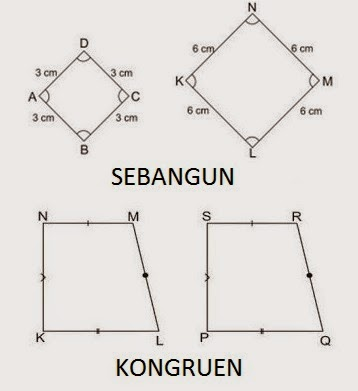
\includegraphics[width=3cm,height=3cm]{Kesebangunan.jpg}


Kesebangunan Pada Persegi Panjang

Perhatikan gambar dua buah persegi panjang di bawah ini.keduanya merupakan bangun datar yang sebangun karena memiliki kesamaan sifat yang dapat dijelaskan sebagai berikut:

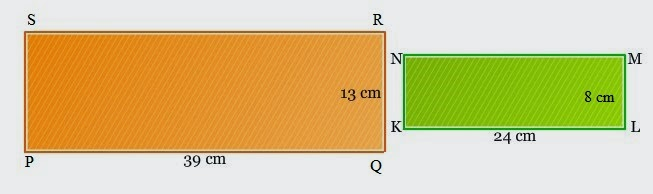
\includegraphics[width=3cm,height=3cm]{persegi.jpg}


\textbf{1.Perbandingan antara sisi terpanjang dengan sisi terpendek memiliki nilai yang sama.}

Perbandingan sisi terpanjang PQ dengan sisi terpendek QR  = 39 : 13  = 1 : 3
Perbandingan sisi terpanjang KL dengan sisi terpendek LM   = 24 : 8    = 1 : 3
Perbandingan sisi terpanjang RS dengan sisi terpendek QP   = 39 : 13  = 1 : 3
Perbandingan sisi terpanjang MN dengan sisi terpendek NK = 24 : 8    = 1 : 3

Dari perhitungan diatas dapat dilihat bahwa sisi terpanjang dan terpendek pada kedua persegi panjang diatas  memiliki perbandingan yang sama yaitu 1 : 3.


\textbf{2.Besar sudut pada kedua persegi panjang tersebut memiliki nilai yang sama besar.}

Sudut P = Sudut K; Sudut Q = Sudut L; Sudut R = Sudut M; Sudut S = Sudut N

Karena kedua persegi panjang tersebut hanya memiliki bentuk dan sudut yang sama besar namun tidak memiliki ukuran yang sama, maka dua bangun datar tersebut tidak bisa disebut kongruen.

\textbf{Contoh Soal Kesebangunan pada Persegi Panjang}

Ada dua buah persegi panjang dengan ukuran yang berbeda ABCD dan KLMN. Persegi panjang ABCD memiliki panjang 16cm dan lebar 4cm. Bila persegi panjang ABCD sebangun dengan persegi panjang KLMN yang memiliki panjang 32cm, maka berapakah lebar dari persegi panjang KLMN?

Karena kedua persegi panjang tersebut sebangun, maka berlaku rumus:

AB/KL = BC/LM
16/32 = 4/LM
   LM = 32x4/16
   LM = 124/16
   LM = 8 cm

Maka lebar dari persegi panjang KLMN adalah 8 cm.


Kesebangunan pada Segitiga
Kesebangunan pada segitiga agak lebih sulit dicapai karena ada tiga buah sisi yang harus sama perbandingannya. 

Contoh segitiga yang sebangun:


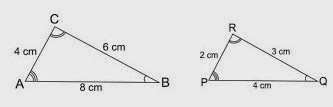
\includegraphics[width=3cm,height=3cm]{segitiga.jpg}


Segitiga tersebut dapat dikatakan sebangun karena perbandingan sisi-sisinya sama besar:

Sisi AC sesuai dengan sisi PR = AC/PR = 4/2 = 2/1
Sisi AB sesuai dengan sisi PQ = AB/PQ = 8/4 = 2/1
Sisi BC sesuai dengan sisi QR = BC/QR = 6/3 = 2/1

Maka AC/PR = AB/PQ = BC/QR = 2/1


Besar sudut yang bersesuaian memiliki besar yang sama:

Sudut A = sudut P; sudut B = sudut Q; sudut C = sudut R

\textbf{Contoh Soal Kesebangunan pada Persegi Panjang}


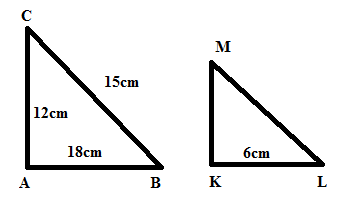
\includegraphics[width=3cm,height=3cm]{soal.jpg}


Diketahui segitiga ABC sebangun dengan segitiga KLM, maka berapakah panjang LM dan MK?

Jawab:

AB/KL = BC/LM
18/6  = 15/LM
   3  = 15/LM
   LM = 15/3
   LM = 5 cm

Dari hasil tersebut kita dapat mengetahui bahwa perbandingan sisi pada kedua segitiga tersebut adalah:

18 : 6 = 3 : 1
15 : 5 = 3 : 1
12 : MK = 3 : 1
MK = 12/3
MK = 4 cm
\\

\textbf{Contoh Kesebangunan pada Trapesium}

Perhatikan gambar di bawah ini!

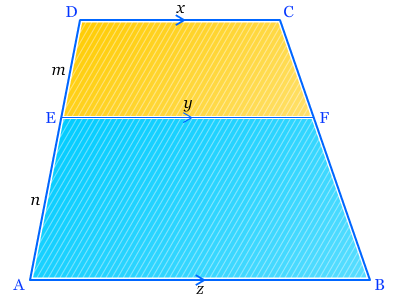
\includegraphics[width=3cm,height=3cm]{soal1.jpg}

Buktikan bahwa,

Soal 6 Rumus

Jika DC = 20 cm, AB = 34 cm, DE = 9 cm dan AE = 15 cm, tentukan EF!

Pembahasan Untuk membuktikan rumus yang ditentukan, kita harus menggambar garis DH yang sejajar dengan garis BC, seperti berikut.
Karena garis EG sejajar dengan garis AH, maka segitiga DEG sebangun dengan segitiga DAH. Akibatnya,

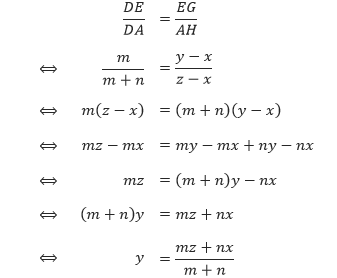
\includegraphics[width=3cm,height=3cm]{rumus1.jpg}

Untuk DC = 20 cm, AB = 34 cm, DE = 9 cm dan AE = 15 cm, maka

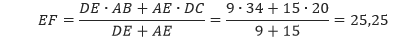
\includegraphics[width=3cm,height=3cm]{rumus2.jpg}
Jadi, diperoleh panjang EF adalah 25,25 cm..

1.Diberikan dua buah persegipanjang ABCD dan persegipanjang PQRS seperti gambar berikut.

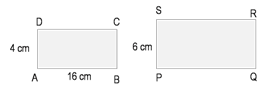
\includegraphics[width=5cm,height=5cm]{1adli.png}
Kedua persegipanjang tersebut adalah sebangun. Tentukan:
a) panjang PQ
b) luas dan keliling persegipanjang PQRS

Pembahasan
a) Perbandingan panjang garis AB dengan AD bersesuaian dengan perbandingan panjang garis PQ dengan PS. Sehingga
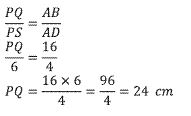
\includegraphics[width=5cm,height=5cm]{1adli.jpg}
Panjang PQ = 24 cm
b) Luas persegipanjang PQRS = PQ x PS = 24 cm x 6 cm = 144 cm2
Keliling persegipanjang PQRS = 2 x (PQ + PS) = 2 x (24 cm + 6 cm) = 60 cm

2.Perhatikan gambar berikut! 
 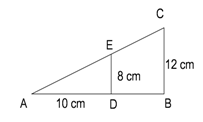
\includegraphics[width=5cm,height=5cm]{2adli.png}
Tentukan panjang DB!

Pembahasan
Soal ini tentang kesebangunan segitiga. Segitiga ABC yang lebih besar sebangun dengan segitiga kecil ADE sehingga perbandingan panjang sisi-sisi yang bersesuaian akan sama. Temukan dulu panjang sisi AB, ambil perbandingan alas dan tinggi dari kedua segitiga seperti berikut ini:
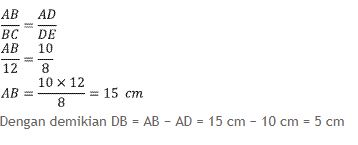
\includegraphics[width=6cm,height=6cm]{2adli.jpg}

3.Dari soal berikut, tentukan:
 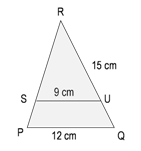
\includegraphics[width=5cm,height=5cm]{3adli.png}
 
a) QR
b) QU

Pembahasan
a) Penyelesaian seperti nomor 2, ambil perbandingan sisi-sisi yang bersesuaian dari segitiga PQR dan segitiga SUR. 

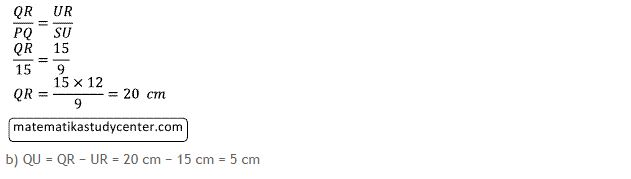
\includegraphics[width=6cm,height=6cm]{3adli.jpg}

4.Perhatikan gambar berikut! 
 
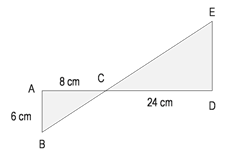
\includegraphics[width=5cm,height=5cm]{4adli.png}
Tentukan panjang DE

Pembahasan
Kesebangunan dua segitiga siku-siku 
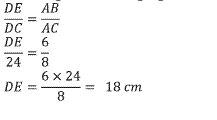
\includegraphics[width=5cm,height=5cm]{4adli.jpg}

5.Dari soal berikut tentukan panjang DE! 
 
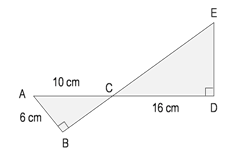
\includegraphics[width=5cm,height=5cm]{5adli.png}

Pembahasan
Bedakan pengambilan sisi-sisi yang bersesuaian dari soal nomor sebelumnya. 
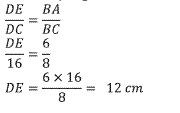
\includegraphics[width=5cm,height=5cm]{5adli.jpg}

6.Diketahui panjang SR adalah 8 cm. 

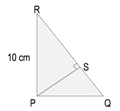
\includegraphics[width=5cm,height=5cm]{6adli.png}
Tentukan panjang QS!

Pembahasan
Kongruensi dua segitiga siku-siku, tentukan lebih dahulu panjang PS gunakan teorema phytagoras akan didapat angka 6 cm untuk panjang PS. Kemudian lakukan perbandingan sisi yang sesuai: 
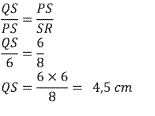
\includegraphics[width=5cm,height=5cm]{6adli.jpg}

7.Dari soal berikut ini tentukan panjang EF! 
 
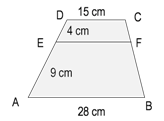
\includegraphics[width=5cm,height=5cm]{7adli.png}
Pembahasan
Buat satu garis yang sejajar dengan garis AD namakan CH seperti gambar berikut. 

\includegraphics[width=5cm,height=5cm]{7adli1.png}
Terlihat muncul  data-data baru yaitu EG = 15 cm, AH = 15 cm dan HB = 13 cm. Ambil dua segitiga sebangun GFC dan HBC bandingkan sisi-sisi yang bersesuaian:

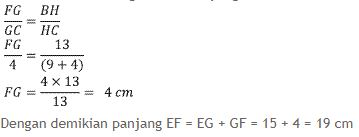
\includegraphics[width=5cm,height=5cm]{7adli.jpg}

8.Perhatikan gambar berikut ini. 

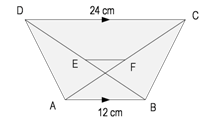
\includegraphics[width=5cm,height=5cm]{8adli.png}

Tentukan panjang EF, jika titik E dan titik F berturut-turut adalah titik tengah diagonal DB dan diagonal CA!

Pembahasan
Cara pertama,
Perhatikan garis DB yang dibagi menjadi segmen-segmen DE, EG dan GB. 
Misalkan 
panjang DB adalah 2a 
maka 
DE = a 
EB = a 

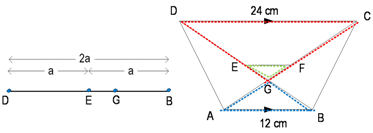
\includegraphics[width=5cm,height=5cm]{8adli1.png}

Dari kesebangunan segitiga DGC dan segitiga AGB didapatkan perbandingan panjang garis
DG : GB = 2 : 1  didapatnya  dari 24 cm : 12 cm

Sehingga

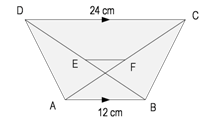
\includegraphics[width=5cm,height=5cm]{8adli.jpg}

Dari pembagian segmen garis DB terlihat bahwa
DG = DE + GE
Sehingga

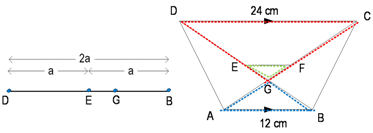
\includegraphics[width=5cm,height=5cm]{8adli1.jpg}

Akhirnya bandingkan sisi-sisi yang bersesuaian pada segitiga kongruen ABG dan EGF. 

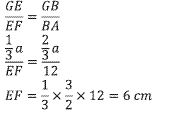
\includegraphics[width=5cm,height=5cm]{8adli2.jpg}

Cara kedua,  namun diingat hanya untuk tipe soal seperti ini saja, jadi titik E dan F nya di tengah-tengah, jangan gunakan untuk tipe soal yang lain: 

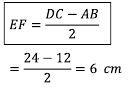
\includegraphics[width=5cm,height=5cm]{8adli3.jpg}

9.Perhatikan gambar berikut ini! 

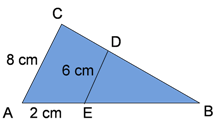
\includegraphics[width=5cm,height=5cm]{9adli.png}

Jarak titik E ke B adalah....
A. 1,5
B. 6
C. 8
D. 10 

Pembahasan
Misalkan EB dinamakan x, maka AB nantinya akan sama dengan (2 + x). Perbandingan sisi EB dengan ED pada segitiga kecil (segitiga BDE), harus sama dengan perbandingan AB dengan AC pada segitiga besar (segitiga BCA). Selanjutnya: 

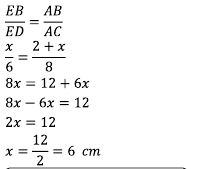
\includegraphics[width=5cm,height=5cm]{9adli.jpg}
 
Jadi panjang EB adalah 6 cm.

10.Perhatikan gambar berikut ini! 

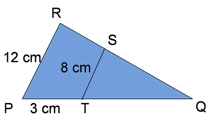
\includegraphics[width=5cm,height=5cm]{10adli.png}

Panjang TQ adalah...
A. 4
B. 5
C. 6
D. 7

(UN 2007) 

Pembahasan
Dengan cara yang sama dengan nomor 9 diperoleh: 

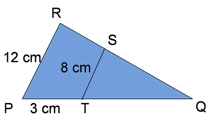
\includegraphics[width=5cm,height=5cm]{10adli.jpg}

11. Sebuah karton berukuran tinggi 30 cm dan lebar 20 cm. Budi menempelkan sebuah foto sehingga sisa karton di sebelah kiri, kanan, atas foto adalah 2 cm.

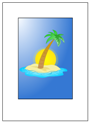
\includegraphics[width=5cm,height=5cm]{11adli.png}

Jika foto dan karton sebangun, sisa karton di bawah foto adalah...
A. 5 cm 
B. 4 cm 
C. 3 cm 
D. 2 cm 

(Modifikasi Soal Kesebangunan - UN 2010)

Pembahasan
Perhatikan ilustrasi foto dan karton tempat menempel berikut, misalkan sisa panjang karton namakan sebagai x.

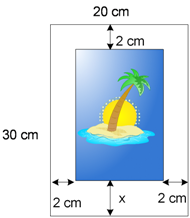
\includegraphics[width=5cm,height=5cm]{11adli1.png}

Perbandingan panjang dengan lebar foto harus sama dengan perbandingan panjang dengan lebar dari karton, karena sebangun. 

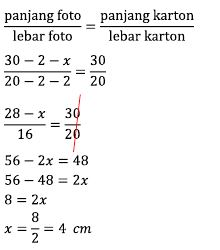
\includegraphics[width=5cm,height=5cm]{11adli.jpg}

12.Sebuah foto berukuran tinggi 30 cm dan lebar 20 cm ditempel pada sebuah karton. Sisa karton di sebelah kiri, kanan, atas foto 2 cm. Jika foto dan karton sebangun, sisa karton di bawah foto adalah...
A. 5 cm 
B. 4 cm 
C. 3 cm 
D. 2 cm 
(Soal Kesebangunan - Soal UN Matematika 2010) 

Pembahasan
Perhatikan ilustrasi foto dan karton tempat menempel berikut, 

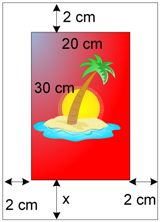
\includegraphics[width=5cm,height=5cm]{12adli.png}

Perbandingan panjang dengan lebar foto harus sama dengan perbandingan panjang dengan lebar dari karton, karena sebangun.
Perhatikan perbedaannya dengan nomor sebelumnya dalam menempatkan x.

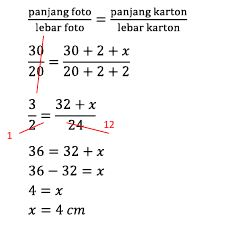
\includegraphics[width=5cm,height=5cm]{12adli.jpg}

13.Perhatikan gambar! 

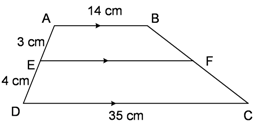
\includegraphics[width=5cm,height=5cm]{13adli.png}

Panjang EF adalah...
A. 20 cm
B. 21 cm
C. 23 cm
D. 26 cm

(UN SMP 2013)

Pembahasan
Tambahaan garis bantu, beri nama BG. 

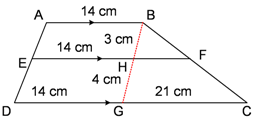
\includegraphics[width=5cm,height=5cm]{13adli1.png}

Panjang DG jadi 14 cm, dan GC 21 cm karena tadinya DC = 35 cm. Bandingkan sisi segitiga besar BGC dan segitiga kecil BHF yang bersesuaian hingga diperoleh panjang HF dulu. 

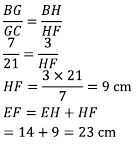
\includegraphics[width=5cm,height=5cm]{13adli.jpg}

Soal No. 14
Perhatikan gambar di samping! 

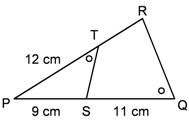
\includegraphics[width=5cm,height=5cm]{14adli.png}

Panjang TR adalah….
A. 2 cm
B. 3 cm
C. 4 cm
D. 6 cm

(UN Matematika SMP/MTs tahun 2014)

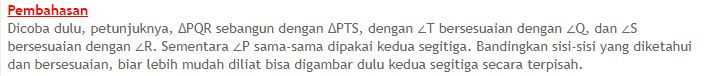
\includegraphics[width=15cm,height=8cm]{14adli.jpg}

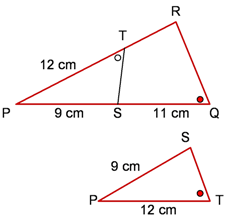
\includegraphics[width=5cm,height=5cm]{14adli1.png}


\section{Kekongruenan Antar Bangun Datar}\index{Paragraphs of Text}

Definisi kekongruenan tidak lepas dari kesebangunan karena kekongruenan
merupakan kasus khusus kesebangunan. Jadi definisinya sebagai berikut.
Dua segibanyak (polygon) dikatakan kongruen jika ada korespondensi satu-satu
antara titik-titik sudut kedua segi banyak tersebut sedemikian hingga berlaku: 

1. sudut-sudut yang bersesuaian sama besar, dan

2. semua perbandingan panjang sisi-sisi yang bersesuaian adalah satu.

Syarat kedua ini dapat diringkas menjadi 2`. sisi-sisi yang bersesuaian sama panjang. 

%------------------------------------------------

\subsection{Pengertian Kesebangunan}

Perhatikan gambar persegi panjang ABCD dan PQRS di bawah ini! Pada persegi panjang ABCD memiliki panjang dan lebar yaitu 36 mm dan 24 mm, serta persegi panjang PQRS memiliki panjang dan lebar yaitu 58 mm dan 38 mm.

 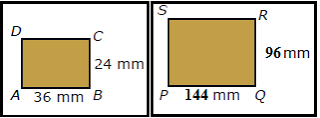
\includegraphics[width=8cm,height=5cm]{h1_1.png}\\
 
Perbandingan antara panjang persegipanjang ABCD dan panjang persegi panjang PQRS adalah 36 : 144 atau 1 : 4. Demikian pula dengan lebarnya, perbandingannya 24 : 96 atau 1 : 4. Dengan demikian, sisi-sisi yang bersesuaian dari kedua persegipanjang itu memiliki perbandingan senilai (sebanding). Perbandingan sisi yang bersesuaian dari kedua persegipanjang tersebut, yaitu sebagai berikut.\\
AB/PQ = BC/QR = CD/RS = AD/PS = 1/4\\

Oleh karena semua sudut persegipanjang besarnya 90 derajat (siku-siku) maka sudut-sudut yang bersesuaian dari kedua persegipanjang itu besarnya sama. Dalam hal ini, persegipanjang ABCD dan persegipanjang PQRS memiliki sisi-sisi bersesuaian yang sebanding dan sudut-sudut bersesuaian yang sama besar. Selanjutnya, kedua persegipanjang tersebut dikatakan sebangun. Jadi, persegipanjang ABCD sebangun dengan persegipanjang PQRS.\\

Pengertian kesebangunan seperti ini berlaku umum untuk setiap bangun datar. Dua bangun datar dikatakan sebangun jika memenuhi dua syarat berikut.\\

Panjang sisi-sisi yang bersesuaian dari kedua bangun itu memiliki perbandingan senilai.
Sudut-sudut yang bersesuaian dari kedua bangun itu sama besar.\\


Contoh Soal 1\\
Jika persegipanjang ABCD sebangun dengan persegi panjang PQRS, hitung panjang QR.\\
 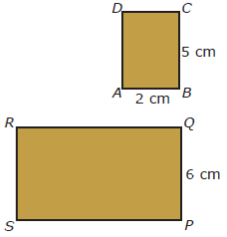
\includegraphics[width=6cm,height=6cm]{h1_2.png}\\
 
Penyelesaian:
Salah satu syarat dua bangun dikatakan sebangun adalah sisi-sisi yang bersesuaian sebanding. Oleh karena itu,\\
AB/PQ = BC/QR\\
2/6 = 5/QR\\
2QR = 30\\
QR = 15\\
Jadi, panjang QR adalah 15 cm.\\


Contoh Soal 2\\
Jika layang-layang KLMN dan layang-layang PQRS pada gambar di bawah ini sebangun, tentukan besar sudut R dan sudut S.\\
 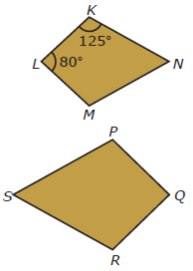
\includegraphics[width=6cm,height=6cm]{h1_3.png}\\

Penyelesaian:
Salah satu syarat dua bangun dikatakan sebangun adalah sudut-sudut yang bersesuaian sama besar sehingga sudut P = 125derajat dan sudut Q = 80derajat. Amati layang-layang PQRS, menurut sifat layang-layang, sepasang sudut yang berhadapan sama besar sehingga sudut R = sudut P = 125derajat. Oleh karena sudut dalam layang-layang berjumlah 360derajat maka
P + Q + R + S = 360derajat
125derajat + 80derajat + 125derajat + S = 360derajat

S = 360derajat – 330derajat = 30derajat\\


\subsection{Pengertian Kekongruenan}

Pernahkah kamu melihat seorang tukang bangunan yang sedang memasang ubin? Sebelum ubin-ubin itu dipasang, biasanya tukang tersebut memasang benang-benang sebagai tanda agar pemasangan ubin tersebut terlihat rapi, seperti tampak pada gambar di bawah ini. Cara pemasangan ubin tersebut dapat diterangkan secara geometri seperti berikut.\\
 \includegraphics[width=6cm,height=6cm]{h1_4.png}\\
Gambar di atas adalah gambar permukaan lantai yang akan dipasang ubin persegipanjang. Pada permukaannya diberi garis-garis sejajar. Jika ubin ABCD digeser searah AB (tanpa dibalik), diperoleh A => B, B => E, D => C, dan C => F sehingga ubin ABCD akan menempati ubin BEFC. Akibatnya,\\
AB => BE sehingga AB = BE\\
BC => EF sehingga BC = EF\\
DC => CF sehingga DC = CF\\
AD => BC sehingga AD = BC\\
DAB =>  CBE sehingga DAB = CBE\\
ABC =>  BEF sehingga ABC = BEF\\
BCD =>  EFC sehingga BCD = EFC\\
ADC =>  BCF sehingga ADC = BCF\\
Berdasarkan uraian tersebut, diperoleh

sisi-sisi yang bersesuaian dari persegipanjang ABCD dan persegipanjang BEFC sama panjang, dan
sudut-sudut yang bersesuaian dari persegi panjang ABCD dan persegipanjang BEFC sama besar.\\

Hal tersebut menunjukkan bahwa persegipanjang ABCD dan persegipanjang BEFC memiliki bentuk dan ukuran yang sama. Dua persegi panjang yang demikian dikatakan kongruen.\\

Berdasarkan uraian tersebut diperoleh gambaran bahwa dua bangun yang kongruen pasti sebangun, tetapi dua bangun yang sebangun belum tentu kongruen. Bangun-bangun yang memiliki bentuk dan ukuran yang sama dikatakan bangun-bangun yang kongruen. Pengertian kekongruenan tersebut berlaku juga untuk setiap bangun datar.\\

Contoh Soal 1\\
Perhatikan gambar di bawah ini! Apakah persegipanjang ABCD kongruen dengan persegi panjang PQRS dan  apakah persegipanjang ABCD sebangun dengan persegi panjang PQRS? buktikan!\\
 \includegraphics[width=6cm,height=6cm]{h1_5.png}\\
Penyelesaian:
Unsur-unsur persegipanjang ABCD adalah AB = DC = 8 cm, AD = BC = 6 cm, dan sudut A = sudut B = sudut C = sudutD = 90derajat. Amati persegipanjang PQRS dengan diagonal PR. Panjang PQ dapat ditentukan dengan menggunakan Dalil Pythagoras seperti berikut.\\
PQ = akar(PR)2 - (QR)2\\
PQ = akar(10)2 - (6)2\\
PQ = akar64\\
PQ = 8\\

Jadi, unsur-unsur persegipanjang PQRS adalah PQ = SR = 8 cm, PS = QR = 6 cm, dan sudutP = sudutQ = sudutR = sudutS = 90derajat.  Dari uraian tersebut tampak bahwa sisi-sisi yang bersesuaian dari persegipanjang ABCD dan persegipanjang PQRS sama panjang. Selain itu, sudut-sudut yang bersesuaian dari kedua persegipanjang itu sama besar. Jadi, persegipanjang ABCD kongruen dengan persegipanjang PQRS. Dua bangun datar yang kongruen pasti sebangun. Jadi, persegi panjang ABCD sebangun dengan persegipanjang PQRS.\\

\subsection{Foto Berskala}

Pernahkan Anda melihat film negatif? Sekarang orang jarang kamera menggunakan film negatif, karena selain proses mencetaknya yang sungguh ribet juga tidak praktis. Jika anda membeli kamera yang menggunakan film negatif jika sudah habis film negatifnya digunakan maka anda harus membelinya yang baru lagi. Jadi kamera dengan film negatif lebih ribet dibandingkan dengan kamera digital yang sangat canggih seperti yang beredar sekarang ini. Apa hubungannya materi yang akan dibahas ini dengan film negatif?\\

Sekarang coba anda perhatikan gambar di bawah ini. Setelah film negatif itu dicetak maka foto yang dihasilkan lebih besar dari ukuran yang ada pada film negatif. Walaupun ukurannya berbeda tetapi memiliki panjang dan lebar dengan perbandingan yang sama antara panjang dan lebar. Jadi foto berskala merupakan contoh kesebangunan yang sering kamu jumpai dalam kehidupan sehari-hari adalah foto berskala. Selain itu konsep foto berskala juga dimanfaatkan pada pembuatan desain bangunan yang sering dibuat oleh para arsitektur.\\

 \includegraphics[width=8cm,height=5cm]{h1_6.png}\\
Perhatikan gambar foto berskala di atas! Gambar (A) memperlihatkan sebuah film negatif ABCD berukuran panjang 36 mm dan lebar 24 mm. Setelah dicetak, film negatif tersebut menjadi foto A' B' C' D' berukuran panjang 180 mm dan lebar 120 mm.\\

Pada dasarnya, pengertian skala pada foto sama dengan skala pada peta. Hanya saja, perbandingan antara ukuran pada foto dan ukuran sebenarnya tidak sebesar perbandingan antara ukuran pada peta dan ukuran sebenarnya. Satu sentimeter pada peta bisa mewakili beberapa kilometer pada ukuran sebenarnya, sedangkan satu sentimeter pada foto biasanya mewakili beberapa sentimeter atau beberapa meter saja dari ukuran sebenarnya.\\

Konsep perhitungan foto skala dengan skala pada peta caranya sama bahkan pengertian antara foto berskala hampir sama dengan skala pada peta. Kita ketahui bahwa definisi skala pada peta ialah perbandingan antara ukuran pada peta dan ukuran sebenarnya. Jadi skala pada peta dan foto berskala menggunakan konsep perbandingan senilai. Jika ditulis secara matematis maka, jarak sebenarnya = jarak pada peta/skala\\

Contoh Soal 1\\
Amati gambar dari foto sebuah mobil seperti gambar di bawah ini. Jika panjang mobil sebenarnya 3,5 m, berapa tinggi mobil sebenarnya?\\
 \includegraphics[width=8cm,height=5cm]{h1_7.png}\\
Penyelesaian:\\
Cara 1:\\
Untuk menentukan tinggi mobil sebenarnya, langkah pertama yang harus kamu lakukan adalah menentukan skala foto tersebut. Perbandingan antara panjang dalam foto dan panjang sebenarnya adalah:\\
= 7 cm : 3,5 m\\
= 7 cm : 350 cm\\
= 1 cm : 50 cm.\\
Jadi, skala dari foto tersebut adalah 1 : 50. Oleh karena tinggi mobil dalam foto 2,5 cm maka tinggi mobil sebenarnya adalah 2,5 cm x 50 = 125 cm. Jadi, tinggi mobil sebenarnya adalah 1,25 m.\\

Cara 2:\\
p.foto/t.foto = P.mobil/t.mobil\\
7 cm/2,5 cm = 3,5 m/t.mobil\\
7 cm x t.mobil = 2,5 cm x 3,5 m\\
t.mobil = 2,5 cm x 3,5 m/7cm\\
t.mobil = 1,25 m\\
Jadi, tinggi mobil sebenarnya adalah 1,25 m.\\

Contoh Soal 2\\
Seorang anak yang tingginya 1,5 m berfoto. Jika skala foto tersebut adalah 1 : 20, berapa sentimeter tinggi anak dalam foto?\\

Penyelesaian:\\
jarak foto = jarak sebenarnya x skala\\
jarak foto = 1,5 m x 1:20\\
jarak foto = 0,075 m = 7,5 cm\\
Jadi tinggi anak di dalam foto adalah 7,5 cm\\

Contoh Soal 3\\
Lebar sebuah rumah dalam foto adalah 5 cm. Jika skala foto tersebut 1 : 160, berapa meter lebar rumah sebenarnya?\\

Penyelesaian:\\
jarak sebenarnya = jarak pada foto/skala\\
jarak sebenarnya = 5 cm/(1:160)\\
jarak sebenarnya = 5 cm x 160\\
jarak sebenarnya = 800 cm = 8 m\\
Jadi lebar rumah sebenarnya adalah 8 m.\\


\section{Contoh}\index{Contoh}
\includegraphics[width = 8cm, height= 5cm]{Pictures/1.png}
 
Pada gambar di atas telah dibuat korespondensi satu-satu antar titik-titik sudut pada kedua bangun sehingga sudut-sudut yang bersesuaian sama besar dan sisi-sisi yang bersesuaian sama panjang Berarti (sesuai definisi) dapat disimpulkan segiempat
ABCD kongruen dengan segiempat EFGH atau ditulis segiempat ABCD $latex\cong $ EFGH.

Sekali lagi, perhatikan bahwa korespondensi yang menjadikan dua bangun datar kongruen tidak terpengaruh oleh posisi kedua bangun. Jadi sekali telah ditemukan korespondensi satu-satu antar kedua bangun maka posisi apapun tetap kongruen. 

\includegraphics[width = 8cm, height= 5cm]{Pictures/2.png}

Perhatikan gambar di atas. Kedua bangun pada posisi I, II, III, mupun IV tetap
kongruen walaupun posisi kedua bangun tersebut berubah-ubah. Jika dicermati lebih
lanjut, keempat posisi itu mewakili proses translasi, refleksi, rotasi, dan kombinasi
dari ketiganya. Secara bahasa sederhana, dua bangun dikatakan kongruen jika kedua
bangun tersebut sama dalam hal bentuk dan ukurannya. 

\paragraph{}


Selanjutnya perhatikan segiempat dan segilima berikut. 

\includegraphics[width = 8cm, height= 5cm]{Pictures/3.png}

Berdasar gambar di atas, segiempat dapat disusun dari dua segitiga dan segilima
dapat disusun dari tiga segitiga. Secara umum segi-n dapat disusun dari n – 2 segitiga.
Hal tersebut merupakan gambaran bahwa setiap segibanyak dapat disusun dari segitiga-segitiga. Oleh karena itu sifat-sifat kesebangunan dan kekongruenan pada
segitiga perlu untuk dibicarakan secara khusus. 

\subsection{Contoh Soal}

Berikut ini ada delapan contoh soal mengenai segitiga kongruen.\\

1. Perhatikan gambar berikut ini\\
\includegraphics[width = 8cm, height= 5cm]{h2_1.png}\\
Soal Segitiga Kongruen dengan 2 sisi dan 1 sudut\\
A. Buktikan bahwa $\Delta$ ABC dan $\Delta$ EBF kongruen !\\
B. Sebutkan pasangan sudut yang sama besar !\\

Jawaban:\\
A. Perhatikan $\Delta$ ABC dan $\Delta$ EBF\\
    \begin{align*} AC &= EF \\ AB &= EB \\ \angle ABC &= \angle EBF (=90^{\circ}) \end{align*}
Jadi $\Delta$ ABC dan $\Delta$ EBF kongruen (sisi, sisi, sudut).\\

B. Pasangan sudut yang sama besar adalah :
    \begin{align*} \angle ABC &= \angle EBF = 90^{\circ} \\ \angle CAB &= \angle FEB \\ \angle ACB &= \angle EFB \end{align*}


2. Berikut ini adalah gambar dua segitiga\\
\includegraphics[width = 8cm, height= 5cm]{h2_2.png}\\
Soal Segitiga Kongruen dengan 2 sisi dan 1 sudut dengan sudut yang berbeda yang diketahui\\
Apakah kedua segitiga tersebut kongruen ? Buktikan !

Jawaban:\\
Perhatikan $\Delta$ PQR dan $\Delta$ XYZ\\
    \begin{align*} PQ &= YX \\ \angle Y &= 180^{\circ} - 30^{\circ} - 30^{\circ} \\ &= 120^{\circ} \\ \angle P &= \angle Y \\ PR &= YZ \end{align*}

Jadi, $\Delta$ PQR dan $\Delta$ XYZ kongruen karena mempunyai dua sisi yang sama, yaitu PQ=YX dan PR=YZ, serta 1 sudut yang sama yaitu $\angle$ P = $\angle$ Y (sisi, sudut, sisi)\\


3. Lihatlah gambar di bawah ini !\\
\includegraphics[width = 8cm, height= 5cm]{h2_3.png}\\
Soal Segitiga Tidak Kongruen\\
Apakah kedua segitiga di atas kongruen ? Buktikan !\\

Jawaban:\\
Lihat $\Delta$ MKL dan $\Delta$ TRS\\
    \begin{align*} \angle K &= \angle R \\ \angle L &= \angle S \\ \angle M &= \angle T \\ KL &\neq RS \end{align*}

Walaupun ketiga sudut kedua segitiga tersebut sama, tetapi tidak menjamin kedua segitiga tersebut kongruen. Oleh karena itu kita perlu memeriksa minimal 1 sisi yang bersesuaian, yaitu sisi KL dengan RS. Ternyata panjang KL $\neq$ RS sehingga bisa disimpulkan bahwa kedua segitiga tersebut TIDAK kongruen.\\


4. Coba perhatikan gambar di bawah ini !\\
\includegraphics[width = 8cm, height= 5cm]{h2_4.png}\\
Soal kongruen dua segitiga yang dijadikan satu bangun\\
ABC dan BC=AD. Buktikan bahwa DAB dan CAB kongruen !\\

Jawaban:\\
Pisahkan bangun diatas dan putar agar menjadi dua segitiga yang terlihat sebangun, yaitu $\Delta$ DAB dan $\Delta$ CBA\\
\includegraphics[width = 5cm, height= 4cm]{h2_4_1.png}\\

Perhatikan $\Delta$ DAB dan $\Delta$ CBA\\
    \begin{align*} DA &= CB \\ \angle DAB &= \angle CBA \\ AB &= BA (berhimpit) \end{align*}
Jadi $\Delta$ DAB dan $\Delta$ CBA kongruen (sisi, sudut, sisi).\\


5. Perhatikan gambar berikut !\\
\includegraphics[width = 8cm, height= 6cm]{h2_5.png}\\
Soal kongruen segitiga sama kaki\\
Buktikan bahwa $\Delta$ ADC dan $\Delta$ DBC kongruen !\\

Jawaban:\\
Perhatikan $\Delta$ ADC dan $\Delta$ DBC\\
    \begin{align*} AD &= DB \\ AC &= BC \\ DC &= DC \end{align*}
Jadi kedua segitiga tersebut adalah kongruen karena ketiga sisinya sama panjang (sisi, sisi, sisi).\\


6. Periksa apakah  AEC dan  DEB dibawah ini kongruen !\\
\includegraphics[width = 8cm, height= 6cm]{h2_6.png}\\
Soal kongruen sudut-sudut-sisi\\

Jawaban:\\
Lihat $\Delta$ AEC dengan $\Delta$ DEB\\
    \begin{align*} \angle A &= \angle D \\ AE &= DE \\ \angle AEC &= \angle DEB \text{ (bertolak belakang) } \end{align*}
Jadi $\Delta$ AEC kongruen dengan $\Delta$ DEB (sudut, sisi, sudut)\\


7. Pada gambar berikut ini, panjang PR = 12 cm dan QR = 10 cm.\\
\includegraphics[width = 8cm, height= 5cm]{h2_7.png}\\
2 segitiga dengan kesamaan sisi dan sudut\\

A. Buktikan bahwa  ABC dan  PQR adalah kongruen !\\
B. Tentukan Panjang AC !\\

Jawaban:\\
A. Cari $\angle$ P dahulu\\
    \begin{align*}              \angle P &= 180^{\circ} - 65^{\circ} - 70^{\circ} \\                      &= 45^{\circ}       \end{align*}

Setelah itu, putar $\Delta$ PQR agar sudutnya bersesuaian seperti gambar di bawah ini\\
\includegraphics[width = 8cm, height= 5cm]{h2_7_1.png}\\
    \begin{align*}  	    \angle A &= \angle P \\  		AB &= PQ \text{(diketahui)} \\  		\angle B &= \angle Q   	  \end{align*}
Jadi $\Delta$ ABC kongruen dengan $\Delta$ PQR (sudut, sisi, sudut)\\

B. Panjang AC adalah sama dengan panjang PR, yaitu 12 cm.\\


8. Lihatlah gambar di bawah ini.\\
\includegraphics[width = 8cm, height= 5cm]{h2_8.png}\\
dua segitiga siku-siku yang digabung menjadi satu\\
Pada gambar di atas, QR = QS, PQ = QT. Buktikan bahwa :\\

A. $\Delta$ PQR dan $\Delta$ TQS kongruen !\\
B. $\Delta$ PSU dan $\Delta$ TRU kongruen !\\

Jawaban:\\
A. Pisahkan $\Delta$ PQR dan $\Delta$ TQS seperti gambar di bawah\\
\includegraphics[width = 6cm, height= 6cm]{h2_8_1.png}\\
    \begin{align*}  	        QR &= QS \text{ (diketahui)}\\  		PQ &= QT \text{ (diketahui)} \\  		\angle P &= \angle T   	     \end{align*}
Jadi, kedua segitiga tersebut kongruen (sisi, sisi, sudut).\\

B. Perhatikan potongan $\Delta$ PSU dan $\Delta$ TRU berikut:\\
Perhatikan bahwa\\
    \begin{align*}  	        &SP = QS - PQ \\  		&RT = QR - QT \\  		&\text{sedangkan} \\                 &QR = QS \text{ (diketahui)}\\  		&PQ = QT \text{ (diketahui)}\\                 &\text{dapat disimpulkan bahwa } \\                 &SP = RT 	     \end{align*}

Selanjutnya periksa sudut-sudutnya\\
    \begin{align*}                 \angle SUP &= \angle TUR \\                 \angle UPS &= \angle RTU \\              \end{align*}

Jadi, $\Delta$ PSU dan $\Delta$ TRU adalah kongruen (sisi, sudut, sudut)\\


8. Perhatikan gambar di bawah ini!\\
\includegraphics[width = 8cm, height= 5cm]{h3_1.jpg}\\
Jika persegi panajang ABCD sebangun dengan persegi panjang PQRS, maka keliling persegi panajang PQRS adalah?\\

Jawaban:\\
Karena sebangun, maka perbandingan sisi-sisi yang bersesuaian pada kedua persegi panjang tersebut adalah sama. Dengan demikian berlaku perbandingan berikut:\\
=> PS/BC = PQ/AB\\
=> PS/12 = 15/18\\
=> PS = 10 cm\\
Dengan demikian, keliling PQRS adalah:\\
=> K = PQ + QR + RS + PS\\
=> K = 15 + 10 + 15 + 10\\
=> K = 50 cm\\


\section{Teorema}\index{Teorema}

Secara sederhana sesuai dengan pengertian kekongruenan, dua segitiga dikatakan
kongruen jika sudut-sudut yang bersesuaian sama besar dan sisi-sisi yang bersesuaian
sama panjang. Ada satu postulat dan tiga teorema yang terkait dengan kekongruenan
segitiga. Kita ingat bahwa postulat tidak dibuktikan sedangkan teorema perlu
dibuktikan. Tetapi pada modul ini kita tidak membahas bukti teorema karena telah
dibahas pada modul BERMUTU tahun sebelumnya. 

\subsection{Postulat kekongruenan s.sd.s (sisi-sudut-sisi}\index{Teorema!Postulat kekongruenan s.sd.s (sisi-sudut-sisi)}


\begin{theorem}[Postulat kekongruenan s.sd.s (sisi-sudut-sisi)]

Diberikan dua segitiga $\vartriangle $ABC dan $vartriangle $DEF dimana m$\angle$A = m$\angle$D, AB = DF maka $\vartriangle $ABC $\cong$ $\vartriangle $DEF
\end{theorem}
\includegraphics[width = 8cm, height= 4cm]{Pictures/4.png}
\subsection{Teorema kekongruenan sd.s.sd (sudut-sisi-sudut)}\index{Theorems!Teorema kekongruenan sd.s.sd (sudut-sisi-sudut)}
\begin{theorem}
Diberikan dua segitiga $\vartriangle $ABC dan $vartriangle $DEF dimana m$\angle$A = m$\angle$D, AC = DF, m$\angle$A = m$\angle$D maka $\vartriangle $ABC $\cong$ $\vartriangle $DEF
\end{theorem}
\includegraphics[width = 8cm, height= 4cm]{Pictures/5.png}

%------------------------------------------------

\subsection{Teorema Teorema kekongruenan s.s.s (sisi-sisi-sisi)}\index{Theorems!Teorema kekongruenan s.s.s (sisi-sisi-sisi)}
\begin{theorem}
Diberikan dua segitiga $\vartriangle $ABC dan $vartriangle $DEF dimana, AB = DE,  m$\angle$A = m$\angle$D,dan  m$\angle$C = m$\angle$F , BC = EF  maka $\vartriangle $ABC $\cong$ $\vartriangle $DEF
\end{theorem}
\includegraphics[width = 8cm, height= 4cm]{Pictures/6.png}

\subsection{Teorema kekongruenan s.sd.sd (sisi-sudut-sudut)}\index{Theorems!Teorema kekongruenan s.sd.sd (sisi-sudut-sudut)}
\begin{theorem}
Diberikan dua segitiga $\vartriangle $ABC dan $vartriangle $DEF dimana, AB = DE, AC = DF,dan , BC = EF  maka $\vartriangle $ABC $\cong$ $\vartriangle $DEF
\end{theorem}
\includegraphics[width = 8cm, height= 4cm]{Pictures/7.png}

\section{Kekongruenan Segitiga}\index{Kekongruenan Segitiga}

Pada bagian ini, pembahasan bangun-bangun yang kongruen difokuskan pada bangun segitiga. Untuk menunjukkan apakah dua segitiga kongruen atau tidak, cukup ukur setiap sisi dan sudut pada segitiga. Kemudian,bandingkan sisi-sisi dan sudut-sudut yang bersesuaian. Perhatikan tabel syarat kekongruenan dua segitiga berikut.


\includegraphics[width = 13cm, height= 12cm]{Pictures/a21.png}

\subsection{Sifat-Sifat Dua Segitiga yang Sebangun dan Kongruen}
\includegraphics[width = 13cm, height= 8cm]{Pictures/a25.png}

Setelah kita memahami pengertian kesebangunan dan kekongruenan secara umum,sekarang kita akan mendalami sifat-sifat kesebangunan dan kekongruenan, khusus mengenai segitiga. Namun sebelumnya perlu diingat bahwa dua bangun yang kongruen pasti sebangun sementara dua bangun yang sebangun belum tentu kongruen. Oleh karena itu dalam pembahasan ini akan dimulai dari sifat kekongruenan.

Secara sederhana sesuai dengan pengertian kekongruenan, dua segitiga dikatakan kongruen jika sudut-sudut yang bersesuaian sama besar dan sisi-sisi yang bersesuaian sama panjang. Ada satu postulat dan tiga teorema yang  terkait dengan kekongruenan segitiga. Kita ingat bahwa postulat tidak dibuktikan sedangkan teorema perlu dibuktikan. Tetapi pada modul ini kita tidak membahas bukti teorema karena telah dibahas pada modul BERMUTU tahun sebelumnya. 

Contoh : 

\includegraphics[width = 13cm, height= 10cm]{Pictures/a26.png}

\subsection{Contoh Soal 1}
\includegraphics[width = 13cm, height= 8cm]{Pictures/a22.png}

\includegraphics[width = 13cm, height= 8cm]{Pictures/a23.png}

\subsection{Contoh Soal 2}
\includegraphics[width = 13cm, height= 8cm]{Pictures/a24.png}
%------------------------------------------------
\subsection{Latihan Soal 1}
Diketahui panjang SR adalah 8 cm. 

\includegraphics[width = 5cm, height= 6cm]{Pictures/a27.png}


Tentukan panjang QS!

\subsection{Latihan Soal 2}

Dari soal berikut ini tentukan panjang EF! 

\includegraphics[width = 5cm, height= 6cm]{Pictures/a28.png}

\subsection{Latihan Soal 3}

Dari soal berikut tentukan panjang DE!

\includegraphics[width = 5cm, height= 6cm]{Pictures/a29.png}

\subsection{Latihan Soal 4}
Dari soal berikut tentukan panjang DE!

\includegraphics[width = 5cm, height= 6cm]{Pictures/a30.png}

\subsection{Latihan Soal 5}
Dari soal berikut, tentukan:

\includegraphics[width = 5cm, height= 6cm]{Pictures/a31.png}

a) QR

b) QU

\subsection{Pembahasan Latihan Soal 1}
Kongruensi dua segitiga siku-siku, tentukan lebih dahulu panjang PS gunakan teorema phytagoras akan didapat angka 6 cm untuk panjang PS. Kemudian lakukan perbandingan sisi yang sesuai: 

\includegraphics[width = 4cm, height= 4cm]{Pictures/a32.png}


\subsection{Pembahasan Latihan Soal 2}

Buat satu garis yang sejajar dengan garis AD namakan CH seperti gambar berikut. 

\includegraphics[width = 4cm, height= 4cm]{Pictures/a33.png} 

Terlihat muncul  data-data baru yaitu EG = 15 cm, AH = 15 cm dan HB = 13 cm. Ambil dua segitiga sebangun GFC dan HBC bandingkan sisi-sisi yang bersesuaian: 

\includegraphics[width = 4cm, height= 4cm]{Pictures/a34.png} 

Dengan demikian panjang EF = EG + GF = 15 + 4 = 19 cm
 
\subsection{Pembahasan Latihan Soal 3}

Bedakan pengambilan sisi-sisi yang bersesuaian dari soal nomor sebelumnya. 

\includegraphics[width = 5cm, height= 4cm]{Pictures/a35.png}

\subsection{Pembahasan Latihan Soal 4}
Kesebangunan dua segitiga siku-siku 

\includegraphics[width = 5cm, height= 4cm]{Pictures/a36.png}

\subsection{Pembahasan Latihan Soal 5}
a) Penyelesaian seperti nomor 2, ambil perbandingan sisi-sisi yang bersesuaian dari segitiga PQR dan segitiga SUR. 

\includegraphics[width = 5cm, height= 4cm]{Pictures/a37.png}

b) QU = QR - UR = 20 cm - 15 cm = 5 cm

\subsection{Soal Ujian Akhir Semester}

\subsection{Soal 1}

Diberikan dua buah persegipanjang ABCD dan persegipanjang PQRS seperti gambar berikut.

\includegraphics[width = 5cm, height= 4cm]{Pictures/a38.png}

\subsection{Soal 2}

Perhatikan gambar berikut ! 

\includegraphics[width = 5cm, height= 4cm]{Pictures/a39.png}
 
Panjang TQ adalah …

a. 4 cm 

b. 5 cm 

c. 6 cm 

d. 7 cm 

\subsection{Soal 3}

Perhatikan gambar berikut ! 

\includegraphics[width = 5cm, height= 4cm]{Pictures/a40.png}

Panjang BC adalah … 

A. 24 cm 

B. 18 cm 

C. 12 cm 

D. 9 cm 

\subsection{Soal 4}
Pada gambar di samping, segitiga ABC kongruen dengan segitiga DEF. 

\includegraphics[width = 5cm, height= 4cm]{Pictures/a41.png}

Panjang EF adalah ... 

A. 5 cm 

B. 6 cm 

C. 6,5 cm 

D. 7 cm 

\subsection{Soal 5}

Perhatikan gambar! 

\includegraphics[width = 5cm, height= 4cm]{Pictures/a42.png}

P dan Q adalah titik tengah diagonal BD dan AC. Panjang PQ adalah … 

A. 5 cm 

B. 4 cm 

C. 3 cm 

D. 2 cm 

\subsection{Soal 6}

Perhatikan gambar berikut

\includegraphics[width = 5cm, height= 4cm]{Pictures/a43.png}

Panjang EF adalah...

A. 20 cm

B. 21 cm

C. 23 cm

D. 26 cm

\subsection{Soal 7}

Perhatikan gambar berikut

\includegraphics[width = 5cm, height= 4cm]{Pictures/a44.png}

Banyak pasangan segitiga yang kongruen adalah....

A. 1

B. 2

C. 3

D. 4

\subsection{Soal 8}

Perhatikan gambar berikut

\includegraphics[width = 5cm, height= 4cm]{Pictures/a45.png}

Panjang TR adalah....

A. 2 cm

B. 3 cm

C. 4 cm

D. 5 cm

%----------------------------------------------------------------------------------------
%	CHAPTER 2
%----------------------------------------------------------------------------------------


\chapterimage{chapter_head_2.pdf} % Chapter heading image

\chapter{Geometri Ruang}
\section{Jarak antar Titik}

\section{Jarak Titik Ke Garis}
\subsection{Menemukan Konsep Jarak, Titik dan Garis}
\begin{enumerate}
\item Kedudukan Titik


\includegraphics{jembatan.jpg}


Jika dimisalkan jembatan penyeberangan merupakan suatu garis dan lokomotif kereta adalah suatu titik. Kita dapat melihat bahwa lokomotif tidak terletak atau melalui jembatan penyeberangan. Artinya jika dihubungkan dengan garis dan titik maka dapat disebut bahwa contoh di atas merupakan suatu titik yang tidak terletak pada garis.

\includegraphics{bola.jpg}

Gambar di atas merupakan contoh kedudukan titik terhadap bidang, dengan bola sebagai titik dan lapangan sebagai bidang. Sebuah titik dikatakan terletak pada sebuah bidang jika titik itu dapat dilalui bidang seperti terlihat pada titik A pada gambar dan sebuah titik dikatakan terletak di luar bidang jika titik itu tidak dapat dilalui bidang.

DEFINISI
\begin{enumerate}
\item Jika suatu titik dilalui garis, maka dikatakan titik terletak pada garis tersebut.
\item Jika suatu titik tidak dilalui garis, maka dikatakan titik tersebut berada di luar garis.
\item Jika suatu titik dilewati suatu bidang, maka dikatakan titik itu terletak pada bidang.
\item Jika titik tidak dilewati suatu bidang, maka titik itu berada di luar bidang.
\end{enumerate}

\item Jarak titik ke garis


Jarak merupakan salah satu permasalahan matematika yang sering dijumpai di sekitar kita. Jarak dapat diukur di antara dua objek, seperti rumah dengan kantor pos, rumah sakit dengan jalan raya, dan jalan raya dengan jalan raya lainnya. Pada pembahasan ini hanya akan dibahas mengenai jarak antara dua objek yang berupa titik dan garis lurus. 

Jarak titik ke garis adalah jarak terdekat sebuah titik ke garis, jarak terdekat diperoleh dengan menarik garis yang tegak lurus dengan garis yang dimaksud. Jarak titik B dengan garis g adalah panjang garis BB'.

\begin{center}
\includegraphics{panjanggaris.jpg}
\end{center}

Perhatikan contoh permasalahan berikut:

Vihara Dharma Agung terletak pada koordinat (71, 76) dan Jalan Sungai Kelara berupa garis lurus dengan persamaan $$5x-8y-280=0$$ (satuan dalam meter). Bagaimana cara mengukur jarak antara vihara dengan jalan tersebut? Salah satunya adalah dengan menggunakan rumus jarak antara titik dengan garis lurus.


\end{enumerate}

Misalkan akan ditentukan jarak antara titik A(a, b) dengan garis lurus yang memiliki persamaan $$px+qy+r = 0.$$ Perhatikan gambar berikut.

\begin{center}
\includegraphics{jarak.jpg}
\end{center}

Perlu diingat bahwa jarak dua objek adalah panjang lintasan terpendek yang menghubungkan kedua objek tersebut. Karena ruas garis yang tegak lurus dengan garis $$px+qy+r = 0$$ dan memiliki ujung di titik A dan ujung satunya di garis tersebut merupakan lintasan terpendek yang menghubungkan titik dan garis tersebut, maka panjang dari ruas garis tersebut, yaitu d, adalah jarak titik A terhadap garis $$px+qy+r = 0$$.

Jarak titik ke garis adalah jarak terdekat sebuah titik ke garis, jarak terdekat diperoleh dengan menarik garis yang tegak lurus dengan garis yang dimaksud.
Jarak titik B dengan garis g adalah panjang garis BB’  

\includegraphics[width = 8cm, height= 5cm]{Pictures/gi1.png}

Contoh :
1. Kubus ABCDEFGH memiliki panjang rusuk 8 cm, titik P merupakan perpotongan
diagonal bidang atas, hitunglah jarak titik P dengan garis AD

Penyelesaian


\includegraphics[width = 8cm, height= 5cm]{Pictures/gi2.png}
\includegraphics[width = 8cm, height= 5cm]{Pictures/gi3.png}

2. Sebuah kubus ABCD.EFGH dengan panjang rusuk 6 cm. tentukan jarak titik A ke
garis CE adalah…

\includegraphics[width = 8cm, height= 5cm]{Pictures/gi4.png}

\includegraphics[width = 8cm, height= 5cm]{Pictures/gi5.png}

Contoh Soal

Diketahui kubus ABCD.EFGH. Tentukan projeksi titik
A pada garis

a. CD!

b. BD!
.
Jika dari titik A ditarik garis yang tegak lurus terhadap
segmen garis CD maka diperoleh titik D sebagai hasil
proyeksinya (AD CD). 

\includegraphics[width = 8cm, height= 5cm]{Pictures/gi6.png}

b. Proyeksi titik A pada garis BD
Jika dari titik A ditarik garis yang tegak lurus
terhadap segmen garis BD maka diperoleh titik T
sebagai hasil proyeksinya (AT  BD).

\includegraphics[width = 8cm, height= 5cm]{Pictures/gi7.png}

Contoh Soal
Kubus ABCD.EFGH memiliki rusuk 8 cm. Jarak titik D ke garis HB adalah …

\includegraphics[width = 8cm, height= 5cm]{Pictures/gi8.png}

Pandanglah segitiga BDH yang terdapat dalam kubus. Segitiga BDH adalah segitiga siku-siku di D.

DH adalah salah satu rusuk kubus.

DH = 8 cm

BD adalah diagonal bidang atau diagonal sisi.


\includegraphics[width = 4cm, height= 4cm]{Pictures/gi9.png}


Contoh Soal 2
Perhatikan gambar kubus PQRS.TUVW di bawah ini.

\includegraphics[width = 4cm, height= 4cm]{Pictures/gi10.png}

Jika panjang rusuk kubus di atas adalah 8 cm dan titik X merupakan pertengahan antara rusuk PQ. Maka hitung jarak:
a) titik X ke garis ST
b) titik X ke garis RT

Penyelesaian:
Perhatikan gambar di bawah ini

\includegraphics[width = 4cm, height= 4cm]{Pictures/gi11.png}
a) titik X ke garis ST merupakan panjang garis dari titik X ke titik M (garis MX) yang tegak lurus dengan garis ST, seperti gambar berikut.

\includegraphics[width = 4cm, height= 4cm]{Pictures/gi12.png}

\includegraphics[width = 4cm, height= 4cm]{Pictures/gi14.png}

b) titik X ke garis RT merupakan panjang garis dari titik X ke titik N (garis NX) yang tegak lurus dengan garis RT, seperti gambar berikut.

\includegraphics[width = 4cm, height= 4cm]{Pictures/gi15.png}


Contoh soal 3
Diketahui panjang rusuk sebuah kubus ABCD.EFGH adalah 6cm. Maka hitunglah jarak:

a).titik D ke garis BF
b).titik B ke garis EG

Penyelesaiannya:

a).Agar lebih mudah dalam menjawabnya, mari kita perhatikan gambar di bawah ini:

\includegraphics[width = 4cm, height= 4cm]{Pictures/gi16.png}

Dari gambar di atas kita bisa melihat bahwa jarak titik D ke garis BF adalah panjang diagonal BD yang dapat ditentukan dengan menggunakan teorema phytagoras ataupun dengan rumus. Mari kita selesaikan dengan teorema phytagoras terlebih dahulu:

\includegraphics[width = 4cm, height= 4cm]{Pictures/gi17.png}

berikut bila kita mencarinya dengan menggunakan rumus:

\includegraphics[width = 4cm, height= 4cm]{Pictures/gi18.png}

b). Sama halnya dengan soal a) kita juga harus membuat gambarnya terlebih dahulu agar lebih mudah mengerjakannya

\includegraphics[width = 4cm, height= 4cm]{Pictures/gi19.png}

\includegraphics[width = 4cm, height= 4cm]{Pictures/gi20.png}

\includegraphics[width = 4cm, height= 4cm]{Pictures/20.png}

Contoh soal no 4.

Pada kubus ABCD.EFGH dengan panjang rusuk 12 cm, titik P adalah tepat ditengah CG, tentukan jarak titik C ke garis AP!

Pembahasan
Posisi titik C dan garis AP pada kubus sebagai berikut: 

\includegraphics[width = 4cm, height= 4cm]{Pictures/gi21.png}

\includegraphics[width = 4cm, height= 4cm]{Pictures/gi22.png}

Cari panjang AP terlebih dahulu, 

\includegraphics[width = 4cm, height= 4cm]{Pictures/gi23.png}

dilanjutkan menentukan jarak C ke AP,

\includegraphics[width = 4cm, height= 4cm]{Pictures/gi24.png}

Contoh Soal No. 5

Diketahui kubus ABCD.EFGH dengan panjang rusuk 6 cm. Jarak titik G ke diagonal BE adalah….

Pembahasan
Sketsa kubusnya dulu, beri nama titik-titik sudutnya. Diberi tanda titik dan garis yang hendak dicari jaraknya. 

\includegraphics[width = 4cm, height= 4cm]{Pictures/gi25.png}

Tambahkan 2 garis lagi, hingga muncul segitiga BGE. 

\includegraphics[width = 4cm, height= 4cm]{Pictures/gi26.png}

\includegraphics[width = 4cm, height= 4cm]{Pictures/gi27.png}

\includegraphics[width = 4cm, height= 4cm]{Pictures/gi28.png}


\subsection{Contoh soal UN}
1. Diketahui kubus ABCD.EFGH dengan panjang rusuk 8 cm. Jarak titik H ke garis AC adalah ...

\includegraphics[width = 4cm, height= 4cm]{Pictures/gi29.png}


2. Diketahui kubus ABCD.EFGH dengan panjang rusuk 4 cm. Titik P adalah titik potong AH dan ED dan titik Q adalah titik potong FH dan EG. Jarak titik B ke garis PQ adalah ...

\includegraphics[width = 4cm, height= 4cm]{Pictures/gi30.png}


3. Diketahui kubus ABCD.EFGH dengan rusuk 8 cm. M adalah titik tengah EH. Jarak titik M ke AG adalah ...

\includegraphics[width = 4cm, height= 4cm]{Pictures/gi31.png}

4. Diketahui kubus ABCD.EFGH, panjang rusuk kubus adalah 12 cm. Titik P terletak pada perpanjangan rusuk DC sehingga CP : DP = 1 : 3. Jarak titik P dengan bidang BDHF adalah ...

\includegraphics[width = 4cm, height= 4cm]{Pictures/gi32.png}

5. Kubus ABCD.EFGH dengan rusuk 4 cm. Jarak titik H ke bidang ACF adalah ...

\includegraphics[width = 4cm, height= 4cm]{Pictures/gi33.png}

6. Kubus ABCD.EFGH memiliki panjang rusuk 6 cm. Jarak titik B ke CE adalah ...


\includegraphics[width = 4cm, height= 4cm]{Pictures/gi34.png}

7. Diketahui limas beraturan T.ABCD dengan ABCD adalah persegi yang memiliki panjang AB = 4 dan TA = 6 cm. Jarak titik C ke garis AT = ...

\includegraphics[width = 4cm, height= 4cm]{Pictures/gi35.png}

8. Panjang rusuk kubus ABCD.EFGH adalah 6 cm. Jika S adalah titik potong EG dan FH, maka jarak DH ke AS adalah ... cm.

\includegraphics[width = 4cm, height= 4cm]{Pictures/gi36.png}

9. Diketahui sebuah kubus ABCD. EFGH. Besar sudut yang dibentuk oleh garis BG dengan BDHF adalah ...

\includegraphics[width = 4cm, height= 4cm]{Pictures/gi37.png}


10. Kubus ABCD. EFGH dengan rusuk 12 cm, tangen sudut antara bidang AFH dengan bidang CFH adalah...

\includegraphics[width = 4cm, height= 4cm]{Pictures/gi38.png}

11. Diketahui bidang 4 beraturan ABCD dengan panjang rusuk 8 cm. Kosinus sudut antara bidang ABC dan bidang ABD adalah ...

\includegraphics[width = 4cm, height= 4cm]{Pictures/gi39.png}

12. Kubus ABCD. EFGH dengan rusuk 12 cm, tangen sudut antara bidang AFH dengan bidang CFH adalah...

\includegraphics[width = 4cm, height= 4cm]{Pictures/gi40.png}

13. Diketahui kubus ABCD. EFGH dengan panjang rusuk 4 cm. Titik M adalah titik tengah AB. Jarak titik E ke CM sama dengan...


\includegraphics[width = 4cm, height= 4cm]{Pictures/gi41.png}

14. Diketahui kubus ABCD EFGH dengan panjang rusuk 8 cm. Jarak titik E ke garis FD adalah...

\includegraphics[width = 4cm, height= 4cm]{Pictures/gi42.png}

15. Diketahui kubus ABCD EFGH dengan AB = 16 cm. Nilai sinus sudut antara garis AH dengan bidang BDHF adalah...

\includegraphics[width = 4cm, height= 4cm]{Pictures/gi43.png}

\subsection{Menemukan Rumus Jarak Titik dengan Garis}

Karena px+qy+r=0 y=-(p/q)x-(r/q) maka gradien garis yang tegak lurus dengan garis px+qy+r=0 adalah q/p, karena -(p/q)xq/p=-1. Selain tegak lurus dengan garis px+qy+r=0, garis tersebut juga melalu titik A (a,b), sehingaa:

\begin{center}
\includegraphics{nunu1.png}
\end{center}

Diperoleh, persamaan garis yang tegak lurus dengan garis px + qy + r = 0 dan melalui titik A(a,b) adalah

\begin{center}
\includegraphics{nunu2.png}
\end{center}

Setelah persamaan garisnya diperoleh, titik potong garis px + qy + r = 0 dan garis tersebut dapat ditentukan. Pertama, tentukan nilai absisnya, x2,  terlebih dahulu.

\begin{center}
\includegraphics{nunu3.png}
\end{center}

Selanjutnya, kita tentukan nilai dari ordinatnya (y2).

\begin{center}
\includegraphics{nunu4.png}
\end{center}

Setelah koordinat (x2, y2) sudah ditemukan, maka selanjutnya kita tentukan jarak antara titik tersebut dengan titik A(a, b), dengan menggunakan rumus jarak antara dua titik,

\begin{center}
\includegraphics{nunu5.png}
\end{center}

Agar lebih sederhana, kita tentukan x2 – x1 dan y2 – y1 terlebih dahulu, yaitu

\begin{center}
\includegraphics{nunu6.png}
\end{center}

dan,

\begin{center}
\includegraphics{nunu7.png}
\end{center}

Sehingga jarak antara titik (x2, y2) dan A(a, b) dapat ditentukan sebagai berikut.

\begin{center}
\includegraphics{nunu8.png}
\end{center}

Sehingga jarak antara titik (x2, y2) dan A(a, b) dapat ditentukan sebagai berikut.

\begin{center}
\includegraphics{nunu9.png}
\end{center}

Sehingga kita telah memperoleh rumus untuk menentukan jarak antara suatu titik dengan garis lurus, yang dapat dituliskan seperti berikut.
Jarak antara titik yang memiliki koordinat (a, b) dengan garis lurus yang persamaannya px + qy + r = 0, adalah

\begin{center}
\includegraphics{nunu10.png}
\end{center}

Setelah kita menentukan rumusnya, sekarang kita akan coba untuk menghitung jarak antara Vihara Dharma Agung dan Jalan Sungan Kelara pada permasalahan di awal.

\begin{center}
\includegraphics{nunu11.png}
\end{center}

Jadi, jarak antara Vihara Dharma Agung dan Jalan Sungan Kelara adalah sekitar 56,5 meter. Selanjutnya perhatikan contoh soal berikut.

\includegraphics{nunu12.jpg}

Jadi, jarak antara titik yang memiliki koordinat (-2,3) dan garis yang memiliki persamaan 3x-4y-7=0 adalah 5 satuan panjang.

\begin{enumerate}
\item Jarak Titik ke Garis
Perhatikan gambar di bawah ini.

\begin{center}
\includegraphics{nunu13.png}
\end{center}

Pada gambar di atas merupakan sebuah titik A dan sebuah garis g. Jarak antara titik A dan garis g dapat dengan membuat garis dari titik A ke garis g, memotong garis di titik P sehingga terjadi garis AP yang tegak lurus garis g. Jarak titik A ke garis g adalah panjang dari AP. Jadi, jarak antara titik dengan garis merupakan panjang ruas garis yang ditarik dari titik tersebut tegak lurus terhadap garis itu.

Untuk memantapkan pemahaman Anda tentang jarak titik ke garis pada bangun ruang dimensi tiga, silahkan perhatikan contoh soal berikut ini.
Contoh Soal 2
Perhatikan gambar kubus PQRS.TUVW di bawah ini.
\begin{center}
\includegraphics{nunu14.jpg}
\end{center}

\item Jarak Antara Titik dan Garis pada Bangun Ruang
Konsep jarak antara titik dan garis pada pembahasan geometri umumnya dan pada pembahasan ruang khususnya didasari oleh konsep jarak antara dua titik. Misalkan diketahui dua titik A(x1,y1) dan B(x2,y2), pada koordinat certesius digambarkan sebagai berikut.

\begin{center}
\includegraphics{nunu20.jpg}
\end{center}

Jarak kedua titik ini sama dengan panjang ruas garis AB. Untuk mendapatkannya kita memerlukan bantuan ruas garis lain. Pada contoh ini kita gunakan ruas garis AC dan BC sehingga ABC membentuk segitiga siku-siku. Berarti sisi AB merupakan hipotenusa dan segitiga siku-siku tersebut. Apa yang kamu pikirkan mungkin sama dengan gambar di bawah ini atau mungkin beda. Tapi yang pasti kita akan mendapatkan hasil akhir yang sama.

\begin{center}
\includegraphics{nunu21.jpg}
\end{center}


\end{enumerate}



This is an example of a definition. A definition could be mathematical or it could define a concept.

\begin{definition}[Definition name]
Given a vector space $E$, a norm on $E$ is an application, denoted $||\cdot||$, $E$ in $\mathbb{R}^+=[0,+\infty[$ such that:
\begin{align}
& ||\mathbf{x}||=0\ \Rightarrow\ \mathbf{x}=\mathbf{0}\\
& ||\lambda \mathbf{x}||=|\lambda|\cdot ||\mathbf{x}||\\
& ||\mathbf{x}+\mathbf{y}||\leq ||\mathbf{x}||+||\mathbf{y}||
\end{align}
\end{definition}

\section{Jarak Titik Ke bidang}

	Konsep jarak antara dua objek selalu berdasar pada jarak antara dua titik. Baik jarak antara titik dan garis, titik dan bidang, garis dan garis, garis dan bidang, serta bidang dan bidang. Kali ini saya akan membahas tentang jarak antara titik dan bidang pada bangun ruang (dimensi tiga). Coba perhatikan gambar di bawah ini.


\includegraphics[width = 8cm, height= 8cm]{Pictures/dede1.jpg}

	Gambar di atas menunjukkan sebuah titik A dan sebuah bidang alpha. Jarak antara titik A dengan bidang alpha adalah panjang ruas garis AA' dimana titik A' merupakan proyeksi titik A pada bidang alpha. Untuk memahami proyeksi, perhatikan penjelasan berikut ini.
	Andaikan bidang alpha adalah sebuah lantai dan tepat tegak lurus lantai di atas titik A dipasang sebuah lampu. Jika lampu dinyalakan maka akan ada bayangan titik A pada lantai (bidang alpha). Bayangkan tersebut merupakan proyeksi titik A pada bidang alpha. Dengan demikian, proyeksi titik A pada bidang alpha, yaitu A' dapat digambarkan sebagai berikut.

\includegraphics[width = 8cm, height= 8cm]{Pictures/dede2.jpg}

	Ruas garis AA' tersebut tegak lurus terhadap bidang alpha. Artinya, ruas garis AA' tegak lurus terhadap semua garis pada bidang alpha yang melalui titik A'.

	Itulah konsep dasar mengenai jarak antara titik dan bidang. Sekarang, kita lanjutkan pembahasan mengenai bagaimana menghitung jarak antara titik dan bidang. Langkah pertama untuk menghitung jarak antara titik dan bidang adalah mencari jarak antara titik tersebut dan garis pada bidang yang melalui proyeksi titik pada bidang. Berarti nyambung dengan konsep jarak antara titik dan garis. Selanjutnya, hitung jaraknya dengan menggunakan konsep jarak antara titik dan garis. Untuk lebih memahaminya, berikut saya sajikan contoh soal jarak antara titik dan bidang beserta pembahasannya. Check this out!

	Perhatikan gambar kubus ABCD.EFGH dengan panjang rusuk 6 satuan berikut ini.

\includegraphics[width = 8cm, height= 8cm]{Pictures/dede3.jpg}

	Tentukan jarak antara titik A dan bidang BCGF!  Untuk menghitung jaraknya, kita perlu mengetahui dulu dimana letak proyeksi titik A pada bidang BCGF. Agar mudah membayangkannya, berikut adalah gambarnya.


\includegraphics[width = 8cm, height= 8cm]{Pictures/dede4.jpg}

	Dari gambar tersebut, terlihat bahwa proyeksi titik A pada bidang BCGF terletak pada titik B yang terletak pada ruas garis BF. Artinya jaraknya dapat diperoleh dengan cara menghitung jarak antara titik A dan garis BF. Karena AB tegak lurus dengan BF maka jaraknya sama dengan panjang ruas garis AB yaitu 6 satuan.

Tentukan jarak antara titik A dan bidang BDHF!  Seperti biasa, untuk menghitung jaraknya terlebih dahulu kita tentukan proyeksi titik A pada bidang BDHF. Berikut adalah gambarnya.

\includegraphics[width = 8cm, height= 8cm]{Pictures/dede5.jpg}

	Dari gambar tersebut terlihat bahwa proyeksi titik A pada bidang BDHF terletak di pertengahan ruas garis BD. Artinya, jarak antara titik A dan bidang BDHF sama dengan jarak antara titik A dan ruas garis BD. Karena ruas garis AC tegak lurus ruas garis BD (diagonal persegi berpotongan tegak lurus) dan ruas garis AA' berimpit dengan ruas garis AC maka jarak antara titik A dengan ruas garis BD sama dengan jarak antara titik A dan titik potong ruas garis AC dan ruas garis BD yang nilainya sama dengan setengah panjang ruas garis AC dimana AC merupakan diagonal bidang. 
	
	${AA}' = \frac{1}{2} AC=\frac{1}{2}(6\sqrt{2})=3\sqrt{2}$
	Tentukan jarak antara titik A dan bidang BDE!  Perhatikan gambar di bawah ini.

\includegraphics[width = 8cm, height= 8cm]{Pictures/dede6.jpg}


	Proyeksi titik A pada bidang BDE terletak pada ruas garis EO dengan O titik tengah ruas garis BD. EO merupakan garis tinggi segitiga BDE di titik E. Misalkan proyeksinya adalah titik A', titik AA' ini berimpit dengan ruas garis AG dan ruas garis AG (juga AA') tegak lurus ruas garis EO. Untuk menghitung jaraknya kita perlu menggunakan konsep kesebangunan dan teorema pythagoras.
	Dari gambar di atas diketahui panjang AO sama dengan setengah panjang AC yang merupakan diagonal bidang. Segitiga AOE sebangun dengan segitiga AOA' (A' adalah titik potong AG dan EO).

	${AA}' = \frac{1}{2} AC=\frac{1}{2}(6\sqrt{2})=3\sqrt{2}$

${AA}' = \frac{1}{2} AC=\frac{1}{2}(6\sqrt{2})=3\sqrt{2}$

$\frac{{A}'O}{AO} = \frac{AO}{OE}$

${A}'O = \frac{AO^{2}}{AO}$

${A}'O = \frac{AO^{2}}{-b\pm \sqrt{AO^{2} + AE^{2}} }$

${A}'O = \frac{(3\sqrt{2})^{2}}{\sqrt{(3\sqrt{2}})^{2}+6}$

${A}'O = \frac{18}{\sqrt{54}}= \frac{18}{\sqrt{54}} x \frac{\sqrt{54}}{\sqrt{54}} = \frac{18\sqrt{54}}{54} = \frac{18x3\sqrt{6}}{54}$

${A}'O = \sqrt{6}$

	Menurut kesebangunan, diperoleh  Dengan demikian
	 
	${AA}' = \sqrt{(AO^{2}-{A}'O^{2})}$

	${AA}' = \sqrt{(3\sqrt{2^{2}}-(\sqrt{6})^{2}=\sqrt{12}} = 3\sqrt{3}$


 
	Perhatikan bahwa AA' (jarak antara titik A dan bidang BDE) hasilnya sama dengan 1/3 dari panjang AG (diagonal ruang). Untuk kasus yang sama, yaitu jarak antara titik pada kubus dengan segitiga diagonal bidang sebenarnya kita tidak perlu menghitung dengan cara serumit di atas. Perhatikan gambar di bawah ini.

\includegraphics[width = 8cm, height= 8cm]{Pictures/dede7.jpg}

	Pada gambar di atas, jika kita gambarkan persegi panjang ACGE akan menjadi seperti berikut ini.


\includegraphics[width = 8cm, height= 8cm]{Pictures/dede8.jpg}

	Perhatikan bahwa ruas garis AG dibagi menjadi tiga bagian yang sama pajang oleh ruas garis EO dan CO'. dan ruas garis AG ini tegak lurus terhadap keduanya. Dengan demikian, panjang ruas garis AA' (yang merupakan jarak antara titik A dan bidang BDE) sama dengan 1/3 dari panjang ruas garis AG. Hasil ini sama dengan pembahasan di atas, yaitu panjang AA' adalah 1/3 dari panjang ruas garis AG. Hubungan ini bersifat umum dan dapat dinyatakan sebagai berikut.
	Jarak terdekat suatu titik pada kubus terhadap segitiga diagonal bidang adalah 1/3 dari panjang diagonal ruang, sedangkan jarak terjauh suatu titik terhadap segitiga diagonal bidang adalah 2/3 dari panjang diagonal ruang.
	Jarak antara titik G dan bidang BDE merupakan contoh jarak terjauh suatu titik terhadap segitiga diagonal bidang yang panjangnya 2/3 dari panjang diagonal bidang.
	
	Contoh soal pembahasan dimensi tiga kubus tentang jarak titik ke bidang materi kelas 10 SMA.
	
\subsection{Contoh Soal No 1}

	Pada kubus ABCD.EFGH, panjang rusuk 8 cm. Jarak titik E ke bidang BDG adalah...
	
	A. $\frac{1}{3}\sqrt{3} cm$
	
	B. $\frac{2}{3}\sqrt{3} cm$

	C. $\frac{4}{3}\sqrt{3} cm$

	D. $\frac{8}{3}\sqrt{3} cm$

	E. $\frac{16}{3}\sqrt{3} cm$
(UN Matematika 2012)

	Pembahasan
	
Perhatikan gambar berikut. Posisi titik E dan bidang BDG 


\includegraphics[width = 8cm, height= 8cm]{Pictures/dede9.png}



	Garis merah adalah jarak yang akan dicari, dimana garis tersebut harus tegak lurus dengan bidang BDG. Tambahkan garis-garis bantu untuk mempermudah.

\includegraphics[width = 8cm, height= 8cm]{Pictures/dede10.png}


	Perhatikan segitiga EQG yang akan digunakan sebagai acuan perhitungan.

\includegraphics[width = 8cm, height= 8cm]{Pictures/dede11.png}
	
	Panjang-panjang yang diperlukan adalah PQ = 8 cm, sama panjang dengan rusuk kubus. EG = $8\sqrt{2} cm$, diagonal bidang kubus. Mencari panjang GQ dengan phytagoras, dengan QC adalah setengah dari diagonal sisi = $4\sqrt{2} cm$ 

\includegraphics[width = 13cm, height= 2cm]{Pictures/dede12.png}
	
	Kemudian pada segitiga EPQ berlaku.
	
\includegraphics[width = 8cm, height= 8cm]{Pictures/dede13.png}

	ER tidak lain adalah jarak titik E ke bidang BGD.

\subsection{Contoh Soal No 2}
	
	Kubus ABCD.EFGH dengan panjang rusuk 10 cm. Titik I terletak di tengah-tengah  rusuk BC. Tentukan jarak titik I ke bidang AFGD.

	Pembahasan

	Sketsanya seperti berikut
	
\includegraphics[width = 8cm, height= 8cm]{Pictures/dede14.png}

	Dari segitiga KLI diperoleh jarak titik I ke bidang AFGH, yaitu panjang dari I ke J dengan data-data yang diperlukan: 	LI = 10 cm, sama dengan panjang rusuk kubus.  KI = 10 cm, sama panjangnya dengan rusuk kubus KL = %10\sqrt{2} cm$, sama panjangnya dengan diagonal sisi kubus, ingat$a\sqrt{2}$
	
	\includegraphics[width = 8cm, height= 8cm]{Pictures/dede15.png}
	
	Sehingga
	
	\includegraphics[width = 13cm, height= 6cm]{Pictures/dede16.png}
	
	\subsection{Contoh Soal No 3}
	
	Kubus ABCD.EFGH dengan panjang rusuk 6 cm. Titik P adalah titik tengah EH, Q adalah titik tengan BF, R adalah titik tengah CG dan S adalah titikpotong garis ACdan BD. Tentukan jarak titik S ke bidang PQR

	Pembahasan

	Posisi titik P, Q, R dan S pada kubus sebagai berikut: 
	
	\includegraphics[width = 8cm, height= 8cm]{Pictures/dede17.png}
	
	Acuan hitung adalah segitiga PST, tambahkan titik-titik lain jika perlu. 
	
	\includegraphics[width = 8cm, height= 8cm]{Pictures/dede18.png}
	
	
	Tentukan panjang ST, PS dan PT dengan phytagoras, akan ditemukan bahwa ST = $3\sqrt{2}cm$ dan PT = $\sqrt{45}cm$

	\includegraphics[width = 12cm, height= 8cm]{Pictures/dede19.png}
	
	
	Misalkan UT = x, maka PU adalah $\sqrt{45}-x$, dan US namakan sebagai t 

	\includegraphics[width = 8cm, height= 8cm]{Pictures/dede20.png}
	
	Dari segitiga STU 
	
	\includegraphics[width = 5cm, height= 2cm]{Pictures/dede21.png}
	
	Dari segitiga PSU 
	
	\includegraphics[width = 4cm, height= 4cm]{Pictures/dede22.png}
	
	Eliminasi dan substitusikan hingga di dapat panjang t 

	\includegraphics[width = 9cm, height= 13cm]{Pictures/dede23.png}
	
	Nilai t adalah
	
	\includegraphics[width = 6cm, height= 6cm]{Pictures/dede24.png}
	
	Karena cara cukup panjang, maka ada kemungkinan kurang teliti waktu mengerjakan, silakan dicek lagi, misalpun salah, jalan logika pengerjaan soal ini seperti di atas ya... 
	
	
\chapter{Kaidah Pencacahan}

Pengertian Kaidah Pencacahan (Caunting Slots)


Kaidah pencacahan atau Caunting Slots adalah suatu kaidah yang digunakan untuk menentukan atau menghitung berapa banyak cara yang terjadi dari suatu peristiwa. Kaidah pencacahan terdiri atas :

\section{Aturan Penjumlahan}
1.Aturan penjumlahan
Aturan Penjumlahan digunakan untuk mengetahui banyaknya cara yang dapat digunakan jika terdapat banyak n1 cara pada kejadian pertama dan n2 cara pada kejadian kedua . Banyaknya
cara keseluruhan adalah n1+ n2.

\begin{center}
\includegraphics{aturanjmlh1.JPG}
\end{center}

\begin{center}
\includegraphics{aturanjmlh3.JPG}
\end{center}

\begin{center}
\includegraphics{aturanjmlh2.JPG}
\end{center}
Contoh Penerapan Aturan Perkalian adalah:
Berapa banyak cara keseluruhan jika akan menggunakan baju jika mempunyai 8 buah baju jenis
lengan pendek dan 17 baju lengan panjang.
Banyak cara menggunakan baju adalah 8 + 17 = 25 cara
 Jika ada A dan B yang merupakan himpunan saling lepas dengan banyak anggota himpunannya adalah x dan y, maka banyaknya cara mengambil satu anggota dari gabungan keduanya akan sama dengan x+y, dinotasikan:
 
 \includegraphics[width = 9cm, height= 2cm]{Pictures/notasijumlah.JPG}
 
 
 Gambar. Notasi aturan penjumlahan
 
 Atau secara sederhana digunakan saat ada sejumlah kejadian yang tidak saling berhubungan (saling lepas). Dalam kondisi ini kejadian-kejadian tersebut dijumlahkan untuk mendapatkan total kejadian yang mungkin terjadi.

Contoh 1:

Dari kota A ke kota B ada beberapa jenis angkutan yang dapat digunakan. Ada 4 travel, 2 kapal laut, dan 1 pesawat terbang yang dapat dipilih. Ada berapa total cara berbeda untuk berangkat dari kota A menuju kota B?

Pembahasan:


\includegraphics[width = 6cm, height= 4cm]{Pictures/contoh1.JPG}

	Dalam soal di atas ketika kita memilih travel, kapal laut, maupun pesawat terbang tidak berpengaruh satu sama lain, ketiganya merupakan himpunan yang saling lepas. Sehingga ada 4+2+1 = 7 cara berbeda untuk berangkat dari kota A menuju kota B. []

Definisi 1
Jika suatu kejadian dapat dikerjakan dengan beberapa cara, tetapi cara-cara ini tidak dapat dikerjakan pada waktu yang sama.
Jika kejadian tersebut dapat terjadi dengan n1n1 cara, atau
kejadian tersebut terjadi dengan n2n2 cara, atau
kejadian tersebut dapat terjadi dengan n3n3 cara, atau
...................
kejadian tersebut dapat terjadi dengan npnp cara,
maka kejadian dengan ciri yang demikian dapat terjadi dengan 
(n1+n2+n3+...+np)(n1+n2+n3+...+np) cara.

Contoh 1

Dalam sebuah pantia, wakil dari sebuah jurusan dapat dipilih dari dosen, atau mahasiswa. Jika pada jurusan tersebut memiliki 37 dosen dan 83 mahasiswa, Berapa banyak cara memilih wakil dari jurusan tersebut?

Jawab:

Ada 37 cara untuk memilih wakil dari sebuah jurusan yang berasal dari kalangan dosen dan ada 83 cara memilih wakil dari sebuah jurusan yang berasal dari kalangan mahasiswa. Karena pada jurusan tersebut tidak ada dosen yang berstatus mahasiswa ataupun mahasiswa yang berstatus dosen, maka berdasarkan aturan penjumlahan, ada37+83=120 cara untuk memilih wakil dari sebuah jurusan. 

Contoh 2

Seorang pelajar dapat memilih sebuah proyek komputer dari salah satu diantara tiga aftar yang tersedia. ketiga daftar tersebut terdiri atas 23, 15, dan 19 kemungkinan proyek. Proyek - proyek komputer yang ada pada ketiga daftar tersebut semuanya berbeda. Berapa banyakkemungkinan siswa tersebut memilih proyek komputer?

Jawab: 

karena dari ketiga daftar tersebut semua proyek berbeda, dimana pada daftar pertama ada 23 proyek, daftar kedua ada 15 proyek , dan daftar ketiga ada 19 proyek Maka  berdasarkan aturan penjumlahan ada 23+15+19 = 57 kemungkinan siswa tersebut memilih proyekkomputer. []

Contoh 3

Misalkan Andi akan berangkat sekolah bersama dengan teman sekelasnya, Amir. Rumah Andi terletak pada titik P dan rumah Amir terletak pada titik Q (lihat gambar). Sehingga, dalam perjalanan ke sekolah Andi akan menuju rumah Amir terlebih dahulu, kemudian bersama-sama dengan Amir ia akan berangkat ke sekolah. Ada berapa cara yang dapat ditempuh Andi untuk berangkat ke sekolah apabila ia harus melalui rumah Amir terlebih dahulu?

 \includegraphics[width = 8cm, height= 5cm]{Pictures/contoh3.JPG}

Banyaknya cara perjalanan dari titik P ke titik Q dilanjutkan ke titik R dapat digambarkan dengan diagram pohon seperti pada gambar berikut.

 \includegraphics[width = 8cm, height= 5cm]{Pictures/contoh3a.JPG}
 
 Dari diagram pohon tersebut terlihat rute perjalanan dari titik P ke titik R melalui titi Q ada 6 cara yang dapat ditulis dalam bentuk himpunan pasangan berurutan {(a, x), (a, y), (a, z), (b, x), (b, y), (b, z)}. 

 
 \includegraphics[width = 8cm, height= 5cm]{Pictures/contoh3b.JPG}
 
Dalil 1. Kaidah Penjumlah Peluang Kejadian
Bila A dan B adalah dua kejadian sembarang, maka
P(AcB) = P(A) + P(B) - P(AnB)
atau
P(AnB) = P(A) + P(B) - P(AnB)

AcB = kejadian A atau B                        AnB = kejadian A dan B

 Contoh 1:
Menurut catatan sebuah Bank, peluang Industri Manufakturing memperoleh kredit adalah
0.35. Sedangkan peluang Industri yang Padat Karya = 0.45. Peluang Industri yang
tergolong Manufakturing atau Padat Karya = 0.25. Berapakah Peluang Industri
Manufakturing dan Padat Karya memperoleh Kredit? (0.35 + 0.45 - 0.25 = 0.55)

Konsekuensi 1. Kaidah Penjumlahan Peluang
Bila A dan B adalah kejadian Saling Terpisah (AnB=Ø), maka :P(AcB) = P(A) + P(B)

Contoh 2:
Berapakah peluang munculnya kartu bernilai 7 berwarna merah (A) atau bernilai 7 dengan
hitam(B) pada pengambilan sebuah kartu secara acak dari seperangkat kartu bridge?
Pada pengambilan sebuah kartu tidaklah mungkin mendapatkan kartu bernilai 7 berwarna
merah sekaligus berwarna hitam (AnB=Ø)
P(AnB) = 2/52 + 2/52 = 4/52 = 1/13

Konsekuensi 2. Kaidah Penjumlahan Peluang

Bila A1, A2,..., Ak saling terpisah, maka :
P(A1cA2c . . cAk) = P(A1) + P(A2) + . . . + P(Ak)

Dalil 2. Kaidah Penjumlahan Peluang Kejadian Berkomplemen
Jika A dan A' adalah 2 kejadian yang berkomplemen, maka :
P(A) + P(A')= 1

Contoh 3:
Peluang seorang mahasiswa tidak lulus ujian = 0.30, Peluang seorang mahasiswa lulus
ujian = 1 - 0.30 = 0.70
karena:
Jika kejadian A = TIDAK lulus ujian dan P(A) = 0.30
maka kejadian A’ = LULUS sehingga P(A) = 1 - P(A) = 1 - 0.30 = 0.70
 

%------------------------------------------------


\section{Aturan Perkalian}



1.Aturan perkalian\\

	Kaidah Pencacahan adalah istilah dalam bahasan PELUANG. Kaidah pencacahan merupakan cara atau aturan untuk menghitung semua kemungkinan yang dapat terjadi dalam suatu percobaan tertentu. Metode yang dapat digunakan antara lain metode pengisian tempat (filling slot), Permutasi, dan Kombinasi.\\ 

	Dalam kehidupan sehari-hari sering dihadapkan pada pemecahan masalah yang berkaitan dengan menentukan banyak cara yang mungkin terjadi dari sebuah percobaan, misalnya jika sebuah uang logam dilemparkan, akan tampak permukaan gambar atau angka.\\ 



1. Aturan Perkalian\\

n1 = banyak cara unsur pertama\\

n2 = banyak cara unsur kedua\\

...\\

...\\

nk = banyak cara unsur ke-k\\

Maka banyak cara untuk menyusun k unsur yang tersedia adalah :\\

n1 x n2 x .... x nk.\\



\includegraphics[width = 8cm, height= 5cm]{Pictures/materikaidah1.png}\\

 Misalkan, dari 3 orang siswa, yaitu Algi, Bianda, dan Cahyadi akan dipilih untuk menjadi ketua kelas, sekretaris, dan bendahara dengan aturan bahwa seseorang tidak boleh merangkap jabatan pengurus kelas. Banyak cara 3 orang dipilih menjadi pengurus kelas tersebut akan dipelajari melalui uraian berikut.\\
  Amati Gambar\\
 
 \includegraphics[width = 8cm, height= 5cm]{Pictures/gen1.png}\\
Gambar  Aturan perkalian pemilihan pengurus kelas.\\

a. Untuk ketua kelas (K)\\
 Posisi ketua kelas dapat dipilih dari 3 orang, yaitu Algi  (A), Bianda (B), atau Cahyadi (C).\\

 Jadi, posisi ketua kelas dapat dipilih dengan 3 cara.\\
 
b. Untuk sekertaris (S)\\
 Jika posisi ketua kelas sudah terisi oleh seseorang maka  posisi sekretaris hanya dapat dipilih dari 2 orang yang belum terpilih menjadi pengurus kelas.\\ 

 Jadi, posisi sekretaris dapat dipilih dengan 2 cara.\\
 
c. Untuk bendahara (A)\\
Jika posisi ketua kelas dan sekretaris sudah terisi maka posisi bendahara hanya ada satu pilihan, yaitu dijabat oleh orang yang belum terpilih menjadi pengurus kelas.\\

Jadi, posisi bendahara dapat dipilih dengan 1 cara.\\

Dengan demikian, banyak cara yang dilakukan untuk memilih 3 orang pengurus kelas dari 3 orang kandidat adalah :\\

3 x 2 x 1 = 6 cara.\\

Uraian tersebut akan lebih jelas apabila mengamati skema berikut.\\


\includegraphics[width = 6cm, height= 3cm]{Pictures/gen2.png}\\

Dari uraian tersebut, dapatkah Anda menyatakan aturan perkalian? Cobalah nyatakan aturan perkalian itu dengan kata-kata Anda sendiri.\\

Aturan Perkalian :\\
Misalkan,\\
• operasi 1 dapat dilaksanakan dalam n1 cara;\\
• operasi 2 dapat dilaksanakan dalam n2 cara;\\
• operasi k dapat dilaksanakan dalam nk cara.\\

Banyak cara k operasi dapat dilaksanakan secara berurutan adalah n = n1 x n2 x n3 ... x nk.\\

Contoh Soal 1 :\\

Berapa cara yang dapat diperoleh untuk memilih posisi seorang tekong, apit kiri, dan apit kanan dari 15 atlet sepak takraw pelatnas SEA GAMES jika tidak ada posisi yang rangkap? (Tekong adalah pemain sepak takraw yang melakukan sepak permulaan).\\

Jawaban :\\

• Untuk posisi tekong.\\
Posisi tekong dapat dipilih dengan 15 cara dari 15 atlet pelatnas yang tersedia\\.

• Untuk posisi apit kiri.\\
Dapat dipilih dengan 14 cara dari 14 atlet yang ada (1 atlet lagi tidak terpilih karena menjadi tekong).\\

• Untuk posisi apit kanan.\\
Cara untuk memilih apit kanan hanya dengan 13 cara dari 13 atlet yang ada (2 atlet tidak dapat dipilih karena telah menjadi tekong dan apit kiri).\\

Dengan demikian, banyak cara yang dilakukan untuk memilih posisi dalam regu sepak takraw adalah  15 x 14 x 13 = 2.730 cara.\\

Ingatlah :\\

Apabila terdapat n buah tempat yang akan diduduki oleh n orang, terdapat :\\

n x ( n - 1 ( x )n -2 ) x ... x 1 cara orang menduduki tempat tersebut.\\

2. Faktorial\\

Anda telah mempelajari, banyak cara yang dilakukan untuk memilih 3 orang pengurus kelas dari 3 orang kandidat adalah 3 x 2 x 1 = 6 cara.\\

Selanjutnya, 3 x 2 x 1 dapat dinyatakan dengan 3! (dibaca 3 faktorial). Jadi,\\

3! = 3 x 2 x 1 = 6\\

Dengan penalaran yang sama,\\

4! = 4 x 3 x 2 x 1 = 4 x 3! = 4 x 6 = 24\\
5! = 5 x 4 x 3 x 2 x 1 = 5 x 4! = 5 x 24 = 120\\
6! = 6 x 5! = 6 x 120 = 720\\

Uraian tersebut memperjelas definisi berikut.\\

Definisi :

a. n! = n x ( n – 1 ) x ( n – 2 ) ... x 3 x 2 x 1, dengan n bilangan asli, untuk n >=  2.
b. 1! = 1
c. 0! = 1

Contoh Soal 2 :

Hitunglah :

a. 7!
b. 17! / 0!16!
c. 12! / 2!8!
d. 8! / 5!

Penyelesaian :


\includegraphics[width = 7cm, height= 4cm]{Pictures/gen3.png}

Contoh Soal 3 :\\

Nyatakan bentuk-bentuk berikut ke dalam faktorial:\\

\includegraphics[width = 4cm, height= 2cm]{Pictures/gen5.png}\\

Penyelesaian :\\
\includegraphics[width = 5cm, height=3cm]{Pictures/gen4.png}\\

Contoh Soal 4 :\\

3. Tentukan nilai n dari ( n + 3 ) ! = 10 ( n + 2 ) !\\

Pembahasan :\\


\includegraphics[width = 5cm, height= 3cm]{Pictures/gen6.png}\\


Contoh Soal 5 :\\

Berapa banyak bilangan yang terdiri dari
3 angka dapat dibentuk dari angka-angka 1,2,3,4,5,6,7, dan 8 jika tiap-tiap angka boleh diulang?\\

Pembahasan :\\

Unsur pertama ada 8 pilihan, kedua ada 8, ketiga 8 (karena tiap angka boleh diulang.\\
                                    8          8          8                      
                                    Tinggal dikalikan\\
                                                                                    8 x 8 x 8 = 512\\

Contoh Soal 6 :\\

Berapa banyak susunan huruf yang dapat dibentuk oleh huruf-huruf pada kata “GARDU” tanpa ada pengulangan kata :\\

a.  Huruf pertama adalah huruf hidup\\

Jawab : maka, huruf konsonan 3 buah dan huruf vokal ada 2 buah. \\

Jadi\\

\includegraphics[width = 5cm, height=3cm]{Pictures/soalkaidah1.png}\\


b.      Huruf pertama huruf mati dan huruf ketiga huruf hidup\\

Jawab :\\

\includegraphics[width = 5cm, height=3cm]{Pictures/soalkaidah2.png}\\

Contoh Soal 7 :\\

Jika diperlukan 5 orang laki-laki dan 4 orang perempuan untuk membentuk suatu barisan sedemikian rupa hingga yang perempuan menempati posisi genap, berapa banyak kemungkinan susunan barisan itu?\\

Jawab :\\

\includegraphics[width = 5cm, height=3cm]{Pictures/soalkaidah3.png}\\

Contoh Soal 8:\\

Ana mempunyai baju merah,hijau, biru, dan ungu. Ana juga memiliki rok hitam, putih, dan coklat. Berapa banyak pasangan baju dan rok yang dapat dipakai Ana?\\

Jawaban:\\

Jumlah baju = 4. \\
Jumlah rok = 3.\\
 Jadi 3 x 4 = 12.\\
 Maksudnya Ana bisa memakai baju dan rok dengan warna : \\
merah hitam, hijau hitam, biru hitam, dan seterusnya sampai 12 pasang.\\

Contoh Soal 9: \\

Terdapat angka 3, 4, 5, 6, 7 yang hendak disusun menjadi suatu bilangan dengan tiga digit. \\
Berapa banyak bilangan yang dapat disusun bila angka boleh berulang?\\

Jawaban:\\

Angka terdiri dari 3, 4, 5, 6, 7 dengan total ada lima angka. Dan membutuhkan tiga digit angka dari kombinasi lima angka tersebut secara acak. Tiga digit terdiri dari angka ratusan, puluhan dan satuan. Karena angka boleh berulang maka angka ratusan, puluhan dan satuan dapat diisi dengan kelima angka tersebut sehingga :\\

 5 x 5 x 5 = 125 kombinasi angka.\\
 
Contoh Soal UN Tahun 2014:\\

Budi mempunyai koleksi 3 pasang sepatu dengan merk yang berbeda, dan 4 baju yang berlainan coraknya, serta 3 celana yang berbeda warna. Banyak cara berpakaian Budi dengan penampilan yang berbeda adalah ….

A.   10\\
B.   12\\
C.   22\\
D.   41\\
E.   36\\

Pembahasan :\\

3 pasang sepatu masing-masing bisa dipadukan dengan 4 corak baju dan 3 celana yang berbeda. Banyak cara yang mungkin adalah:\\

3 x 4 x 3 = 36\\

Jadi, banyak cara Budi berpakaian dengan penampilan berbeda adalah 36 cara (E).\\

Contoh Soal UN Tahun 2013\\
Empat siswa dan dua siswi akan duduk berdampingan. Apabila siswi selalu duduk paling pinggir, banyak cara mereka duduk adalah ….\\

A.   24\\
B.   48\\
C.   56\\
D.   64\\
E.   72\\

Pembahasan\\
Banyak cara 2 siswi duduk di pinggir:\\

2! = 2 x 1 = 2\\

Di antara kedua siswi tersebut ada 4 siswa. Banyak cara mereka duduk adalah:\\

4! = 4 x 3 x 2 x 1 = 24\\

Dengan demikian, banyak cara siswa dan siswi tersebut duduk adalah:\\

2 x 24 = 48\\

Jadi, banyak cara duduk empat siswa dan dua siswa tersebut adalah 48 cara (B).\\

Contoh Soal UN Tahun 2013\\
Dua keluarga yang masing-masing terdiri dari 2 orang dan 3 orang ingin foto bersama. Banyak posisi foto yang berbeda dengan anggota keluarga yang sama selalu berdampingan adalah ....\\

A.   24\\
B.   36\\
C.   48\\
D.   72\\
E.   96\\


Pembahasan\\
Pertama, anggaplah dua keluarga tersebut masing-masing merupakan dua kesatuan. Banyak posisi dua keluarga berfoto adalah:\\

2! = 2 x 1 = 2\\

Selanjutnya masing-masing keluarga melakukan tukar posisi antaranggota keluarga. Banyak posisi foto keluarga yang beranggotakan 2 orang adalah:\\

2! = 2 x 1 = 2\\

Banyak posisi foto keluarga yang beranggotakan 3 orang adalah:\\

3! = 3 x 2 x 1 = 6\\

Dengan demikian, banyak seluruh posisi foto dua keluarga tersebut adalah:\\

2 x 2 x 6 = 24\\

Jadi, banyak posisi foto yang berbeda dengan anggota keluarga yang sama selalu berdampingan adalah 24 posisi (A). \\

Contoh Soal UN Tahun 2014 \\
Pada suatu rapat terdapat 10 orang yang saling berjabat tangan. Banyak jabatan tangan tersebut adalah ....\\

A.   90\\
B.   50\\
C.   45\\
D.   25\\
E.   20\\


Pembahasan\\
Setiap orang akan berjabat tangan sebanyak 9 kali. Karena ada 10 orang, banyak jabatan yang terjadi adalah:\\

9 x 10 = 90\\

Jadi, banyak jabatan tangan yang terjadi dari 10 orang  adalah 90 (A).\\


Contoh Soal :\\

Berapa cara yang dapat diperoleh untuk memilih posisi seorang tekong, apit kiri, dan apit kanan dari 15 atlet sepak takraw pelatnas SEA GAMES jika tidak ada posisi yang rangkap? (Tekong adalah pemain sepak takraw yang melakukan sepak permulaan).\\

Jawaban :\\

Untuk posisi tekong.\\

Posisi tekong dapat dipilih dengan 15 cara dari 15 atlet pelatnas yang tersedia.\\

Untuk posisi apit kiri.\\

Dapat dipilih dengan 14 cara dari 14 atlet yang ada (1 atlet lagi tidak terpilih karena menjadi tekong).\\

Untuk posisi apit kanan.\\

Cara untuk memilih apit kanan hanya dengan 13 cara dari 13 atlet yang ada (2 atlet tidak dapat dipilih karena telah menjadi tekong dan apit kiri).\\

Dengan demikian, banyak cara yang dilakukan untuk memilih posisi dalam regu sepak takraw adalah 15 x 14 x 13 = 2.730 cara.\\

 
Contoh soal dan jawaban

1. Dari angka-angka 1, 2, 3, 4, 5, 6, akan disusun suatu bilangan yang terdiri dari 3 angka berbeda. Banyaknya bilangan yang dapat disusun adalah ... 

a.	18

b.	36

c.	60

d.	120

e.	216



2. Dari angka-angka 2, 3, 5, 7, dan 8 disusun bilangan yang terdiri atas tiga angka yang berbeda. Banyak bilangan yang dapat disusun adalah ... 

a.	10

b.	15

c.	20

d.	48

e.	60


3. Dari angka-angka 1,2,3,4,5, dan 6 akan disusun suatu bilangan terdiri dari empat angka. Banyak bilangan genap yang dapat tersusun dan tidak ada angka yang berulang adalah ... 

a.	120

b.	180

c.	360

d.	480

e.	648 


4. Dari angka-angka 3,4,5,6, dan 7 akan dibuat bilangan terdiri dari empat angka berlainan. Banyaknya bilangan kurang dari 6.000 yang dapat dibuat adalah …. 

a.	24

b.	36

c.	48

d.	72

e.	96


5. Banyaknya bilangan antara 1.000 dan 4.000 yang dapat disusun dari angka-angka 1,2,3,4,5,6 dengan tidak ada angka yang sama adalah ... 

a.	72

b.	80

c.	96

d.	120

e.	180


6. Perjalanan dari Surabaya ke Sidoarjo bisa melalui dua jalan dan dari Sidoarjo ke Malang bisa melalui tiga jalan. Banyaknya cara untuk bepergian dari Surabaya ke Malang melalui Sidoarjo ada ... 

a.	1 cara

b.	2 cara

c.	3 cara

d.	5 cara

e.	6 cara


7. Suatu keluarga yang tinggal di Surabaya ingin liburan ke Eropa via Arab Saudi. Jika rute dari Surabaya ke Arab Saudi sebanyak 5 rute penerbangan, sedangkan Arab Saudi ke Eropa ada 6 rute, maka banyaknya semua pilihan rute penerbangan dari Surabaya ke Eropa pergi pulang dengan tidak boleh melalui rute yang sama adalah ... 

a.	900

b.	800

c.	700

d.	600

e.	460


8. Jika seorang ibu mempunyai 3 kebaya, 5 selendang, dan 2 buah sepatu, maka banyaknya komposisi pemakaian kebaya, selendang, dan sepatu adalah ... 

a.	6 cara

b.	8 cara

c.	10 cara

d.	15 cara

e.	30 cara

9. Seorang ingin melakukan pembicaraan melalui sebuah wartel. Ada 4 buah kamar bicara dan ada 6 buah nomor yang akan dihubungi. Banyak susunan pasangan kamar bicara dan nomor telepon yang dapat dihubungi adalah ... 

a.	10

b.	24

c.	360

d.	1.296

e.	4.096

10. Bagus memiliki koleksi 5 macam celana panjang dengan warna berbeda dan 15 kemeja dengan corak berbeda. Banyak cara Bagus berpakaian dengan penampilan berbeda adalah ... 

a.	5 cara

b.	15 cara

c.	20 cara

d.	30 cara

e.	75 cara



kunci jawaban :

1. D

2. E

3. B 

4. D

5. E

6. E

7. D

8. E

9. B

10.E


1.	UN 2012 BHS/A13
Dari 6 orang calon pengurus termasuk Doni akan dipilih ketua, wakil, dan bendahara. Jika Doni terpilih sebagai ketua maka banyak pilihan yang mungkin terpilih sebagai wakil dan bendahara adalah … pilihan

a.	12

b.	16

c.	20

d.	25

e.	30

2.	UN 2012 BHS/C37
Suatu regu pramuka terdiri dari 7 orang. Jika dipilih ketua, sekretaris, dan bendahara, maka banyak pasangan yang mungkin akan terpilih adalah …

a.	100

b.	110

c.	200

d.	210

e.	300

3.	UN 2010 BAHASA PAKET A 
Dalam rangka memperingati HUT RI, Pak RT membentuk tim panitia HUT RI yang dibentuk dari 8 pemuda untuk dijadikan ketua panitia, sekretaris, dan bendahara masing-masing 1 orang. Banyaknya cara pemilihan tim panitia yang dapat disusun adalah …

a.	24

b.	56

c.	168

d.	336

e.	6720


4.	UN 2012 IPS/B25
Dari 7 orang pengurus suatu ekstrakurikuler akan dipilih seorang ketua, wakil ketua, sekretaris, bendahara, dan humas. Banyak cara pemilihan pengurus adalah ….

a.	2.100

b.	2.500

c.	2.520


d.	4.200

e.	8.400

5.	UN 2010 IPS PAKET B 
Dari 7 orang pengurus suatu ekstrakurikuler akan dipilih seorang ketua, wakil ketua, sekretaris, bendahara, dan humas. Banyak cara pemilihan pengurus adalah …

a.	2.100

b.	2.500

c.	2.520

d.	4.200


e.	8.400

6.	UN 2012 BHS/B25
Dari 7 orang pelajar berprestasi di suatu sekolah akan dipilih 3 orang pelajar berprestasi I, II, dan III. Banyaknya cara susunan pelajar yang mungkin terpilih sebagai pelajar berprestasi I, II, dan III adalah …

a.	21

b.	35

c.	120

d.	210

e.	720


7.	UN 2010 IPS PAKET A 
Dalam kompetisi bola basket yang terdiri dari 10 regu akan dipilih juara 1, 2, dan 3. Banyak cara memilih adalah …

a.	120

b.	360

c.	540

d.	720

e.	900

8.	UN 2011 IPS PAKET 46
Jika seorang penata bunga ingin mendapatkan informasi penataan bunga dari 5 macam bunga yang berbeda, yaitu B1, B2, …, B5 pada lima tempat yang tersedia, maka banyaknya formasi yang mungkin terjadi adalah …

a.	720

b.	360

c.	180

d.	120

e.	24

9.	UN 2011 IPS PAKET 12 
Banyak cara memasang 5 bendera dari negara yang berbeda disusun dalam satu baris adalah …

a.	20

b.	24

c.	69

d.	120

e.	132

10.	UN 2008 BAHASA PAKET A/B 
Di depan sebuah gedung terpasang secara berjajar sepuluh tiang bendera. Jika terdapat 6 buah bendera yang berbeda, maka banyak cara berbeda menempatkan bendera-bendera itu pada tiang-tiang tersebut adalah …

a.	10!6!

b.	10!4!

c.	6!4!

d.	10!2!

e.	6!2!

11.	UN 2010 BAHASA PAKET A/B 
Susunan berbeda yang dapat dibentuk dari kata “DITATA” adalah …

a.	90

b.	180

c.	360

d.	450

e.	720

12.	UN 2008 BAHASA PAKET A/B 
Nilai kombinasi 8C3 sama dengan …

a.	5

b.	40

c.	56

d.	120

e.	336

13.	UN 2009 BAHASA PAKET A/B 
Diketahui himpunan A = {1, 2, 3, 4, 5} Banyak himpunan bagian A yang banyak anggotanya 3 adalah …

a.	6

b.	10

c.	15

d.	24

e.	30

14.	UN 2012 BHS/A13 
Banyaknya cara memilih 3 orang utusan dari 10 orang calon untuk mengikuti suatu perlombaan adalah …

a.	120

b.	180

c.	240

d.	360

e.	720

15.	UN 2010 IPS PAKET B 
Banyak cara menyusun suatu regu cerdas cermat yang terdiri dari 3 siswa dipilih dari 10 siswa yang tersedia adalah …

a.	80

b.	120

c.	160

d.	240

e.	720

16.	UN 2010 BAHASA PAKET A/B 
Banyak kelompok yang terdiri atas 3 siswa berbeda dapat dipilih dari 12 siswa pandai untuk mewakili sekolahnya dalam kompetisi matematika adalah …

a.	180

b.	220

c.	240

d.	420

e.	1.320

17.	UN 2011 IPS PAKET 12 
Dari 20 kuntum bunga mawar akan diambil 15 kuntum secara acak. Banyak cara pengambilan ada …

a.	15.504

b.	12.434

c.	93.024

d.	4.896

e.	816

18.	UN 2012 BHS/B25 
Lima orang bermain bulutangkis satu lawan satu secara bergantian. Banyaknya pertandingan adalah …

a.	5

b.	10

c.	15

d.	20

e.	25

19.	UN 2012 BHS/C37 
Dari 8 pemain basket akan dibentuk tim inti yang terdiri dari 5 pemain. Banyaknya susunan tim inti yang mungkin terbentuk adalah …

a.	56

b.	36

c.	28

d.	16

e.	5

20.	UN 2011 IPS PAKET 46 
Kelompok tani Suka Maju terdiri dari 6 orang yang berasal dari dusun A dan 8 orang berasal dari dusun B. Jika dipilih 2 orang dari dusun A dan 3 orang dari dusun B untuk mengikuti penelitian tingkat kabupaten, maka banyaknya susunan kelompok yang mungkin terjadi adalah …

a.	840

b.	720

c.	560

d.	350

e.	120

21.	UN 2009 IPS PAKET A/B 
Dari 20 orang siswa yang berkumpul, mereka saling berjabat tangan, maka banyaknya jabatan tangan yang terjadi adalah …

a.	40

b.	80


c.	190

d.	360

e.	400

22.	UN 2011 BHS PAKET 12 
Dari 10 warna berbeda akan dibuat warna-warna baru yang berbeda dari campuran 4 warna dengan banyak takaran yang sama. Banyaknya warna baru yang mungkin dibuat adalah … warna

a.	200

b.	210

c.	220

d.	230

e.	240

23.	UN 2010 BAHASA PAKET A 
Seorang ibu mempunyai 8 sahabat. Banyak komposisi jika ibu ingin mengundang 5 sahabatnya untuk makan malam adalah …

a.	8! 5! 

b.	8! 3! 

c.	8!3!

d.	8!5!

e.	8!5!3!

24.	UN 2008 BAHASA PAKET A/B 
Seorang peserta ujian harus mengerjakan 6 soal dari 10 soal yang ada. Banyak cara peserta memilih soal ujian yang harus dikerjakan adalah …

a.	210

b.	110

c.	230

d.	5.040

e.	5.400 


KUNCI JAWABAN

1.C

2.D

3.D

4.C

5.C

6.D

7.C

8.D

9.D

10.B

11.D

12.C

13.B

14.A

15.B

16.B

17.A

18.B

19.A

20.A

21.C

22.B

23.E

24.A





Questions and Answers




1. 
Sintia hendak bepergian dari kota A ke kota C melalui kota B. Dari kota A ke kota B terdapat dua jalan dan dari kota B ke kota C terdapat 3 jalan. Banyak jalan yang dapat ditempuh untuk bepergian dari kota A menuju kota C adalah 5 cara.

A. 
True

B. 
False

2. 
Dari huruf-huruf E, T, I, K, dan A akan dibentuk susunan huruf yang saling berbeda. Banyak cara untuk menyusun huruf-huruf itu jika huruf pertama dimulai dengan huruf hidup (vokal) adalah ....

3. 
Diketahui 5 buah angka 2, 3, 4, 5, dan 6 akan disusun bilangan-bilangan genap yang terdiri dari tiga angka. Banyak cara untuk menyusun bilangan itu bila tidak boleh mempunyai angka yang sama adalah ....

4. 
Akan dibuat nomor-nomor kode terdiri dari dua angka dan dua huruf yang saling berbeda. Banyaknya nomor kode tersebut adalah ....

A. 
52.650

B. 
58.500

C. 
70.200

D. 
60.000

E. 
65.000

5. 
Banyaknya bilangan yang dapat dibentuk antara 400 sampai 900 dari angka 3, 4, 5, dan 6 yang genap adalah

A. 
8

B. 
12

C. 
16

D. 
24

E. 
48

6. 
Pada suatu pesta dihadiri 75 orang dan mereka saling jabat tangan. Banyaknya jabat tangan yang terjadi adalah 2075

A. 
True

B. 
False

7. 
Dari angka 1, 2, 3, 5. 6. dan 7 disusun bilangan yang terdiri atas tiga angka yang berlainan. Banyak bilangan yang kuran dari 400 dari angka-angka tersebut adalah ....

8. 
Ada 4 jalan raya yang menghubungkan kota A dan kota B. Antara kota B dan kota C ada 3 jalan raya. Jose bepergian dari kota A ke kota C melalui kota B, kemudian kembali dari kota C ke kota A juga melalui kota B. Jika jalur jalan yang ditempuh pergi pulang yang harus berbeda, maka banyak yang dapat dilalui ada ....

A. 
6

B. 
12

C. 
18

D. 
72

E. 
144

9. 
Agatha, Bunga, Cantika dan Diana akan berfoto selfi bersama secara berdampingan. Banyak caya mereka berfoto dengan Agatha dan Bunga selalu berdampingan adalah 12 cara.

A. 
True

B. 
False

10. 
Dari tujuh orang pengurus kegiatan ekstrakurikuler akan dipilih seorang ketua, wakil, sekretaris, dan bendahara dan humas. Banyak cara pemilihan pengurus adalah ....

A. 
2.100

B. 
2.500

C. 
2,520

D. 
4.200

E. 
8.400

11. 
Lima anak akan duduk pada tiga kursi A, B, dan C secara berdampingan. Banyaknya kemungkinan mereka duduk adalah 
....

12. 
Anthony, Bram, Candra, dan Daniel akan bekerja secara bergilir. Banyaknya urutan bekerja yang dapat disusun dengan Anthony selau pada giliran terakhir adalah 6 cara

A. 
True

B. 
False

 1. Dari angka-angka 1, 2, 3, 4, 5, 6, akan disusun suatu bilangan yang terdiri dari 3 angka berbeda. Banyaknya bilangan yang dapat disusun adalah ...\\ 

a.	18\\

b.	36\\

c.	60\\

d.	120\\

e.	216\\
\\

2. Dari angka-angka 2, 3, 5, 7, dan 8 disusun bilangan yang terdiri atas tiga angka yang berbeda. Banyak bilangan yang dapat disusun adalah ...\\

a.	10\\

b.	15\\

c.	20\\

d.	48\\

e.	60\\
\\

3. Dari angka-angka 1,2,3,4,5, dan 6 akan disusun suatu bilangan terdiri dari empat angka. Banyak bilangan genap yang dapat tersusun dan tidak ada angka yang berulang adalah ...\\ 

a.	120\\

b.	180\\

c.	360\\

d.	480\\

e.	648\\
\\

4. Dari angka-angka 3,4,5,6, dan 7 akan dibuat bilangan terdiri dari empat angka berlainan. Banyaknya bilangan kurang dari 6.000 yang dapat dibuat adalah …\\ 

a.	24\\

b.	36\\

c.	48\\

d.	72\\

e.	96\\
\\

5. Banyaknya bilangan antara 1.000 dan 4.000 yang dapat disusun dari angka-angka 1,2,3,4,5,6 dengan tidak ada angka yang sama adalah ...\\

a.	72\\

b.	80\\

c.	96\\

d.	120\\

e.	180\\
\\

6. Perjalanan dari Surabaya ke Sidoarjo bisa melalui dua jalan dan dari Sidoarjo ke Malang bisa melalui tiga jalan. Banyaknya cara untuk bepergian dari Surabaya ke Malang melalui Sidoarjo ada ...\\

a.	1 cara\\

b.	2 cara\\

c.	3 cara\\

d.	5 cara\\

e.	6 cara\\

7. Suatu keluarga yang tinggal di Surabaya ingin liburan ke Eropa via Arab Saudi. Jika rute dari Surabaya ke Arab Saudi sebanyak 5 rute penerbangan, sedangkan Arab Saudi ke Eropa ada 6 rute, maka banyaknya semua pilihan rute penerbangan dari Surabaya ke Eropa pergi pulang dengan tidak boleh melalui rute yang sama adalah ...\\

a.	900\\

b.	800\\

c.	700\\

d.	600\\

e.	460\\
\\

8. Jika seorang ibu mempunyai 3 kebaya, 5 selendang, dan 2 buah sepatu, maka banyaknya komposisi pemakaian kebaya, selendang, dan sepatu adalah ...\\

a.	6 cara\\

b.	8 cara\\

c.	10 cara\\

d.	15 cara\\

e.	30 cara\\
\\

9. Seorang ingin melakukan pembicaraan melalui sebuah wartel. Ada 4 buah kamar bicara dan ada 6 buah nomor yang akan dihubungi. Banyak susunan pasangan kamar bicara dan nomor telepon yang dapat dihubungi adalah ...\\ 

a.	10\\

b.	24\\

c.	360\\

d.	1.296\\

e.	4.096\\
\\

10. Bagus memiliki koleksi 5 macam celana panjang dengan warna berbeda dan 15 kemeja dengan corak berbeda. Banyak cara Bagus berpakaina dengan penampilan berbeda adalah ...\\ 

a.	5 cara\\

b.	15 cara\\

c.	20 cara\\

d.	30 cara\\

e.	75 cara\\
\\

1. 10 orang finalis suatu lomba kecantikan akan dipilih secara acak 3 yang terbaik. Banyak cara pemilihan tersebut ada … cara.\\

a.	70\\

b.	80\\

c.	120\\

d.	360\\

e.	720\\
\\

Soal Ujian Nasional tahun 2005\\
2. Banyaknya bilangan antara 2000 dan 6000 yang dapat disusun dari angka 0,1,2,3,4,5,6,7, dan tidak ada angka yang sama adalah ….\\

a. 1680\\

b. 1470\\

c. 1260\\

d. 1050\\

e. 840\\
\\

Soal Ujian Nasional tahun 2004\\
3. Dari kota A ke kota B dilayani oleh 4 bus dan dari B ke C oleh 3 bus. Seseorang berangkat dari kota A ke kota C melalui B kemudian kembali lagi ke A juga melalui B. Jika saat kembali dari C ke A, ia tidak mau menggunakan bus yang sama, maka banyak cara perjalanan orang tersebut adalah …\\

a. 12\\

b. 36\\

c. 72\\

d. 96\\

e. 144\\

Soal Ujian Nasional tahun 2002\\
4. Banyak garis yang dapat dibuat dari 8 titik yang tersedia, dengan tidak ada 3 titik yang segaris adalah ….\\

a. 336\\

b. 168\\

c. 56\\

d. 28\\

e. 16\\

Soal Ujian Nasional tahun 2000\\
5. Dalam kantong I terdapat 5 kelereng merah dan 3 kelereng putih, dalam kantong II terdapat 4 kelereng merah dan 6 kelereng hitam. Dari setiap kantong diambil satu kelereng secara acak. Peluang terambilnya kelereng putih dari kantong I dan kelereng hitam dari kantong II adalah ….\\

a. 39/40\\

b. 9/13\\

c. 1/2\\

d. 9/20\\

e. 9/40\\
\\

Soal Ujian Nasional tahun 2007\\
6. A,B,C, dan D akan berfoto secara berdampingan. Peluang A dan B selalu berdampingan adalah ….\\

a. 1/12\\

b. 1/6\\

c. 1/3\\

d. 1/2\\

e. 2/3\\
\\

Soal Ujian Nasional tahun 2006\\
7. Sebuah kotak berisi 5 bola merah, 4 bola biru, dan 3 bola kuning.Dari dalam kotak diambil 3 bola sekaligus secara acak, peluang terambil 2 bola merah dan 1 bola biru adalah ….\\

a. 1/10\\

b. 5/36\\

c. 1/6\\

d. 2/11\\

e. 4/11\\
\\

Soal Ujian Nasional tahun 2005 kurikulum 2004\\
8. Dalam suatu populasi keluarga dengan tiga orang anak, peluang keluarga tersebut mempunyai paling sedikit dua anak laki – laki adalah ….\\

a. 1/8\\

b. 1/3\\

c. 3/8\\

d. 1/2\\

e. 3/4\\
\\

Soal Ujian Nasional tahun 2004\\
9. Dua buah dadu dilempar bersama – sama. Peluang munculnya jumlah mata dadu 9 atau 10 adalah ….\\

a. 5/36\\

b. 7/36\\

c. 8/36\\

d. 9/36\\

e. 11/36\\

Soal Ujian Nasional tahun 2003\\
10. Sebuah dompet berisi uang logam, 5 keping lima ratusan dan 2 keping ratusan rupiah. Dompet yag lain berisi uang logam 1 kepinglima ratusan dan 3 keping ratusan rupiah. Jika sebuah uang logam diambil secara acak dari salah satu dompet, peluang untuk mendapatkan uang logam ratusan rupiah adalah ….\\

a. 3/56\\

b. 6/28\\

c. 8/28\\

d. 29/56\\

e. 30/56\\
\\

Soal Ujian Nasional tahun 2003\\
11. Suatu kelas terdiri dari 40 orang. Peluang seorang siswa lulus tes matematika adalah 0,4. Peluang seorang siswa lulus fisika adalah 0,2. Banyaknya siswa yang lulus tes matematika atau fisika adalah … orang.\\

a. 6\\

b. 7\\

c. 14\\

d. 24\\

e. 32\\
\\

Soal Ujian Nasional tahun 2002\\
12. Kotak I berisi 3 bola merah dan 2 bola putih, Kotak II berisi 3 bola hijau dan 5 bola biru. Dari masing – masing kotak diambil 2 bola sekaligus secara acak. Peluang terambilnya 2 bola merah dari kotak I dan 2 bola biru dari kotak II adalah ….\\

a. 1/10\\

b. 3/28\\

c. 4/15\\

d. 3/8\\

e. 57/110\\
\\

Soal Ujian Nasional tahun 2001\\
13. Suatu kelas terdiri dari 40 siswa. 25 siswa gemar matematika, 21 siswa gemar IPA, dan 9 siswa gemar matematika dan IPA. Peluang seorang tidak gemar matematika maupun IPA adalah ….\\

a. 25/40\\

b. 12/40\\

c. 9/40\\

d. 4/40\\

e. 3/40\\
\\

Soal Ujian Nasional tahun 2000\\
14. Menyusul 1.10 orang finalis suatu lomba kecantikan akan dipilih secara acak 3 yang terbaik. Banyak cara pemilihan tersebut ada … cara.\\

a.70\\

b.80\\

c.120\\

d.360\\

e.720\\


Kombinasi dalam Peluang Pengambilan Bola

Soal No. 1\\
Dalam sebuah kotak terdapat 8 buah bola kecil sebesar kelereng terdiri dari 5 buah bola berwarna merah dan 3 bola berwarna putih.\\
Dari dalam kotak diambil satu buah bola secara acak.
Tentukan peluang terambilnya satu bola berwarna merah!\\

Pembahasan\\
Data:\\
Jumlah bola semuanya ada 8.\\
Jumlah bola warna merah ada 5.\\

Peluang terambilnya satu bola warna merah adalah:\\
P(1 bola merah) = 5/8 \\

Soal No. 2\\
Dalam sebuah kotak terdapat 8 buah bola kecil sebesar kelereng terdiri dari 5 buah bola berwarna merah dan 3 bola berwarna putih.\\
Dari dalam kotak diambil satu buah bola secara acak.
Tentukan peluang terambilnya satu bola berwarna putih! \\
\\
Pembahasan\\
Data:\\
Jumlah bola semuanya ada 8.\\
Jumlah bola warna putih ada 3.\\
\\
Peluang terambilnya satu bola warna putih adalah:\\
P(1 bola putih) = 3/8 \\
\\
\\
Soal No. 3\\
Dalam sebuah kotak terdapat 8 buah bola kecil sebesar\\ kelereng terdiri dari 5 buah bola berwarna merah dan 3 bola berwarna putih.\\
Dari dalam kotak diambil 2 buah bola secara acak.\\
Tentukan peluang terambilnya kedua bola berwarna merah! \\
\\
Pembahasan\\
Total jumlah bola ada 8.\\
Bola merah ada 5\\
\\
Dikehendaki 2 bola terambil keduanya berwarna merah. \\
\\
Karena jumlah semua bola ada 8, maka jika diambil 2 buah\\ bola, banyak cara pengambilannya ada: \\
\\
 \\
\\
Karena jumlah bola merah ada 5, maka jika diambil 2 bola merah, banyak cara pengambilannya ada:\\
\\
\\
 \\
\\
Sehingga peluang terambilnya keduanya  bola warna merah adalah: \\
\\
 \\
 \\
Soal No. 4\\
Dalam sebuah kotak terdapat 8 buah bola kecil sebesar kelereng terdiri dari 5 buah bola berwarna merah dan 3 bola berwarna putih.\\
Dari dalam kotak diambil 2 buah bola secara acak.\\
Tentukan peluang terambilnya kedua bola berwarna putih! \\
\\
Pembahasan\\
Jumlah semua bola ada 8\\
Bola putih ada 3\\
\\
Dikehendaki 2 bola terambil keduanya putih \\
\\
- Banyak Cara pengambilan 2 buah bola dari 8 bola yang ada: 

 
- Banyak Cara pengambilan 2 bola warna putih dari 3 bola putih yang ada \\


Sehingga peluang terambilnya dua bola keduanya putih adalah 



Soal No. 5
Dalam sebuah kotak terdapat 8 buah bola kecil sebesar kelereng terdiri dari 5 buah bola berwarna merah dan 3 bola berwarna putih. Dari dalam kotak diambil 2 buah bola secara acak. Tentukan peluang yang terambil itu adalah satu bola merah dan satu bola putih! \\
\\
Pembahasan\\
Jumlah bola total ada 8.\\
Bola merah ada 5, bola putih ada 3.\\
\\
Dikehendaki yang terambil itu 1 merah dan 1 lagi putih.\\
\\
- Banyak Cara pengambilan 2 buah bola dari 8 bola yang ada: 
\\
 \\
\\
- Banyak cara pengambilan 1 bola merah dari 5 bola merah dan 1 bola putih dari 3 bola putih ada 

Sehingga peluang yang terambil itu 1 bola merah dan 1 bola putih adalah 


Soal No. 6\\
Di dalam sebuah kotak terdapat 6 bola warna putih, 3 bola warna merah dan 1 bola warna kuning. Akan diambil 3 buah bola sekaligus secara acak. Peluang terambilnya 2 bola warna merah dan 1 warna kuning adalah...
A. 3/100 
B. 6/100 
C. 3/120 
D. 9/120 
E. 4/5 
(Peluang - Ebtanas 2001 - Kunci : C. 3/120) \\
\\
Soal No. 7\\ 
Dalam sebuah kotak berisi 7 kelereng merah dan 5 kelereng putih. Dari kotak itu diambil 3 kelereng sekaligus secara acak. Peluang terambil sekurang-kurangnya 1 kelereng putih adalah...\\
A. 7/44 \\
B. 10/44 \\
C. 34/44 \\
D. 35/44 \\
E. 37/44 \\
(Peluang - Soal ebtanas 1997 - Kunci : E. 37/44)\\
\\
Soal No. 8\\
Dalam sebuah kotak terdapat 6 bola berwarna merah dan 4 bola berwarna putih. Dari dalam kotak tersebut diambil satu buah bola berturut-turut sebanyak dua kali. Tentukan peluang terambil kedua bola berwarna merah jika pengambilan dilakukan tanpa pengembalian! \\
\\
Pembahasan\\
Data soal:\\
Kasus bola dalam satu kotak dengan beberapa kali pengambilan tanpa dikembalikan bola yang sudah terambil.\\
\\
Di sini ada 6 bola merah dan 4 bola putih, jadi totalnya ada 10 buah bola.\\
\\
Pengambilan Pertama\\
Peluang terambilnya 1 bola merah:\\
Bola merah 6, total bola ada 10.\\
\\
P(A) = 6/10 \\
\\
Pengambilan Kedua\\
Peluang terambilnya 1 bola merah :\\
Bola merah tinggal 5, total bola jadi 9\\\\
\\
P(B|A) = 5/9\\
\\
Sehingga Peluang terambilnya bola merah pada pengambilan\\ pertama dan bola merah pada pengambilan kedua (tanpa pengembalian) adalah:
1 per 3
Soal No. 9
Dalam sebuah kantong terdapat 10 kelereng berwarna hijau dan 5 kelereng berwarna kuning. Dari dalam kantong tersebut diambil satu buah kelereng berturut-turut sebanyak dua kali. Tentukan peluang terambil kedua kelereng berwarna kuning jika pengambilan dilakukan tanpa pengembalian! \\
\\
Pembahasan\\
Seperti nomor 8.\\
\\
Total kelereng mula-mula 15 buah.\\
\\
Pengambilan pertama terambil kuning.\\
P(A) = 5/15 = 1/3\\
\\
Pengambilan kedua terambil kuning\\
Kelereng kuning tersisa 4, jumlah kelereng total masih 14. 
P(B|A) = 4/14 = 2/7

Sehingga peluangnya adalah:
2 per 21 

\section{Permutasi}
Dalam kehidupan sehari-hari kita sering menghadapi masalah pengaturan suatu obyek yang terdiri dari beberapa unsur, baik yang disusun dengan mempertimbangkan urutan sesuai dengan posisi yang diinginkan maupun yang tidak. Misalnya menyusun kepanitiaan yang terdiri dari Ketua, Sekretaris dan Bendahara dimana urutan untuk posisi tersebut dipertimbangkan atau memilih beberapa orang untuk mewakili sekelompok orang dalam mengikuti suatu kegiatan yang dalam hal ini urutan tidak menjadi pertimbangan. Dalam matematika, penyusunan obyek yang terdiri dari beberapa unsur dengan mempertimbangkan urutan disebut dengan permutasi, sedangkan yang tidak mempertimbangkan urutan disebut dengan kombinasi.


Masalah penyusunan kepanitiaan yang terdiri dari Ketua, Sekretaris dan Bendahara dimana urutan dipertimbangkan merupakan salah satu contoh permutasi. Jika terdapat 3 orang (misalnya Amir, Budi dan Cindy) yang akan dipilih untuk menduduki posisi tersebut, maka dengan menggunakan Prinsip Perkalian kita dapat menentukan banyaknya susunan panitia yang mungkin, yaitu:


• Pertama menentukan Ketua, yang dapat dilakukan dalam 3 cara.


• Begitu Ketua ditentukan, Sekretaris dapat ditentukan dalam 2 cara.


• Setelah Ketua dan Sekretaris ditentukan, Bendahara dapat ditentukan dalam 1 cara.

 
• Sehingga banyaknya susunan panitia yang mungkin


Secara formal Permutasi didefinisikan sebagai berikut:


Permutasi dari n unsur yang berbeda x1,x2,...,xn adalah pengurutan dari n unsur tersebut.


CONTOH :


Tentukan permutasi dari 3 huruf yang berbeda, misalnya ABC !


Permutasi dari huruf ABC adalah ABC, ACB, BAC, BCA, CAB, CBA. Sehingga terdapat 6 permutasi dari huruf ABC.

TEOREMA 2


Terdapat n permutasi dari n unsur yang berbeda.


Bukti


Asumsikan bahwa permutasi dari undur yang berbeda merupakan aktivitas yang terdiri dari langkah ang beurutan. Langkah pertama adalah memilih unsur pertama yang bisa dilakukandebgn n cara. Langkah kedua adlah memilih unsuur pertama sudah terpilih. Lanjutkan langkah tersebut sampai langkah ke n yang bisa dilakukan dengan 1 cara. Berdasarkan prinsip perkalian, terdapat


n(n-1)(n-2)...2.1=n!


permutasi n unsur berbeda

Contoh :


Berapa banyak permutasi dari huruf ABC ?


Terdapat 3.2.1 = 6 permutasi dari huruf ABC

Berapa banyak permutasi dari huruf ABCDEF jika subuntai ABC harus selalu muncul bersama?


Karena subuntai ABC harus selalu muncul bersama, maka subuntai ABC bisa dinyatakan sebagai satu unsur. Dengan demikian terdapat 4 unsur yang dipermutasikan, sehingga banyaknya permutasi adalah 4.3.2.1 = 24.

DEFINISI


Permutasi-r dari n unsur yang berbeda x1,x2,...,xn adalah pengurutan dari sub-himpunan dengan r anggota dari himpunan {x1,x2,...,xn}. Banyaknya permutasi-r dari n unsur yang berbeda dinotasikan dengan P(n,r).

Tentukan permutasi-3 dari 5 huruf yang berbeda, misalnya ABCDE.


Permutasi-3 dari huruf ABCDE adalah

ABC ABD ABE ACB ACD ACE 

ADB ADC ADE AEB AEC AED

BAC BAD BAE BCA BCD BCE 

BDA BDC BDE BEA BEC BED 

CAB CAD CAE CBA CBD CBE 

CDA CDB CDE CEA CEB CED 

DAB DAC DAE DBA DBC DBE 

DCA DCB DCE DEA DEB DEC 

EAB EAC EAD EBA EBC EBD 

ECA ECB ECD EDA EDB EDC

Sehingga banyaknya permutasi-3 dari 5 huruf ABCDE adalah 60.


TEOREMA 3

Banyaknya permutasi-r dari n unsur yang berbeda adalah

\includegraphics[width = 8cm, height= 4cm]{Pictures/herlin1.png}

Asumsikan bahwa permutasi-r n unsur yang berbeda merupakan aktifitas yang terdiri dari r langkah yang merupakan ktifitas yang terdiri dari r langkah yang berurutan. Langkah pertama adalah memilih unsur pertama yang bisa dilakukan dengan n cara. angkah kedua adalah memilih unsur kedu yang bisa dilakukan dengan n-1 cara karena unsur pertama sudah terpilih. Lanjutkan langkah tersebut sampai dengan n-r +1 cara. Berdasarkan prinsip perkalian Diperoleh


\includegraphics[width = 12cm, height= 6cm]{Pictures/herlin2.png}

Gunakan Teorema 3.2 untuk menentukan permutasi-3 dari 5 huruf yang berbeda, misalnya ABCDE.


Karena r = 3 dan n = 5 maka permutasi-3 dari 5 huruf ABCDE adalah

\includegraphics[width = 12cm, height= 4cm]{Pictures/herlin3.png}

Jadi banyaknya permutasi-3 dari 5 huruf ABCDE adalah 60.

\section{kombinasi}


Berbeda dengan permutasi yang urutan menjadi pertimbangan, pada kombinasi urutan tidak dipertimbangkan. Misalnya pemilihan 3 orang untuk mewakili kelompak 5 orang (misalnya Dedi, Eka, Feri, Gani dan Hari) dalam mengikuti suatu kegiatan. Dalam masalah ini, urutan tidak dipertimbangkan karena tidak ada bedanya antara Dedi, Eka dan Feri dengan Eka, Dedi dan Feri. Dengan mendata semua kemungkinan 3 orang yang akan dipilih dari 5 orang yang ada, diperoleh:

\includegraphics[width = 12cm, height= 4cm]{Pictures/herlin4.png}

Sehingga terdapat 10 cara untuk memilih 3 orang dari 5 orang yang ada.

Selanjutnya kita dapat kombinasikan secara formal.

Seperti keterangan diatas.



DEFINISI


Kombinasi-r dari n unsur yang berbeda x1,x2,...,xn adalah seleksi tak terurut r anggota dari himpunan {x1,x2,...,xn} (sub-himpunan dengan r unsur). Banyaknya kombinasi-r dari n unsur yang berbeda dinotasikan dengan C(n,r) atau (n r).

CONTOH :

Tentukan kombinasi-3 dari 5 huruf yang berbeda, misalnya ABCDE.
Kombinasi-3 dari huruf ABCDE adalah

\includegraphics[width = 12cm, height= 4cm]{Pictures/herlin5.png}

Sehingga banyaknya kombinasi-3 dari 5 huruf ABCDE adalah 10.

Teorema 3

Banyaknya kombinasi-r dari n unsur yang berbeda adalah

\includegraphics[width = 12cm, height= 4cm]{Pictures/herlin6.png}

Bukti.

• Langkah pertama adalah menghitung kombinasi-r dari n, yaitu C(n,r). 


• Langkah kedua adalah mengurutkan r unsur tersebut, yaitu r!.

 Dengan demikian
 
 
Pembuktian dilakukan dengan menghitung permutasi dari n unsur yang berbeda dengan cara berikut ini.

\includegraphics[width = 12cm, height= 6cm]{Pictures/herlin7.png}

seperti yang diinginkan

Gunakan Teorema 3.3 untuk menentukan kombinasi-3 dari 5 huruf yang berbeda, misalnya ABCDE.


Karena r = 3 dan n = 5 maka kombinasi-3 dari 5 huruf ABCDE adalah

\includegraphics[width = 12cm, height= 4cm]{Pictures/herlin8.png}


Jadi banyaknya kombinasi-3 dari 5 huruf ABCDE adalah 10.


Contoh

Berapa banyak cara sebuah panitia yang terdiri dari 4 orang bisa dipilih dari 6 orang


Karena panitia yang terdiri dari 4 orang merupakan susunan yang tidak terurut, maka masalah ini merupakan kombinasi-4 dari 6 unsur yang tersedia. Sehingga dengan mengunakan Teorema 3.3 dimana n = 6 dan r = 4 diperoleh: 


\includegraphics[width = 12cm, height= 4cm]{Pictures/herlin9.png}

Jadi terdapat 15 cara untuk membentuk sebuah panitia yang terdiri dari 4 orang bisa dipilih dari 6 orang.

Contoh :

Berapa banyak cara sebuah panitia yang terdiri dari 2 mahasiswa dan 3 mahasiswi yang bisa dipilih dari 5 mahasiswa dan 6 mahasiswi?

Pertamai, memilih 2 mahasiswa dari 5 mahasiswa yang ada, yaitu:

\includegraphics[width = 12cm, height= 4cm]{Pictures/herlin10.png}

Kedua, memilih 3 mahasiswi dari 6 mahasiswi yang ada, yaitu:


\includegraphics[width = 12cm, height= 4cm]{Pictures/herlin11.png}

Sehingga terdapat 10.20 = 200 cara untuk membentuk sebuah panitia yang terdiri dari 2 mahasiswa dan 3 mahasiswi yang bisa dipilih dari 5 mahasiswa dan 6 mahasiswi?

Kalau pada pembahasan permutasi sebelumnya unsur-unsur yang diurutkan berbeda, pada bagian ini akan dibahas permutasi yang digeneralisasikan dengan membolehkan pengulangan unsur-unsur yang akan diurutkan, dengan kata lain unsur-unsurnya boleh sama.



Misalkan kita akan mengurutkan huruf-huruf dari kata KAKIKUKAKU. Karena huruf-huruf pada kata tersebut ada yang sama, maka banyaknya permutasi bukan 10!, tetapi kurang dari 10!.


Untuk mengurutkan 10 huruf pada kata KAKIKUKAKU dapat dilakukan dengan cara:

Kalau pada pembahasan permutasi sebelumnya unsur-unsur yang diurutkan berbeda, pada bagian ini akan dibahas permutasi yang digeneralisasikan dengan membolehkan pengulangan unsur-unsur yang akan diurutkan, dengan kata lain unsur-unsurnya boleh sama.
Misalkan kita akan mengurutkan huruf-huruf dari kata KAKIKUKAKU. Karena huruf-huruf pada kata tersebut ada yang sama, maka banyaknya permutasi bukan 10!, tetapi kurang dari 10!.
Untuk mengurutkan 10 huruf pada kata KAKIKUKAKU dapat dilakukan dengan cara:

-Asumsikan masalah ini dengan 10 posisi kosong yang akan diisi dengana huruf-huruf pada kata KAKIKUKAKU.

-Pertama menempatkan 5 huruf K pada 10 posisi kosong, yang dapat dilkukan dalam c(10,5) cara

-Setelah 5 huruf k ditempatkan, maka terdapat 10-5 =5 posisi kosong

-Berikutnya adlah menempatkan 2 huruf A pada 5 posisi kosong, yang dapat dilakukan dalam c(5,2) cara. b begitu 2huruf A ditempatkan, terdapat C(3,2) cara untuk menempatkan 2 huruf A ditempatkan, terdapat C(3,2) cara untuk menempatkan 2 huruf U pada 3 posisi kosong yang ada


- Akhirnya terdapat C(1,1) cara untuk menempatkan 1 huruf I pada 1 posisi kosong yang tersisa

 
\includegraphics[width = 12cm, height= 4cm]{Pictures/herlin11.png}

Jadi banyaknya cara untuk mengurutkan huruf-huruf dari kata KAKIKUKAKU adalah 7560.

Secara umum banyaknya permutasi dari obyek yang mempunyai beberapa unsur sama dapat dijabarkan seperti pada teorema berikut ini.

TEOREMA

Misalkan X merupakan sebuah barisan yang mempunyai n unsur, dimana terdapat n1 unsur yang sama untuk jenis 1, n2 unsur yang sama untuk jenis 2 dan seterusnya sampai nt unsur yang sama untuk jenis t. Banyaknya permutasi dari barisan X adalah

\includegraphics[width = 12cm, height= 6cm]{Pictures/herlin12.png}

Generalisasi Kombinasi Generalisasi kombinasi merupakan perluasan dari kombinasi yang membolehkan pengulangan suatu unsur. Misalnya kita ingin memilih 4 kelereng dari sebuah kantong yang berisi paling sedikitnya 4 kelereng dari masing-masing warna yaitu merah, biru dan kuning. Kemungkinan terpilihnya 4 kelereng tersebut adalah
{4 merah} 				{3 merah, 1 biru} 
{2 merah, 2 biru}	 	{1 merah, 3 biru} 
{3 merah, 1 kuning} 	{2 merah, 2 kuning} 
{1 merah, 3 kuning}	 {4 biru} {3 biru, 1 kuning}
 {2 biru, 2 kuning} {1 biru, 3 kuning} {4 kuning} {2 merah, 1 biru, 1 kuning} {1 merah, 2 biru, 1 kuning} {1 merah, 1 biru, 2 kuning
%------------------------------------------------

\section{Notations}\index{Notations}

\begin{notation}
Given an open subset $G$ of $\mathbb{R}^n$, the set of functions $\varphi$ are:
\begin{enumerate}
\item Bounded support $G$;
\item Infinitely differentiable;
\end{enumerate}
a vector space is denoted by $\mathcal{D}(G)$. 
\end{notation}

%------------------------------------------------

\section{Remarks}\index{Remarks}

This is an example of a remark.

\begin{remark}
The concepts presented here are now in conventional employment in mathematics. Vector spaces are taken over the field $\mathbb{K}=\mathbb{R}$, however, established properties are easily extended to $\mathbb{K}=\mathbb{C}$.
\end{remark}

%------------------------------------------------

\section{Corollaries}\index{Corollaries}

This is an example of a corollary.

\begin{corollary}[Corollary name]
The concepts presented here are now in conventional employment in mathematics. Vector spaces are taken over the field $\mathbb{K}=\mathbb{R}$, however, established properties are easily extended to $\mathbb{K}=\mathbb{C}$.
\end{corollary}

%------------------------------------------------

\section{Propositions}\index{Propositions}

This is an example of propositions.

\subsection{Several equations}\index{Propositions!Several Equations}

\begin{proposition}[Proposition name]
It has the properties:
\begin{align}
& \big| ||\mathbf{x}|| - ||\mathbf{y}|| \big|\leq || \mathbf{x}- \mathbf{y}||\\
&  ||\sum_{i=1}^n\mathbf{x}_i||\leq \sum_{i=1}^n||\mathbf{x}_i||\quad\text{where $n$ is a finite integer}
\end{align}
\end{proposition}

\subsection{Single Line}\index{Propositions!Single Line}

\begin{proposition} 
Let $f,g\in L^2(G)$; if $\forall \varphi\in\mathcal{D}(G)$, $(f,\varphi)_0=(g,\varphi)_0$ then $f = g$. 
\end{proposition}

%------------------------------------------------

\section{Examples}\index{Examples}

This is an example of examples.

\subsection{Equation and Text}\index{Examples!Equation and Text}

\begin{example}
Let $G=\{x\in\mathbb{R}^2:|x|<3\}$ and denoted by: $x^0=(1,1)$; consider the function:
\begin{equation}
f(x)=\left\{\begin{aligned} & \mathrm{e}^{|x|} & & \text{si $|x-x^0|\leq 1/2$}\\
& 0 & & \text{si $|x-x^0|> 1/2$}\end{aligned}\right.
\end{equation}
The function $f$ has bounded support, we can take $A=\{x\in\mathbb{R}^2:|x-x^0|\leq 1/2+\epsilon\}$ for all $\epsilon\in\intoo{0}{5/2-\sqrt{2}}$.
\end{example}

\subsection{Paragraph of Text}\index{Examples!Paragraph of Text}

\begin{example}[Example name]
\lipsum[2]
\end{example}

%------------------------------------------------

\section{Exercises}\index{Exercises}

This is an example of an exercise.

\begin{exercise}
This is a good place to ask a question to test learning progress or further cement ideas into students' minds.
\end{exercise}

%------------------------------------------------

\section{Problems}\index{Problems}

\begin{problem}
What is the average airspeed velocity of an unladen swallow?
\end{problem}

%------------------------------------------------

\section{Vocabulary}\index{Vocabulary}

Define a word to improve a students' vocabulary.

\begin{vocabulary}[Word]
Definition of word.
\end{vocabulary}

%----------------------------------------------------------------------------------------
%	PART
%----------------------------------------------------------------------------------------

\part{Part Two}

%----------------------------------------------------------------------------------------
%	CHAPTER 3
%----------------------------------------------------------------------------------------
\chapterimage{chapter_head_2.pdf} % Chapter heading image

\chapter{Statistika}

\section{A. Penyajian Data Dalam Bentuk Diagram}\index{A. Penyajian Data Dalam Bentuk Diagram}

	
	Statistika adalah cabang dari matematika terapan yang mempunyai cara-cara, maksudnya mengkaji/membahas, mengumpulkan, dan menyusun data, mengolah dan menganalisis data, serta menyajikan data dalam bentuk kurva atau diagram, menarik kesimpulan, menasirkan parameter, dan menguji hipotesa yang didasarkan pada hasil pengolahan data. Contoh : statistik jumlah lulusan siswa SMA dari tahun ke tahun, statistic jumlah kendaraan yang melewatu suau jalan, statistic perdagangan antara Negara-negara di Asia, dan sebagainya.

\textbf{1.	Diagram Garis}

Penyajian data statistik dengan menggunakan diagram berbentuk garis lurus disebut diagram garis lurus atau diagram garis. Diagram garis biasanya digunakan untuk menyajikan data statistic yang diperoleh berdasarkan pengamatan dari waktu ke waktu sevara berurutan.
	Sumbu X menunjukan waktu-waktu pengamatan, sedangkan sumbu Y menunjukkan nilai data pengamatan untuk suatu waktu tertentu. Kumpulan waktu dan pengamatan membentuk titik-titik pada bidang XY, selanjutnya kolom dari tiap dua titik yang berdekatan tadi dihubungkan dengan garis lurus sehingga akan diperoleh diagram garis atau grafik garis. Diagram ini biasanya digunakan untuk menggambarkan suatu kondisi yang berlangsung secara kontinu, misalnya perkembangan nilai tukar mata uang suatu Negara terhadap nilai tukar Negara lain, jumlah penjualan setiap waktu tertentu, dan jumlah penduduk suatu daerah setiap periode tertentu. Untuk lebih jelasnya, perhatikan contoh soal berikut.
	
Contoh soal 1

Fluktuasi nilai tukar rupiah terhadap doal AS dari tanggal 18 Februari 2008 sampai dengan tanggal 22 Februari 2008 ditunjukkan oleh tabel berikut.

\includegraphics[width = 12cm, height= 1.5cm]{Pictures/Gb1_diana.png}

Nyatakan data di atas dalam bentuk diagram garis.
Penyelesaian
Jika digambar dengan menggunakan diagram garis adalah sebagai berikut.

\includegraphics[width = 9cm, height= 6cm]{Pictures/Gb2_diana.png}


Contoh Soal 2

Sebuah dealer mobil sejak tahun 1995 hingga akhir tahun 2004 selalu mencatat jumlah mobil yang terjual setiap tahun sebagai berikut.

\includegraphics[width = 12cm, height= 1.5cm]{Pictures/Gb3_diana.png}

Buatlah diagram garis untuk data tersebut.

Penyelesaian

\includegraphics[width = 10.6cm, height= 6.1cm]{Pictures/Gb4_diana.png}


Dari diagram tersebut, tampak penjualan mobil terbanyak pada tahun 2001. Dari tahun 1995-1997, penjualan mobil cenderung mengalami kenaikan dan tahun 1998-1999 cenderung mengalami penurusan.

Contoh Soal 3

Sebuah perusahaan yang memproduksi barang elektronik mencatat akumulasi biaya produksi tahunan dan akumulasi nilai penjualan selama sepuluh tahun dari tahun 1995 sampai dengan 2004 sebagai berikut (dalam jutaan rupiah)

\includegraphics[width = 12.8cm, height= 4cm]{Pictures/Gb5_diana.png}

Buatlah diagram garis untuk data tersebut

Penyelesaian

Diagram garis untuk akumulasi biaya produksi dan akumulasi nilai penjualan adalah sebagai berikut.

\includegraphics[width = 10.6cm, height= 6.4cm]{Pictures/Gb6_diana.png}

Dari gambar di atas Anda dapat mengetahui bahwa perusahaan mulai memperoleh laba (keuntungan) di antara tahun 1999 dan 2000, yaitu pada saat kedua garis berpotongan. Titik potong kedua garis tersebut disebut titik pulang pokok (break event point).

	Diagram garis biasanya digunakan untuk menaksir atau memperkirakan data berdasarkan pola-pola yang telah diperoleh. Diagram pada Gambar 1.2 merupakan diagram garis tunggal. Adapun diagram pada Gambar 1.3 disebut diagram garis majemuk, dikatakan majemuk karena dalam satu gambar terdapat lebih dari satu garis. Diagram garis majemuk biasanya digunakan untuk membandingkan dua keadaan atau lebih yang mempunyai hubungan, misalnya diagram dua garis yang melukiskan akumulasi biaya produksi dan akumulasi nilai penjualan setiap tahun selama sepuluh tahun .

\textbf{2.	Diagram Lingkaran}


Diagram lingkaran adalah penyajian data statistik dengan menggunakan gambar yang berbentuk lingkaran. Bagian-bagian dari daerah lingkaran menunjukkan bagina-bagian atau persen dari keseluruhan. Untuk membuat diagram lingkaran, terlebih dahulu ditentukan besarnya presentase tiap objek terhadap keseluruhan data dan besarnya sudut pusat sektor lingkaran. Perhatikan contoh berikut ini.

Contoh soal 1


Ranah privat (pengaduan) darikoran Solo Pos pada tanggal 22 Februari 2008 ditunjukkan seperti pada tabel berikut .


\includegraphics[width = 9cm, height= 7cm]{Pictures/Gb7_diana.png}

Nyatakan data di atas dalam bentuk diagram lingkaran.
Penyelesaian
Sebelum data pada tabel di atas disajikan dengan diagram lingkaran, terlebih dahulu ditentukan besarnya sudut dalam lingkaran dari data tersebut.


\includegraphics[width = 10.16cm, height= 12.36cm]{Pictures/Gb8_diana.png}


Diagram lingkarannya adalah sebagai berikut.

\includegraphics[width = 10.78cm, height= 7.41cm]{Pictures/Gb9_diana.png}

Contoh soal 2


Berikut ini adalah data penjualan 6 jenis mobil dari suatu perusahaan pada kurun waktu 2002-2007.


\includegraphics[width = 12.75cm, height= 1.54cm]{Pictures/Gb10_diana.png}


Buatlah diagram lingkaran dari data di atas.

Penyelesaian

Untuk dapat menggambarkan diagram lingkaran, terlebih dahulu tentukan besar sudut masing-masing juring yang mewakili masing-masing jenis mobil (Jumlah penjualan 18 + 26 + 15 + 36 + 50 + 8 = 153)

\includegraphics[width = 7.33cm, height= 7.46cm]{Pictures/Gb11_diana.png}


Setelah menemukan besar sudut dari masing-masing jenis mobil yang terjual, kalian dapat menggambarkannya dalam lingkaran .
Kalian juga dapat menyatakan diagram lingkaran tersebut dalam bentuk persentase. Untuk menentukan persentase mobil jenis I, caranya adalah 


\includegraphics[width = 9.1cm, height= 7.28cm]{Pictures/Gb12_diana.png}

\includegraphics[width = 11.48cm, height= 5.61cm]{Pictures/Gb13_diana.png}\\


\textbf{3.	Diagram Batang}


	Diagram batang umumnya digunakan untuk menggambarkan perkembangan nilai suatu objek penelitian dalam kurun waktu tertentu. Diagram batang menunjukkan keterangan-keterangan dengan batang-batang tegak atau mendatar dan sama lebar dengan batang-batang terpisah. Perhatikan contoh berikut .\\
	


\textit{Contoh soal 1}

Jumlah lulusan SMA X di suatu daerah dari tahun 2001 sampai tahun 2005 adalah sebagai berikut.\\


\includegraphics[width = 4.69cm, height= 3.2cm]{Pictures/Gb14_diana.png}\\

Nyatakan data di atas dalam bentuk diagram batang.

\textit{Penyelesaian}

Data tersebut dapat disajikan dengan diagram batang sebagai berikut.\\

\includegraphics[width = 10.2cm, height= 5.6cm]{Pictures/Gb15_diana.png}\\

\textit{Contoh soal 2}\\

Buatlah diagram batang dari contoh penjualan 6 jenis mobil  pada contoh di depan.\\

\includegraphics[width = 12.75cm, height= 1.54cm]{Pictures/Gb10_diana.png}

\textit{Penyelesaian}\\

Data penjualan jenis mobil di atas dapat disajikan kembali pada tabel berikut\\

\includegraphics[width = 9.3cm, height= 8.15cm]{Pictures/Gb20_diana.png}\\

Dari data ini, diagram batangnya dapat ditampilkan sebagai berikut.
Diagram batang di atas dinamakan diagram batang tegak atau vertical. Jika digambarkan dengan diagram batang mendatar atau horizontal, gambarnya adalah sebagai berikut.\\

\includegraphics[width = 8.8cm, height= 7.8cm]{Pictures/Gb21_diana.png}\\

Dua buah data atau lebih juga dapat ditampilkan dalam satu diagram batang. Perhatikan contoh berikut.\\

\textit{Contoh Soal 4}

Buatlah suatu diagram batang yang mewakili data tentang jumlah karyawan PT Lestari dalam tahun-tahun berikut.

\includegraphics[width = 15.5cm, height= 2.2cm]{Pictures/Gb22_diana.png}\\

\textit{Penyelesaian :}

Jumlah karyawan laki-laki dan perempuan pada tahun yang sama digambarkan sebagai dua batang yang didekatkan. Hasilnya tampak seperti pada gambar berikut.

\includegraphics[width = 11cm, height= 6.9cm]{Pictures/Gb23_diana.png}\\\\


\textit{Contoh soal 5}\\


Banyaknya lulusan SMA di sebuah kelurahan selama lima tahun terakhit tercatat sebagai berikut.
Tahun 2003	: 100 orang
Tahun 2004	: 150 orang
Tahun 2005	: 120 orang
Tahun 2006	: 160 orang
Tahun 2007	: 200 orang
Sajikan data tersebut ke dalam diagram batang.\\


\includegraphics[width = 12.7cm, height= 5.4cm]{Pictures/Gb16_diana.png}\\

Pada gambar diagram diatas menggunakan batang tunggal, yaitu setiap batang berdiri sendiri. Di samping diagram batang jenis tersebut, dapat dijumpai beberapa jenis diagram batang lainnya, antara lain sebagai berikut.\\

		a.	Diagram Batang Bersusun\\
		
	Pada diagram batang ini, setiap barang terdiri atas beberapa batang yang disusun secara bertingkat, dari tingkatan yang paling bawah hingga ke tingkatan yang paling atas. Misalnya, tabel berikut ini menggambarkan jumlah lulusan SD, SMP, dan SMA di sebuah kelurahan.\\
	
\includegraphics[width = 14cm, height= 2.6cm]{Pictures/Gb17_diana.png}\\

Dari tabel di atas dapat dibuat diagram batang seperti berikut (batang-batang digambarkan dalam tiga dimensi sehingga berbentuk balok-balok)\\

\includegraphics[width = 9cm, height= 5.1cm]{Pictures/Gb18_diana.png}\\

			b.	Diagram Batang Komparatif\\\\	
		Diagram batang jenis ini disebut diagram batang komparatif (komparatif dari kata komparasi yang artinya perbandingan) karena beberapa batang pada kelompok yang sama digambarkan pada satu kelompok sehingga terlihat jelas perbandingan masing-masing batang pada satu kelompok itu.Diagram batang komparatif disebut juga diagram batang majemuk. Misalnya, dari data jumlah lulusan SD, SMP, dan SMA pada tabel diatas, dapat dibuat diagram batang komparatif sebagai berikut.\\
	
\includegraphics[width = 12.6cm, height= 6.25cm]{Pictures/Gb19_diana.png}\\




\section{B. Penyajian Data Dalam Bentuk Tabel distribusi Frekuensi}\index{B. Penyajian Data Dalam Bentuk Tabel distribusi Frekuensi}

Selain dalam bentuk diagram, penyajian data juga dengan menggunakan tabel distribusi
frekuensi. Berikut ini akan dipelajari lebih jelas mengenai tabel distribusi frekuensi tersebut.


1. Ditribusi Frekuensi Tunggal
Data tunggal seringkali dinyatakan dalam bentuk daftar bilangan, namun kadangkala
dinyatakan dalam bentuk tabel distribusi frekuensi. Tabel distribusi frekuensi tunggal
merupakan cara untuk menyusun data yang relatif sedikit. Perhatikan contoh data berikut.
5, 4, 6, 7, 8, 8, 6, 4, 8, 6, 4, 6, 6, 7, 5, 5, 3, 4, 6, 6 , 8, 7, 8, 7, 5, 4, 9, 10, 5, 6, 7, 6, 4, 5, 7, 7, 4, 8, 7, 6

Dari data di atas tidak tampak adanya pola yang tertentu maka agar mudah dianalisis
data tersebut disajikan dalam tabel seperti di bawah ini

\includegraphics[width = 6cm, height= 4cm]{Pictures/1reska.png}

Daftar di atas sering disebut sebagai distribusi frekuensi dan karena datanya
tunggal maka disebut distribusi frekuensi tunggal.

Contoh Soal 

Seorang peneliti mengadakan penelitian tentang berat badan dari 35 orang.

Data hasil penelitian itu (dalam kg) diberikan berikut ini:

48 32 46 27 43 46 25 41 40 58 16 36

21 42 47 55 60 58 46 44 63 66 28 56

50 21 56 55 25 74 43 37 51 53 39


Sajikan data tersebut ke dalam tabel distribusi frekuensi.

1. Jangkauan (J) = Xm- Xn = 74 – 16 = 58.


2. Banyak kelas (K) = 1 + 3,3 log n = 1 + 3,3 log 35 = 6,095. Banyak kelas dibulatkan menjadi “6”.


3. Panjang interval kelas (I) adalah I = J/K = 58/6 = 9,67. Panjang interval kelas dibulatkan menjadi “10”.


Dengan panjang interval kelas = 10 dan banyak kelas = 6, diperoleh tabel distribusi frekuensi seperti pada Tabel 4. atau Tabel 5


Cara I: Batas bawah kelas pertama diambil datum terkecil. Amati Tabel 4. Dari tabel tersebut tampak bahwa frekuensi paling banyak dalam interval 46–55. Artinya, berat badan kebanyakan berkisar antara 46 kg dan 55 kg.

Tabel 4. Tabel distribusi frekuensi

\includegraphics[width = 6cm, height= 4cm]{Pictures/17reska.png}


Cara II: Batas atas kelas terakhir diambil datum terbesar. Amati Tabel 5.


Tabel 5. Tabel distribusi frekuensi

\includegraphics[width = 6cm, height= 4cm]{Pictures/18reska.png}

Dari tabel tampak frekuensi paling sedikit dalam interval 65–74. Artinya, berat badan antara 65 kg dan 74 kg ada 2 orang. Perhatikan interval kelas yang pertama, yaitu 15–24. 15 disebut batas bawah dan 24 disebut batas atas. Ukuran 15–24 adalah hasil pembulatan, ukuran yang sebenarnya terletak pada 14,5–24,5. 14,5 disebut tepi bawah kelas (batas bawah nyata) dan 24,5 disebut tepi atas kelas (batas atas nyata) pada interval kelas 15–24.

Dalam menentukan tepi bawah kelas dan tepi atas kelas pada setiap interval kelas, harus diketahui satuan yang dipakai. Dengan demikian, untuk tepi bawah kelas adalah batas bawah kelas dikurangi 1/2 satuan ukuran. Jadi, tepi kelas dari interval kelas 15–24 menjadi 14,5–24,5.


2. Distribusi Frekuensi Bergolong

Tabel distribusi frekuensi bergolong biasa digunakan untuk menyusun data yang
memiliki kuantitas yang besar dengan mengelompokkan ke dalam interval-interval kelas
yang sama panjang. Perhatikan contoh data hasil nilai pengerjaan tugas Matematika
dari 40 siswa kelas XI berikut ini.


66 75 74 72 79 78 75 75 79 71

75 76 74 73 71 72 74 74 71 70

74 77 73 73 70 74 72 72 80 70

73 67 72 72 75 74 74 68 69 80



Apabila data di atas dibuat dengan menggunakan tabel distribusi frekuensi tunggal,
maka penyelesaiannya akan panjang sekali. Oleh karena itu dibuat tabel distribusi
frekuensi bergolong dengan langkah-langkah sebagai berikut.
a. Mengelompokkan ke dalam interval-interval kelas yang sama panjang, misalnya
65 – 67, 68 – 70, … , 80 – 82. Data 66 masuk dalam kelompok 65 – 67.
b. Membuat turus (tally), untuk menentukan sebuah nilai termasuk ke dalam kelas
yang mana.
c. Menghitung banyaknya turus pada setiap kelas, kemudian menuliskan banyaknya
turus pada setiap kelas sebagai frekuensi data kelas tersebut. Tulis dalam kolom
frekuensi.
d. Ketiga langkah di atas direpresentasikan pada tabel berikut ini.


\includegraphics[width = 6cm, height= 4cm]{Pictures/2reska.png}

Istilah-istilah yang banyak digunakan dalam pembahasan distribusi frekuensi
bergolong atau distribusi frekuensi berkelompok antara lain sebagai berikut.



a. Interval Kelas

Tiap-tiap kelompok disebut interval kelas atau sering disebut interval atau kelas
saja. Dalam contoh sebelumnya memuat enam interval ini.

65 – 67 Interval kelas pertama

68 – 70 Interval kelas kedua

71 – 73 Interval kelas ketiga

74 – 76 Interval kelas keempat

77 – 79 Interval kelas kelima

80 – 82 Interval kelas keenam


b. Batas Kelas

Berdasarkan tabel distribusi frekuensi di atas, angka 65, 68, 71, 74, 77, dan 80

merupakan batas bawah dari tiap-tiap kelas, sedangkan angka 67, 70, 73, 76, 79,

dan 82 merupakan batas atas dari tiap-tiap kelas.


c. Tepi Kelas (Batas Nyata Kelas)

Untuk mencari tepi kelas dapat dipakai rumus berikut ini.

\includegraphics[width = 6cm, height= 1cm]{Pictures/3reska.png}

Dari tabel di atas maka tepi bawah kelas pertama 64,5 dan tepi atasnya 67,5, tepi
bawah kelas kedua 67,5 dan tepi atasnya 70,5 dan seterusnya.

d. Lebar kelas
Untuk mencari lebar kelas dapat dipakai rumus:

Untuk mencari lebar kelas dapat dipakai rumus:

Lebar kelas = tepi atas – tepi bawah

Jadi, lebar kelas dari tabel diatas adalah 67,5 – 64,5 = 3.

e. Titik Tengah
Untuk mencari titik tengah dapat dipakai rumus:

\includegraphics[width = 8cm, height= 1cm]{Pictures/4reska.png}

Dari tabel di atas: titik tengah kelas pertama = 0.5 (67 + 65) = 66

titik tengah kedua =0.5 (70 + 68) = 69
 dan seterusnya.
 
 
3. Distribusi Frekuensi Kumulatif


Daftar distribusi kumulatif ada dua macam, yaitu sebagai berikut.

a. Daftar distribusi kumulatif kurang dari (menggunakan tepi atas).

b. Daftar distribusi kumulatif lebih dari (menggunakan tepi bawah).

Untuk lebih jelasnya, perhatikan contoh data berikut ini.

\includegraphics[width = 8cm, height= 2cm]{Pictures/5reska.png}

Dari tabel di atas dapat dibuat daftar frekuensi kumulatif kurang dari dan lebih
dari seperti berikut: 




\includegraphics[width = 12cm, height= 2cm]{Pictures/6reska.png}



4. Histogram


Dari suatu data yang diperoleh dapat disusun dalam tabel distribusi frekuensi dan
disajikan dalam bentuk diagram yang disebut histogram. Jika pada diagram batang,
gambar batang-batangnya terpisah maka pada histogram gambar batang-batangnya berimpit. Histogram dapat disajikan dari distribusi frekuensi tunggal maupun distribusi
frekuensi bergolong. Untuk lebih jelasnya, perhatikan contoh berikut ini.
Data banyaknya siswa kelas XI IPA yang tidak masuk sekolah dalam 8 hari berurutan
sebagai berikut: 

\includegraphics[width = 12cm, height= 1cm]{Pictures/7reska.png}

Berdasarkan data diatas dapat dibentuk histogramnya seperti berikut dengan membuat
tabel distribusi frekuensi tunggal terlebih dahulu

\includegraphics[width = 4cm, height= 4cm]{Pictures/8reska.png}

5.Poligon Frekuensi


Apabila pada titik-titik tengah dari histogram dihubungkan dengan garis dan batangbatangnya
dihapus, maka akan diperoleh poligon frekuensi. Berdasarkan contoh di atas
dapat dibuat poligon frekuensinya seperti gambar berikut ini.

\includegraphics[width = 4cm, height= 4cm]{Pictures/9reska.png}

Untuk lebih jelasnya, perhatikan contoh soal berikut ini.

Contoh soal

Hasil pengukuran berat badan terhadap 100 siswa SMP X digambarkan dalam distribusi
bergolong seperti di bawah ini. Sajikan data tersebut dalam histogram dan poligon frekuensi.


\includegraphics[width = 5cm, height= 2cm]{Pictures/10reska.png}

Penyelesaian

Histogram dan poligon frekuensi dari tabel di atas dapat ditunjukkan sebagai berikut

\includegraphics[width = 6cm, height= 4cm]{Pictures/11reska.png}

6. Poligon Frekuensi Kumulatif

Dari distribusi frekuensi kumulatif dapat dibuat grafik garis yang disebut poligon
frekuensi kumulatif. Jika poligon frekuensi kumulatif dihaluskan, diperoleh kurva yang
disebut kurva ogive. Untuk lebih jelasnya, perhatikan 

contoh soal berikut ini.

\includegraphics[width = 4cm, height= 4cm]{Pictures/12reska.png}

Hasil tes ulangan Matematika terhadap
40 siswa kelas XI IPA digambarkan dalam
tabel di samping.

a. Buatlah daftar frekuensi kumulatif kurang
dari dan lebih dari.

b. Gambarlah ogive naik dan ogive turun

Penyelesaian

a. Daftar frekuensi kumulatif kurang dari dan lebih dari adalah sebagai berikut.

\includegraphics[width = 8cm, height= 3cm]{Pictures/13reska.png}


Contoh soal 2

Hasil pengukuran berat badan terhadap 100 siswa SMP X digambarkan dalam distribusi bergolong seperti di bawah ini. Sajikan data tersebut dalam histogram dan poligon frekuensi.


\includegraphics[width = 8cm, height= 3cm]{Pictures/15reska.png}

Penyelesaian

\includegraphics[width = 8cm, height= 3cm]{Pictures/16reska.png}



b. Ogive naik dan ogive turun

Daftar frekuensi kumulatif kurang dari dan lebih dari dapat disajikan dalam bidang
Cartesius. 
Tepi atas (67,5; 70,5; …; 82,5) atau tepi bawah (64,5; 67,5; …; 79,5)
diletakkan pada sumbu X sedangkan frekuensi kumulatif kurang dari atau frekuensi
kumulatif lebih dari diletakkan pada sumbu Y.
Apabila titik-titik yang diperlukan
dihubungkan, maka terbentuk kurva yang disebut ogive. Ada dua macam ogive,
yaitu ogive naik dan ogive turun. Ogive naik apabila grafik disusun berdasarkan
distribusi frekuensi kumulatif kurang dari. Sedangkan ogive turun apabila berdasarkan
distribusi frekuensi kumulatif lebih dari.
Ogive naik dan ogive turun data di atas adalah
sebagai berikut:


\includegraphics[width = 8cm, height= 2cm]{Pictures/14reska.png}


\section{Ukuran Pemusatan Data}\index{Ukuran Pemusatan Data}

Ukuran pemusatan data disebut juga sembarang ukuran yang menunjukkan pusat sekumpulan data, yang telah diurutkan dari angka yang terkecil sampai terbesar atau sebaliknya dari angka yang terbesar sampai terkecil. Beberapa fungsi dari ukuran pemusatan data adalah untuk membandingkan dua data atau contoh, karena sangat sulit untuk membandingkan banyaknya anggota dari masing-masing anggota populasi atau banyaknya anggota data contoh. Nilai ukuran pemusatan ini dibuat sehingga dapat mewakili seluruh nilai pada data yang bersangkutan.

Ukuran pemusatan yang sering digunakan adalah mean, modus, dan median. Nilai tengah (mean) akan sangat dipengaruh nilai banyaknya data. Median yang sangat beragam sulit dalam penggunaan parameter populasi. Dan modus hanya digunakan untuk data ukuran yang besar.

Salah satu ukuran yang paling penting untuk menggambarkan suatu distribusi data adalah nilai pusat data pengamat. Setiap pengukuran aritmatika yang ditujukan untuk menggambarkan suatu nilai yang mewakili nilai pusat atau nilai sentral dari suatu gugus data (himpunan pengamatan) dikenal sebagai ukuran tendensi sentral. Biasanya Ukuran pemusatan data sering kali digunakan agar data yang diperoleh mudah untuk dipahami oleh siswa. Ukuran pemusatan data debagi menjadi mean yang digunakan untuk mengetahui nilai rata rata pada setiap himpunan angka, median digunakan untuk mengetahui suatu nilai tengah suatu himpunan angka, dan modus adalah data yang sering muncul.


%------------------------------------------------

\section{Mean}\index{Mean}

Mean yaitu suatu nilai rata rata dan di dapatkan dari sekumpulan data adalah jumlah seluruh data dibagi banyaknya data. Dengan mengetahui mean suatu data, maka variasi data yang lain akan mudah diperkirakan.atau juga dapat disebut suatu metode yang sering digunakan untuk menggambarkan ukuran suatu data. Mean dapat dihitung dengan menjumlahkan seluruh nilai data pengukuran dan dibagi dengan banyaknya data yang digunakan. Definisi tersebut di nyatakan dengan persamaan sebagai berikut:

\begin{theorem}[Mean]
rumus mencari nilai rata-rata:
\begin{align}
Sampel\\
& \bar{X}=\frac{x_{1}+x_{2}+x_{3}+......+x_{n}}{n}=\sum_{i=0}^{n}\frac{x_{i}}{n}\\
Populasi\\
& \bar{\mu}=\frac{x_{1}+x_{2}+x_{3}+......+x_{n}}{n}=\sum_{i=0}^{n}\frac{x_{i}}{n}
\end{align}
\end{theorem}

Keterangan

$\sum$ = lambang penjumlahan semua gugus data pengamatan 

n = banyaknya sampel data 

N = banyaknya data populasi 

$\bar x$ = nilai rata-rata sampel

$\mu$ = nilai rata-rata populasi


\subsection{Rata-Rata Hitung (Mean/Arhitmetic Mean)}\index{Theorems!Several Equations}

Rata-rata merupakan nilai yang mewakili kumpul data yaitu nilai yang kurang dari nilai itu, nilai yang lebih dari nilai itu dan nilai itu sendiri. 
Contoh:
-	Ani cantik
-	Rina tidak cantik		=      Kesimpulannya rata-rata perempuan itu cantik
-	Dini  sangat cantik          
Mean dari sekumpulan data adalah jumlah dari kumpulan bilangan dibagi banyak bilangan tersebut. 

Untuk data tunggal seperti: $x_{1}, x_{2}, x_{3}.....x_{n} $. Maka:

\begin{theorem}[Mean]
rumus mencari nilai rata-rata:
\begin{align}
& \overline{x} = \frac{\sum x_{i}}{n}
\end{align}
\end{theorem}

Keterangan:
	 
$\overline{x}$= Rataan Hitung
		 
$n$ = banyak data 

$x_{i}$ = data ke-i

Contoh = Tentukan rata-rata dari nilai siswa sebagai berikut: 70, 69, 45, 80 dan 56!

\begin{table}[h]
\centering
\begin{tabular}{l l}
\toprule
\textbf{$x_{i}$} & \textbf{$f_{i}$}\\
\midrule
70 & 5 \\
69 & 6 \\
45 & 3 \\
80 & 1 \\
56 & 1 \\
\bottomrule
\end{tabular}
\caption{Data Frekuensi Tunggal}
\end{table}

$x_{i}$ menyatakan nilai ujian dan $f_{i}$ menyatakan frekuensi untuk nilai $x_{i}$ yang bersesuaian. Untuk mencari rata-rata tabel diatas, akan lebih mudah bila dibuat tabel penolong seperti berikut:


$\overline{x} = \frac{\sum f_{i}\sum x_{i}}{\sum x_{i}}$


\begin{table}[h]
\centering
\begin{tabular}{l l l}
\toprule
\textbf{$x_{i}$} & \textbf{$f_{i}$} & \textbf{$f_{i}x_{i}$}\\
\midrule
70 & 5 & 350 \\
69 & 6 & 414\\
45 & 3 & 135\\
80 & 1 & 80\\
56 & 1 & 56\\
\bottomrule
\end{tabular}
\caption{Table caption}
\end{table}

Dari tabel, dapat kita lihat $\sum f_{i}x_{i}$  = 1035 dan $\sum f_{i}$  = 16. Sehingga:

$ \overline{x} = \frac{\sum f_{i}\sum x_{i}}{\sum x_{i}} = \frac{1035}{16} = 64,6 $

Rataan hitung nilai tersebut adalah 64,6.


Untuk data daftar distribusi frekuensi kelompok rumus yang digunakan sama dengan data daftar distribusi frekuensi tunggal yaitu $\overline{x} = \frac{\sum f_{i}\sum x_{i}}{\sum x_{i}}$ . Hanya saja, karena ada pengelompokan kelas maka $\sum x_{i}$ yang dirumus merupakan titik tengah dari kelas tersebut.$\frac{batas\;atas + batas\;bawah}{2}$

Contoh: 

\begin{table}[h]
\centering
\begin{tabular}{l l l l}
\toprule
\textbf{Kelas} & \textbf{$f_{i}$} & \textbf{$x_{i}$} & \textbf{$f_{i}x_{i}$}\\
\midrule
31-40 & 1 & 35,5 & 35,5 \\
41-50 & 2 & 45,5 & 91 \\
51-60 & 5 & 55,5 & 277,5\\
61-70 & 15 & 65,6 & 982,5\\
71-80 & 25 & 75,5 & 1887,5\\
81-90 & 20 & 85,5 & 1710\\
91-100 & 18 & 95,5 & 1146\\
Jumlah & 80 & - & 6130 \\
\bottomrule
\end{tabular}
\caption{tabel nilai ujian 80 Mahasiswa (I)}
\end{table}

Dari tabel, dapat kita lihat $\sum f_{i}x_{i}$  = 6130 dan $\sum f_{i}$  = 80. Sehingga:


$ \overline{x} = \frac{\sum f_{i}\sum x_{i}}{\sum x_{i}} = \frac{6130}{80} = 76,62 $

Rataan hitung nilai ujiannya adalah 76,62.

Untuk mencari rataan hitung data distribusi frekuensi kelompok dapat digunakan cara lainnya yaitu cara sandi atau cara singkat. Untuk memakai cara ini maka gunakan langkah-langkah berikut
	Ambil salah satu titik tengah kelas, namakan x0.
	Untuk titik tengah x0 diberi nilai sandi c = 0
	Titik tengah yang nilainya kurang dari x0 berturut-turut diberi harga-harga sandi c = -1, c = -2, c = -3, dan seterusnya.
	Titik tengah yang nilainya lebih dari x0 berturut-turut diberi harga-harga sandi c = +1, c = +2, c = +3, dan seterusnya.
	p merupakan panjang kelas dimana setiap kelas memiliki panjang kelas yang sama.
Gunakan rumus:

$\overline{x} = x_{0} + p(\frac{\sum f_{i}c_{i}}{f_{i}})$


Contoh: 

\begin{table}[h]
\centering
\begin{tabular}{l l l l l}
\toprule
\textbf{Kelas} & \textbf{$f_{i}$} & \textbf{$x_{i}$} & \textbf{$c_{i}$} & \textbf{$f_{i}c_{i}$}\\
\midrule
31-40 & 1 & 35,5 & -4 & -4\\
41-50 & 2 & 45,5 & -3 & -6\\
51-60 & 5 & 55,5 & -2 & -10\\
61-70 & 15 & 65,6 & -1 & -15\\
71-80 & 25 & 75,5 & 0 & 0\\
81-90 & 20 & 85,5 & 1 & 20\\
91-100 & 12 & 95,5 & 2 & 24\\
Jumlah & 80 & - & - & 9 \\ 
\bottomrule
\end{tabular}
\caption{tabel nilai ujian 80 Mahasiswa (II)}
\end{table}

Dari tabel, dapat kita lihat $\sum f_{i}c_{i}$  = 9 dan $\sum f_{i}$  = 80. Panjang kelasnya adalah 10. Sehingga:

$\overline{x} = x_{0} + p(\frac{\sum f_{i}c_{i}}{f_{i}}) = 75,5 + 10\frac{9}{80} = 76,62 $

\subsection{Rata-Rata Harmonik}

Rata-rata harmonik merupakan kebalikan dari rataan hitung dengan bilangannya merupakan kebalikan dari kumpulan bilangan tersebut. Dalam seperangkat data
$ x_{1},x_{2},x_{3}.....x_{n} $ Maka rataan harmoniknya dirumuskan sebagai berikut:

\begin{theorem}[Mean]
rumus mencari nilai rata-rata:
\begin{align}
& H = \frac{n}{\sum (\frac{1}{x_{i}})} 
\end{align}
\end{theorem}

Keterangan :

H = Rataan Harmonik 

n = Banyak Data

$ x_{i} $ = data ke-i

Hitung rata-rata harmonik untuk kumpulan data: 3, 5, 6, 6, 7, 10, 12!
$ $
$ H = \frac{n}{\sum (\frac{1}{x_{i}})} $
$ $
$H = \frac{7}{\frac{1}{3}+\frac{1}{5}+\frac{1}{6}+\frac{1}{6}+\frac{1}{7}+\frac{1}{10}+\frac{1}{12}} = 5,87$
$ $
Untuk data dalam daftar distribusi frekuensi digunakan rumus:


\begin{theorem}[Mean]
rumus mencari nilai rata-rata:
\begin{align}
& H = \frac{\sum f_{i}}{\sum (\frac{f_{i}}{x_{i}})}
\end{align}
\end{theorem}

Keterangan :	

H = Rataan Harmonik

$ x_{i} $ = Titik Tengah Kelas

$ f_(i) $ = Frekuensi yang bersesuaian dengan $x_{i}$

Contoh: 

\begin{table}[h]
\centering
\begin{tabular}{l l l l}
\toprule
\textbf{Kelas} & \textbf{$f_{i}$} & \textbf{$x_{i}$} & \textbf{$\frac{f_{i}}{x_{i}}$}\\
\midrule
31-40 & 1 & 35,5 & 0,0282 \\
41-50 & 2 & 45,5 & 0,044 \\
51-60 & 5 & 55,5 & 0,0901\\
61-70 & 15 & 65,6 & 0,229\\
71-80 & 25 & 75,5 & 0,3311\\
81-90 & 20 & 85,5 & 0,2339\\
91-100 & 18 & 95,5 & 0,1256\\
Jumlah & 80 & - & 1,0819 \\
\bottomrule
\end{tabular}
\caption{tabel nilai ujian 80 Mahasiswa (III)}
\end{table}

Dari tabel, dapat kita lihat $\sum \frac{f_{i}}{x_{i}}$  = 1,0819 dan $\sum f_{i}$  = 80. Sehingga:
$ $
$ H = \frac{\sum f_{i}}{\sum (\frac{f_{i}}{x_{i}})} = \frac{80}{1,0819} = 73,91 $
$ $
Rataan harmonik nilai ujiannya adalah 73,91.

Dari tabel nilai ujian 80 mahasiswa (I – IV), telah dihitung nilai rataan hitung, rataan ukur dan rataan harmoniknya yaitu:

$\overline{x}$ = 76,62

G = 75,37

H = 73,94


\subsection{Rata-Rata Ukur(Geometric Mean)}

Jika perbandingan tiap dua data berurutan tetap atau hampir tetap, untuk mencari rata-ratanya lebih baik dipakai rata-rata ukur daripada rata-rata hitung.

Untuk data $ x_{1},x_{2},x_{3},......,x_{n} $ Maka :

\begin{theorem}[Mean]
Geometri ukur :
\begin{align}
& G = \sqrt[n]{x_{1}.x_{2}.x_{3}......x_{n}} 
\end{align}
\end{theorem}


Keterangan :

G = Rataan Ukur

n = Banyaknya Data

$ x_{i} $ = data ke -i

Hitunglah rata-rata ukur 3 buah data berikut: $x_{1} = 2, x_{2} = 4 dan x_{3} = 8! $ 
$ 
$
$ G= \sqrt[3]{x_{1}.x_{2}.x_{3}} = \sqrt[3]{2.4.8} = 4 $
$ 
$
Untuk bilangan-bilangan bernilai besar, lebih baik digunakan logaritma yang dirumuskan sebagai berikut :
$ 
$
$\log G = \frac{\sum\log x_{1}}{n}$
$ 
$

Hitunglah rata-rata ukur 3 buah data berikut: $x_{1} = 2, x_{2} = 4 dan x_{3} = 8! $

$\log G = \frac{\log 2 + \log 4 + \log 8}{3} $

$\log G = \frac{0,301+0,6021+0,9031}{3}$

$\log G = 0,6021$

$\log G = \log 4 $

$G = 4 $

Untuk data yang telah disusun dalam daftar distribusi frekuensi, digunakan rumus sebagai berikut:

\begin{theorem}[Mean]
Geometri ukur :
\begin{align}
& \log G = \frac{\sum f_{i}\log x_{i}}{\sum f_{i}} 
\end{align}
\end{theorem}

Keterangan :

G = Rataan Ukur

$x_{i} $ = Titik Tengah Kelas

$f_{i} $ = frekuensi yang bersesuaian dengan $ x_{i}$

Contoh : 

\begin{table}[h]
\centering
\begin{tabular}{l l l l l}
\toprule
\textbf{Kelas} & \textbf{$f_{i}$} & \textbf{$ x_{i}$} & \textbf{$\log x_{i}$} & \textbf{$f_{i} \log x_{i}$}\\
\midrule
31-40 & 1 & 35,5 & 1,5502 & 1,5502\\
41-50 & 2 & 45,5 & 1,658 & 3,316\\
51-60 & 5 & 55,5 & 1,7443 & 8,7215\\
61-70 & 15 & 65,6 & 1,8162 & 27,243\\
71-80 & 25 & 75,5 & 1,8779 & 46,9475\\
81-90 & 20 & 85,5 & 1,932 & 38,64\\
91-100 & 12 & 95,5 & 1,98 & 23,76\\
Jumlah & 80 & - & - &150,1782\\
\bottomrule
\end{tabular}
\caption{tabel nilai ujian 80 mahasiswa (IV)}
\end{table}

Dari tabel, dapat kita lihat $\sum f_{i} \log x_{i}$  = 150,1782 dan $\sum f_{i}$  = 80.
$ 
$
$ \log G = \frac{\sum f_{i}\log x_{i}}{\sum f_{i}}$
$ 
$
$ \log G = \frac{150,1782}{80} = 1,8772$
$ 
$
$ G = 75,37 $
$ 
$
Nilai ujian itu memiliki rata-rata ukur 75,37.


\subsection{Distribusi frekuensi}\index{Theorems!Several Equations}
Rata-rata yang dihitung berdasarkan data yang sudah ditata dalam bentuk tabel distribusi frekuensi dan dapat ditentukan dengan menggunakan formula / rumus rumus yang sama dengan formula untuk menghitung nilai rata-rata dari data yang sudah dikelompokkan atau data yang terdistribusi, dengan rumus sebagai berikut:

\begin{theorem}[Mean]
rumus mencari nilai distribusi frekuensi:
\begin{align}
& \bar{X} = \frac{\sum f_{i}x_{i}}{\sum f_{i}} 
\end{align}
\end{theorem}

Keterangan
 
$ \sum $ = lambang penjumlahan semua gugus data

$ f_{i} $ = frekuensi data ke-i

$ \bar x $= nilai rata-rata sampel

%------------------------------------------------

\section{Median}\index{Median}

Median merupakan nilai tengah dari sekumpulan data yang telah diurutkan dari angka terkecil sampai ke angka terbesar. Median ditentukan berdasarkan jumlah data, dengan jumlah data yang ganjil maka mediannya memiliki nilai tengah dari data yang telah diurutkan, dan dengan jumlah data genap maka mediannya adalah mean / rataan dari dua bilangan yang ditengah data yang sudah diurutkan

\begin{theorem}[Median]
rumus mencari nilai rata-rata:
\begin{align}
untuk n ganjil\\
& Me =x_{\frac{1}{2}(n+1)} \\
Untuk n genap\\
& Me =\frac{x_{\frac{n}{2}}+x_{\frac{n}{2}+1}}{2}
\end{align}
\end{theorem}

Keterangan 

$x_{\frac{n}{2}}$ = data pada urutan ke-$\frac{n}{2}$ setelah diurutkan

Untuk mencari median pada daftar distribusi frekuensi kelompok maka lakukan langkah berikut:
•	Temukan letak kelas median dengan cara melihat kelas mana yang mencapai setengah dari jumlah frekuensi.
•	Hitung batas bawah kelas yang disimbolkan b
•	Hitung panjang kelas yang disimbolkan p
•	Tambahkan kolom tabel frekuensi kumulatif karena dalam rumus akan ada frekuensi kumukatif sebelum kelas median yang disimbolkan fk
•	Perhatikan frekuensi pada kelas median yang disimbolkan fm
•	Rumus yang digunakan yaitu:

$M_{e} = b + p(\frac{\frac{n}{2}-f_{k}}{f_{m}})$

Contoh: 

\begin{table}[h]
\centering
\begin{tabular}{l l l}
\toprule
\textbf{Kelas} & \textbf{$f_{i}$} & \textbf{$f_{k}$}\\
\midrule
31-40 & 1 & 1\\
41-50 & 2 & 3\\
51-60 & 5 & 8\\
61-70 & 15 & 23\\
71-80 & 25 & 48\\
81-90 & 20 & 68\\
91-100 & 18 & 80\\
Jumlah & 80 & - \\
\bottomrule
\end{tabular}
\caption{tabel nilai ujian 80 Mahasiswa (I)}
\end{table}

•	Kelas median: 71 – 80 
•	b = 70,5
•	p = 10
•	fk = 23
•	fm = 25

$M_{e} = b + p(\frac{\frac{n}{2}-f_{k}}{f_{m}}) = 70,5 + 10(\frac{40-23}{25}) = 77,3 $

Jadi,Mediannya adalah 77,3


\section{Modus}\index{Modus}

Modus adalah data yang sering muncul atau data yang memiliki jumlah frekuensi paling banyak. Sebuah data dapat dikatakan tidak memiliki modus ketika seluruh data yang muncul memiliki frekuensi yang sama atau dapat disebut sebuah data memiliki modus lebih dari satu.
Modus merupakan nilai yang paling banyak muncul dalam suatu kumpulan data atau bila dilihat dalam data berbentuk tabel modus merupakan nilai dengan frekuensi terbanyak dalam suatu data.
Untuk data yang ditampilkan dalam bentuk tabel distribusi frekuensi berkelompok, dapat digunakan menentukan letak modus dengan cara melihat kelas interval yang mempunyai frekuensi paling besar.Bila data mempunyai satu modus dapat disebut unimodal dan data yang memiliki dua modus disebut bimodal, sedangkan jika data mempunyai modus yang lebih dari dua disebut multimodal. Modus dapat dilambangkan dengan Mo

\begin{theorem}[Modus]
rumus mencari nilai rata-rata:
\begin{align}
untuk n ganjil\\
& Mo = T_{b}+(\frac{s_{1}}{s_{1}+s_{2}})i
\end{align}
\end{theorem}

Keterangan 

$Mo$ = Modus

$T_{b}$ = Tepi bawah dari kelas modus

$s_{1}$ = Selisih frekuensi kelas modus dengan frekuensi kelas sebelum kelas modus

$s_{2}$ = Selisih frekuensi kelas modus dengan frekuensi kelas sesudah kelas modus

$i$ = panjang kelas interval

Berapakah modus dari data 12, 34, 14, 34, 28, 34, 34, 28, 14 !

Bila diubah dalam bentuk tabel maka:

Contoh :

\begin{table}[h]
\centering
\begin{tabular}{l l}
\toprule
\textbf{$x_{i}$} & \textbf{$f_{i}$}\\
\midrule
12 & 1 \\
14 & 2 \\
28 & 2 \\
34 & 4 \\
\bottomrule
\end{tabular}
\caption{Data Frekuensi Tunggal}
\end{table}

Modus dari data tersebut adalah 34

Untuk menentukan modus dalam data yang sudah disusun dalam bentuk daftar distribusi frekuensi kelompok lakukan langkah-langkah berikut:
•	Tentukan kelas modus yakni kelas yang memiliki frekuensi terbesar dibandingkan kelas-kelas lainnya
•	Hitung panjang kelas yang disimbolkan p
•	Hitung batas bawah kelas yang disimbolkan b
•	Frekuensi kelas modus dikurangi frekuensi kelas dengan titik tengah yang kurang dari (sebelum) titik tengah kelas modus yang disimbolkan d1
•	Frekuensi kelas modus dikurangi frekuensi kelas dengan titik tengah yang lebih dari (sesudah) titik tengah kelas modus yang disimbolkan d2
•	Masukkan nilai yang telah dihitung kedalam rumus:

$M_{o} = b + p(\frac{d_{1}}{d_{1}+d_{2}})$

Contoh: 

\begin{table}[h]
\centering
\begin{tabular}{l l l}
\toprule
\textbf{Kelas} & \textbf{$f_{i}$} & \textbf{$x_{i}$}\\
\midrule
31-40 & 1 & 35,5\\
41-50 & 2 & 45,5\\
51-60 & 5 & 55,5\\
61-70 & 15 & 65,6\\
71-80 & 25 & 75,5\\
81-90 & 20 & 85,5\\
91-100 & 18 & 95,5\\
Jumlah & 80 & - \\
\bottomrule
\end{tabular}
\caption{tabel nilai ujian 80 Mahasiswa (I)}
\end{table}

Kelas modus = 71 – 80 
b = 70,5
p = 10
d1 = 25 – 15 = 10
d2 = 25 – 20 = 5

$M_{o} = b + p(\frac{d_{1}}{d_{1}+d_{2}})$

$M_{o} = 70,5 + 10(\frac{10}{10 + 5}) = 77,17$

Modus dari tabel tersebut adalah 77,17.


\section{Ukuran Letak Data}\index{Ukuran Letak Data}
Ukuran letak data biasanya dinyatakan dalam bentuk fraktil. Fraktil merupakan nilai-nilai yang membagi seperangkat data yang telah terurut menjadi beberapa bagian yang sama

Ukuran letak data terdiri dari:
•	Kuartil
•	Desil
•	Persentil

1.	Kuartil
Jika sekumpulan data dibagi menjadi empat bagian yang sama banyak, sesudah disusun menurut urutan nilainya, maka bilangan pembaginya disebut kuartil. 

Dalam kuartil dikenal istilah kuartil pertama (Q1), kuarti kedua (Q2) / median, kuartil ketiga (Q3).

Untuk menentukan kuartil pada data tunggal, kita harus mempertimbangkan banyaknya data (n) terlebih dahulu. Penghitungan kuartil tergantung dari kondisi banyaknya data tersebut. 

Cara menentukan kuartil sebagai berikut.
Urutkan data dari yang terkecil sampai dengan yang terbesar.
Tentukan Q2 atau median.
Tentukan Q1 dengan membagi data di bawah Q2 menjadi dua bagian yang sama besar.
Tentukan Q3 dengan membagi data di atas Q2 menjadi dua bagian sama besar.

Untuk data tunggal dengan banyak data ganjil. Maka:
-	Urutkan data terlebih dahulu, kemudian cari letak kuartil dengan rumus
$ 
$
$ Q_{i} = \frac{i(n+1)}{4} $
$ 
$
-	Barulah dapat ditentukan nilai kuartilnya

Contoh soal:
Tentukan kuartil 1, 2 dan 3 dari data berikut: 350, 400, 450, 550, 600, 600, 600, 650, 700 dan 750!
Penyelesaian:

$Q_{i} = \frac{(10+1)}{4} = 2\frac{3}{4}$ 

Artinya $Q_{1}$ terletak diantara data kedua dan data ketiga. Dengan pendekatan datum interpolasi berikut.
$Q_{1} = x_{2} + \frac{3}{4}(x_{3} - x_{2}) = 400 +\frac{1}{4}(450 -400) = 437,5$ 

$Q_{i} = \frac{2(10+1)}{4} = 5\frac{1}{2}$

Artinya $Q_{2}$ terletak diantara data kelima dan data keenam. Dengan pendekatan datum interpolasi berikut.
$Q_{2} = x_{5} + \frac{1}{4}(x_{6} - x_{5}) = 600 +\frac{1}{5}(600 -600) = 600$

$Q_{i} = \frac{3(10+1)}{4} = 8\frac{1}{4}$

Artinya $Q_{3}$ terletak diantara data kedelapan dan data kesembilan. Dengan pendekatan datum interpolasi berikut.
$Q_{3} = x_{8} + \frac{1}{4}(x_{9} - x_{8}) = 650 +\frac{1}{4}(700 -650) = 562,5$

Untuk data dalam daftar distribusi frekuensi kelompok, maka:
•	Temukan kelas kuartil dengan rumus:
$Q_{i} = \frac{i(n+1)}{4}$ dengan i = 1,2,3
•	Hitung batas bawah kelas yang disimbolkan b
•	Hitung panjang kelas yang disimbolkan p
•	Tambahkan kolom tabel frekuensi kumulatif karena dalam rumus akan ada frekuensi kumukatif sebelum kelas kuartil yang disimbolkan fk
•	Perhatikan frekuensi pada kelas kuartil yang disimbolkan fQ
•	Rumus yang digunakan yaitu:

$Q_{i} = b + p(\frac{\frac{i_{n}}{4}-f_{k}}{f_{q}})$

Contoh : Tentukan kuartil 3 dari data pada tabel berikut!

\begin{table}[h]
\centering
\begin{tabular}{l l l}
\toprule
\textbf{Nilai} & \textbf{$f_{i}$} & \textbf{$f_{k}$}\\
\midrule
31-40 & 1 & 1  \\
41-50 & 2 & 3 \\
51-60 & 5 & 8 \\
61-70 & 15 & 23 \\
71-80 & 25 & 48 \\
81-90 & 20 & 68 \\
91-100 & 12 & 80 \\
Jumlah & 80 & - \\
\bottomrule
\end{tabular}
\caption{Table caption}
\end{table}


$Q_{3} = \frac{3(80+1)}{4} = 60,75$
•	Kelas kuartil: 81 – 90 
•	b = 80,5
•	p = 10
•	fk = 48
•	fQ = 20

$Q_{i} = b + p(\frac{\frac{i_{n}}{4}-f_{k}}{f_{q}}) = 80,5 +10 (\frac{60-48}{20}) = 86,5$

Jadi, Kuartil ketiganya adalah 86,5.

\section{CONTOH SOAL DAN PEMBAHASAN}\index{CONTOH SOAL DAN PEMBAHASAN}
1. Data Tabel Frekuensi
\begin{table}[h]
\centering
\begin{tabular}{l l}
\toprule
\textbf{Kelas} & \textbf{Frekuensi}\\
\midrule
20-29 & 3  \\
30-39 & 7 \\
40-49 & 8 \\
50-59 & 12 \\
60-69 & 9 \\
70-79 & 6 \\
80-89 & 5 \\
\bottomrule
\end{tabular}
\caption{Frukuensi}
\end{table}
Nilai Modus dati data pada tabel...

a. 49,5 - $ \frac{40}{7}$

b. 49,5 - $ \frac{36}{7}$

c. 49,5 + $ \frac{36}{7}$

d. 49,5 + $ \frac{40}{7}$

e. 49,5 + $ \frac{48}{7}$


Jawaban :
\begin{table}[h]
\centering
\begin{tabular}{l l}
\toprule
\textbf{Kelas} & \textbf{Frekuensi}\\
\midrule
20-29 & 3  \\
30-39 & 7 \\
40-49 & 8 \\
50-59 & 12 \\
60-69 & 9 \\
70-79 & 6 \\
80-89 & 5 \\
\bottomrule
\end{tabular}
\caption{Frukuensi}
\end{table}

Diketahui :

$L_{0}$ = 50-0,5=49,5

$d_{1}$ = 12-8=4

$d_{2}$ = 12-9=3

$M_{0} = L_{0} + \frac{d_{1}}{d_{1} + d_{2}}.c $

$M_{0} = 49,5 + \frac{4}{4 + 3}.10 $

$M_{0} = 49,5 + \frac{40}{7}$

JAWABAN = D

2. Rata rat nilai tes matematika 10 siswa adalah 65. Jika ditambah 5 siswa lainnya maka rata rata nya menjadi 70 nilai rata rata 5 siswa yang ditambahkan adalah...


a.75

b.78

c.80

d.82

e.85

JAWABAN 

$\overline{x}_{gab}= \frac{n_{1}.\overline{x}_{1} + n_{2}.\overline{x}_{2}}{n_{1} + n_{2}}$

70 = $\frac{10.65 + 5.\overline{x}_{2}}{10+5} $

70 = $\frac{650 + 5.\overline{x}_{2}}{15} $

1050 = 650 + 5.$ \overline{x}_{2}$

400 = 5.$\overline{x}_{2}$

$\overline{x}_{2}$ = 80

JAWABAN = C

3. Data Nilai Matematika kelas XII
\begin{table}[h]
\centering
\begin{tabular}{l l}
\toprule
\textbf{Kelas} & \textbf{Frekuensi}\\
\midrule
51-60 & 5  \\
61-70 & 12 \\
71-80 & 15\\
81-90 & 9 \\
91-100 & 3 \\
\bottomrule
\end{tabular}
\caption{Frukuensi}
\end{table}
Nilai Modus dati data pada tabel...


a.80,6

b.81,6

c.82,6

d.81,5

e.80,5

JAWABAN 

$Q_{3} = T_{b} + (\frac{\frac{3}{4}.n + f_{k3}}{f_{3}})i$

\begin{table}[h]
\centering
\begin{tabular}{l l}
\toprule
\textbf{Kelas} & \textbf{Frekuensi}\\
\midrule
51-60 & 5  \\
61-70 & 12 \\
71-80 & 15\\
81-90 & 9 \\
91-100 & 3 \\
\bottomrule
\end{tabular}
\caption{Frukuensi}
\end{table}

$\frac{3}{4}.n = \frac{3}{4}.44 = 33$

Kelas :
$Q_{3}$ = 81 - 90
$T_{b}$ = 81 - 0,5 = 80,5
$f_{k3}$ = 32
$f_{3}$ = 9
i = 61 - 51 = 10

$ Q_{3} = 80,5 + (\frac{33-32}{9}).10$

$ Q_{3} = 80,5 + (\frac{1}{9}).10$

$Q_{3} = 80,5 + 1,1 $

$Q_{3} = 81,6$

JAWABAN = B

4. Dibawah ini data fuekensi PT Maju Terus

\begin{table}[h]
\centering
\begin{tabular}{l l}
\toprule
\textbf{Kelas} & \textbf{Frekuensi}\\
\midrule
20-26 & 2  \\
27-33 & 8 \\
34-40 & 13\\
41-47 & 11 \\
48-54 & 5 \\
55-61 & 1 \\
\bottomrule
\end{tabular}
\caption{Frukuensi}
\end{table}

Rata Rata umur karyawan...

a.40,1

b.39,4

c.39,1

d.38,4

e.38,1

JAWABAN 


Rata Rata data Berkelompok :


\begin{table}[h]
\centering
\begin{tabular}{l l l l l}
\toprule
\textbf{Kelas} & \textbf{f} & \textbf{x} & \textbf{d} & \textbf{fd}\\
\midrule
20-26 & 2 & 23 & -14 & -28\\
27-33 & 8 & 30 & -7 & -56\\
34-40 & 13 & 37 & 0 & 0\\
41-47 & 11 & 44 & 7 & 77\\
48-54 & 5 & 51 & 14 & 70\\
55-61 & 1 & 58 & 21 & 21\\
\bottomrule
\end{tabular}
\caption{Frukuensi}
\end{table}






Rata rata = $\overline{x}_{s} + \frac{\sum f.d}{\sum f} $

Rata-rata = $ 37 + \frac{84}{40} = 37 + 2,1 = 39,1$

JAWABAN = C

Keterangan :
rata rata sementara dipilih dari titik tengah kelas yang terletak ditengah atau yang memiliki frekuensi terbesar.

\section{Urutan Penyebaran Data}
Pengertian dan Kegunaan
Penyebaran atau dispersi adalah pergerakan dari nilai observasi terhadap nilai rata-ratanya. Rata-rata dari serangkaian nilai observasi tidak dapat diinterpretasikan secara terpisah dari hasil dispersi nilai-nilai tersebut sekitar rata-ratanya.

\includegraphics[width = 8cm, height= 15cm]{fauzan3.jpg}

 Makin besar variasi nilai , makin kurang representatif rata-rata distribusinya.Adapun ukuran penyebaran data yang biasa dihitung adalah range (rentang), standar deviasi (simpangan  baku),  kurtosis (keruncingan), skewness (kemiringan). Rentang data menunjukkan selisih antara nilai terbesar dengan nilai terkecil dalam suatu himpunan data. Simpangan baku adalah jumlah mutlak selisih setiap nilai pengamatan terhadap nilai rata-rata dibagi dengan banyaknya pengamatan, kurtosis merupakan ukuran untuk menentukan bentuk-bentuk distribusi yang biasanya dibandingkan dengan kurva distribusi normal.
 
 \includegraphics[width = 8cm, height= 15cm]{fauzan3.jpg}


Berdasarkan besar kecilnya penyebaran  kelompok data dibagi menjadi dua, yaitu :

a. Kelompok data homogen 
Penyebaran relatif kecil; jika seluruh data sama, maka disebut kelompok data homogen 100%.

b. Kelompok data heterogen 
Penyebarannya relatif besar.

Kegunaan ukuran penyebaran antara lain sebagai berikut :

•	Ukuran penyebaran dapat digunakan untuk menentukan apakah nilai rata-ratanya benar-benar representatif atau tidak. Apabila suatu kelompok data mempunyai penyebaran yang tidak sama terhadap nilai rata-ratanya, maka dikatakan bahwa nilai rata-rata tersebut tidak representatif. 
•	Ukuran penyebaran dapat digunakan untuk mengadakan perbandingan terhadap variabilitas data.
•	Ukuran penyebaran dapat membantu penggunaan ukuran statistika, misalnya dalam pengujian hipotesis, apakah dua sampel berasal dari populasi yang sama atau tidak.

\includegraphics[width = 8cm, height= 20cm]{fauzan3.jpg}

2. Jangkauan interkuartil
Jangkauan interkuartil adalah selisih antara kuartil ketiga dan kuartil pertama.
H =  Q3-Q1
Keterangan :
H = jangkauan interkuartil
Q3 = kuartil ketiga
Q1 = kuartil pertama


3. Simpangan kuartil ( jangkauan semi interkuartil)

Masih ingatkah Anda cara menentukan kuartil dari suatu data? Agar Anda bisa memahami cara menentukan jangkauan interkuartil dan simpangan kuartil, Anda harus mampu menentukan
kuartil dari suatu data. Kita ketahui bahwa kuartil dari suatu data dibedakan menjadi dua yaitu kuartil bawah, kuartil tengah (median) dan kuartil atas. Kuartil atas dan kuartil bawah inilah yang akan digunkaan untuk mencari nilai dari jangkauan interkuartil dan simpangan kuartil. Bagaiamana mencari jangakauan interkuartil?

\includegraphics[width = 8cm, height= 15cm]{fauzan2.jpg}


Jangkauan interkuartil adalah selisih antara kuartil atas (Q2) dan kuartil bawah (Q1). Jika jangkauan interkuartil dinotasikan dengan QR maka:

Singan kuartil adalah setengah dari selisih kuartil ketiga dan kuartil pertama.



Rumusnya sederhana bukan? Walaupun rumusnya sederhana tetapi untuk mencari nilai jangkauan interkuartil harus berangkat dari konsep kuartil atas dan kuartil bawah. Bagaimana dengan simpangan kuartil?

Simpangan kuartil atau jangkauan semiinterkuartil adalah setengah dari jangkauan interkuartil. Jika jangkauan semiinterkuartil dinotasikan dengan Qd, maka:
Qd= 1/2Qr
atau
QD =1/2 (Q3 – Q2)

Untuk memantapkan pemahaman Anda tentang cara menentukan jangkauan interkuartil dan simpangan kuartil, silahkan simak contoh soal di bawah ini.

Contoh Soal 1
Tentukan jangkauan interkuartil dan simpangan kuartil dari data berikut.
20     35     50     45     30     30     25     40     45     30     35

Penyelesaian:
Ingat hal pertama yang Anda lakukan adalah mengurutkan data tersebut untuk mencari kuartil atas dan kuartil bawahnya, yakni sebagai berikut.

\includegraphics[width = 8cm, height= 15cm]{fauzan2.jpg}

3. Simpangan kuartil ( jangkauan semi interkuartil)
Singan kuartil adalah setengah dari selisih kuartil ketiga dan kuartil pertama.

\includegraphics[width = 8cm, height= 8cm]{fauzan2.jpg}

\includegraphics[width = 8cm, height= 10cm]{fauzan3.jpg}

Simpangan Rata- Rata
Simpangan rata-rata merupakan nilai rata-rata dari selisih setiap data dengan nilai mean atau rataan hitungnya. Simpangan rata-rata sering dilambangkan dengan SR.


\chapter{Peluang kejadian majemuk}
\section{Kejadian Saliing bebas}

Peluang Kejadian A dinotarsikan dengan P(A) adalah perbandingan banyaknya hasil kejadian A dinotasikan n(A) terhadap banyak semmua hasil yang mungkin dinotasikan dengan n(S) dalam satu percobaan. Kisaran nilai peluang kejadian A adalah $0 \leq$ P(A) $0 \leq$ 1. jika P(A) = 0 disebut kemustahilan dan P(A) = 1 disebut kepastian.

1. kejadian saling bebas(Stokastik)

Dua kejadian dikatakan saling bebas (independen) jika terjadinya kejadian yang satu tidak mempengaruhi kemungkinan terjadinya kejadian yang lain. Bila kejadian A tidak mempengaruhi terjadinya B dan sebaliknya, maka kejadian semacam ini disebut dua kejadian saling bebas
Contoh
Ketika melempar koin dua kali, hasil dari lemparan pertama tidak mempengaruhi hasil dari lemparan kedua.
Ketika mengambil dua kartu dari satu set kartu permainan (52 kartu), kejadian 'mendapatkan raja (K)' pada kartu pertama dan kejadian 'mendapatkan kartu hitam' pada kartu kedua adalah tidak saling bebas. Peluang pada kartu kedua berubah setelah kartu yang pertama diambil. Kedua kejadian di atas akan menjadi saling bebas jika setelah mengambil
kartu yang pertama, kartu tersebut dikembalikan ke set semula (sehingga set kartu itu lengkap kembali, 52 kartu).
Jika dua keeping mata uang yang homogen dilantunkan bersama-sama, maka kejadian yang mungkin adalah : S = {(G1,G2), (G1,A2), (A1,G2), (A1,A2)} ® n(s) = 4

\section{Penjelasan Kejadian Saling bebas}\index{Penjelasan Kejadian Saling Bebas}
\vspace{0.5cm} 
Jekadian pada percobaan ada dua yaitu;
kejadian sedehana dan kejadian dan jekadian majemuk
peluang kejadian saling lepas dan saling bebas.

Dengan menggunakan sifat-sifat gabungan dua berdasarkan teori gabungan banyak nya anggota himpunan $A\bigcup B$ yang disimbol kan.



$A\bigcap B$ = n(A) + n(B) ($A\bigcup B$) dengan  ($A\bigcup B$) yang menyatakan irisan himpunan A dan B

Menentukan Peluang gabungan dua kejadian : P($A\bigcap B$).

n($A\bigcup B$)= n(A)+(B) -n($A\bigcap B$) [bagi dg n(S)]. 

$\frac{n}{n}$ $A\bigcup B$ = $\frac{n}{n}$ $\frac{A}{S}$ + $\frac{n}{n}$ $\frac{B}{S}$ n($A\bigcap B)$ $\frac{n}S$

P($A\bigcup B$) = P(A)+P(B)-P($A\bigcap B$)

Jadi rumus peluang gabunganya adalah;
P($A\bigcup B$) = P(A)+P(B)-P($A\bigcap B$)
Keterangan :

P($A\bigcup B$) = Peluang Gabungan kejadian A dan B

P(A) = Peluang kejadian A

P(B) = Peluang kejadian B

P$A\bigcap B$) Peluang irisan kejadian A dan B


%------------------------------------------------

\section{Contoh Soal}\index{Peluang}

1. Sebuah dadu isi enam di lempar sekali, berapakah peluang kejadian muncul nya angka genap atau angka prima ? 

Penyelesaian :

a.) Ruang sample nya adalah S={1,2,3,4,5,6} dengan n(S)=6
misalnya A kejadian muncul mata dadu genap dan B kejadian mata dadu prima,

A={2,4,5} B={2,3,5} dan $A\bigcap B$ ={2}
$A\bigcap B$
sehingga n(A)=3,n(B)=3, n($A\bigcap B$) = 1

Ketika melempar koin dua kali, hasil dari lemparan pertama tidak mempengaruhi hasil dari lemparan kedua.
\vspace{1cm} 
Ketika mengambil dua kartu dari satu set kartu permainan (52 kartu), kejadian 'mendapatkan raja (K)' pada kartu pertama dan kejadian 'mendapatkan kartu hitam' pada kartu kedua adalah tidak saling bebas. Peluang pada kartu kedua berubah setelah kartu yang pertama diambil. Kedua kejadian di atas akan menjadi saling bebas jika setelah mengambil kartu yang pertama, kartu tersebut dikembalikan ke set semula (sehingga set kartu itu lengkap kembali, 52 kartu).
\vspace{1cm} 

Untuk dua kejadian saling bebas, A dan B, peluang untuk keduanya terjadi, P(A dan B), adalah hasil perkalian antara peluang dari masing-masing kejadian.
\vspace{1cm} 

P( A dan B ) =  P($A\bigcap B$) = P(A) X P(B)
Misalnya, ketika melempar koin dua kali, peluang mendapat 'kepala' (K) pada lemparan pertama lalu mendapat 'ekor' (E) pada lemparan kedua adalah
\vspace{1cm} 

P(K dan E) = P(X) X P(B)
\vspace{0.5in}

P(K dan E) = 0.5 X 0.5
\vspace{0.5in}
P(K dan E) = 0.25

Dalam sebuah kantong terdapat 15 alat tulis yang terdiri dari 7 Pensil dan 8
Bolpen. Jika kita disuruh mengambil 2 alat tulis dengan mata tertutup.
Tentukan terambil kedua-duanya Pensil ?
Jawab :

Jika A = Pensil Pengambilan Pertama :

Maka P(A) = n(A)/n(S) = 7/15

Jika B = Pensil Pengambilan Kedua :

Maka P(B) = n(B)/n(S) = 6/15

Jadi P(A n B) = P(A) x P(B)

= 4/10 x 3/9
= 12/90
= 2/15

\section{Kejadian Saliing bebas}
Jika dua keping mata uang yang homogen dilantunkan bersama sama, maka kejadian yang mungkin adalah : S = {(G1,G2), (G1,A2), (A1,G2), (A1,A2)} n(s) = 4.
Pada kejadian mata uang pertama muncul G1 dan  mata uang kedua muncul G2, maka P(G1) =   dan P(G2) =  . Kejadian G1 dan G2 adalah dua kejadian yang saling bebas.
P(G1,G2) = P(G1 G2) = P(G1) x P(G2) =   x   =  . Secara umum, jika A dan B merupakan dua kejadian yang saling bebas maka peluang kejadian A dan B adalah :
\section{Contoh 1 Kejadian saling Bebas}
Contoh 1:
Dua buah dadu bermata enam, yang terdiri atas warna merah dan putih, dittos bersama-sama satu kali. Berapa peluang munculnya mata lebih dari 4 untuk dadu merah dan kurang dari 3 untuk dadu putih ?

\vspace{0.5in}

Jika A kejadian muncul mata > 4, maka n(A) = 2


P(A) = $ \frac{2}{6} = \frac{1}{3} $

\vspace{0.5in}

Jika B kejadian muncul mata < 3, maka n(B) = 2


P(B) = $ \frac{2}{6} = \frac{1}{3} $

\vspace{0.5in}

Jadi, $ P(A \bigcap B) $ = P(A) x P(B)

$ \frac{1}{3} x \frac{1}{3} = \frac{1}{9} $

\vspace{0.5in}
\section{Contoh 2 Kejadian saling Bebas}
Dalam sebuah kantong terdapat sepuluh kelereng yang terdiri dari 6 kelereng merah dan 4 kelereng putih, diambil dua kelereng. Berapa peluang terambilnya kedua-duanya kelereng putih ?

\vspace{0.5in}

Jika A kejadian terambilnya kelereng putih pada pengambilan

\vspace{0.5in}

pertama maka P(A) = $ \frac{4}{10} $

\vspace{0.5in}
Jika B kejadian terambilnya kelereng putih pada pengambilan 
\vspace{0.5in}
kedua maka P(B) = $ \frac{3}{9} $

\vspace{0.5in}

Jadi, $ P(A \bigcap  B) $ = P(A) x P(B)

\vspace{0.5in}

$ \frac{4}{10} X \frac{3}{9} = \frac{12}{90} = \frac{2}{15} $

\vspace{0.5in}
\section{Contoh 3 Kejadian saling Bebas}

Dari setumpuk kartu bridge, diambil satu kartu secara berturut-turut sebanyak dua kali. Tentukan peluang bahwa yang terambil pertama As dan yang terambil berikutnya King !

\vspace{0.5in}

n(As) = 4 -> P(As)

\vspace{0.5in}

n(K) = 4 -> P(K) 

\vspace{0.5in}

Jadi, $ P(As\bigcap K) $ = P(As) x P(K) 

$ \frac{4}{52} x \frac{4}{5} = \frac{16}{2652} = \frac{4}{663} $

\section{Contoh 4 Kejadian saling Bebas}

Ketika melempar koin dua kali, hasil dari lemparan pertama tidak mempengaruhi hasil dari lemparan kedua.
Ketika mengambil dua kartu dari satu set kartu permainan (52 kartu), kejadian 'mendapatkan raja (K)' pada kartu pertama dan kejadian 'mendapatkan kartu hitam' pada kartu kedua adalah
tidak saling bebas. Peluang pada kartu kedua berubah setelah kartu yang pertama diambil. 
\vspace{0.3in} 
Kedua kejadian di atas akan menjadi saling bebas jika setelah mengambil kartu yang pertama, kartu tersebut dikembalikan ke set semula (sehingga set kartu itu lengkap kembali, 52 kartu).
\vspace{0.3in} 
Untuk dua kejadian saling bebas, A dan B, peluang untuk keduanya terjadi, P(A dan B), adalah hasil perkalian antara peluang dari masing-masing kejadian

\vspace{0.5in}
P(A dan B) = P(A n B) = P(A) x P(B)
Misalnya, ketika melempar koin dua kali, peluang mendapat 'kepala' (K) pada lemparan pertama lalu mendapat 'ekor' (E) pada lemparan kedua adalah

\vspace{0.5in}
P(K dan E) = P(K) x P(E)

\vspace{0.5in}
P(K dan E) = 0.5 x 0.5

\vspace{0.5in}
P(K dan E) = 0.25

\section{Contoh 5 Kejadian saling Bebas}


Sejarah SejarahTeoriTeoriPeluang Peluang
Dimulaidari“meja” judipadasekitar abad17.
Chevalier de Mere (bangsawan Perancis) bertanyapadaBlaise Perancis) bertanyapadaBlaise Pascal (1623-1662).
Lalu, Pascal danFermat (1601-1665) mengembangkannyamenjaditeori Peluang.

\vspace{0.5in}
Jikadiketahuisuatukejadian A denganruangsampel S , maka peluangkejadian A , ditulis P (A), adalahsebagaiberikut:

\vspace{0.5in}
Kejadian A dan kejadian B  di katakansaling bebas 
jika $ P(A \bigcap B) $ = P(A) x P(B). 
Contoh:  Padapelemparanduadadubersisi enamidentik, tentukanpeluangmunculnya matadadupertamaangka2 danmatadadu keduaangka3. matadadupertamaangka2 danmatadadu keduaangka3. 
Jawab:  
\vspace{0.5in}

A = {(2,1), (2, 2), (2, 3), (2, 4), (2, 5), (2, 6). 

\vspace{0.5in}

B = {(1,3), (2, 3), (3, 3), (4, 3), (5, 3), (6,3)}. 
\vspace{0.5in}

$	A \bigcap B $ = {(2, 3)} 

\vspace{0.5in}

$ P(A \bigcap B)$ = 1/36 = P (A) x P (B)

Suatu kejadian dikatakan saling bebas ketika terjadinya satu peristiwa tidak mempengaruhi/merubah kemungkinan terjadinya peristiwa yang lain. Ketika suatu kejadian saling bebas, maka probabilitas gabungan masing-masing kejadian tersebut adalah hasil dari probabilitas masing-masing. Dalam kasus ketika dua peristiwa terjadi dikatakan sebagai kejadian saling bebas dengan aturan perkalian sebagai berikut: 

\vspace{0.5in}

P(A dan B) = P(A) x P(B)(2-2)

\vspace{0.5in}                                                                                                                         

Sumber: Weiers (2011) 
Menurut Montgomery (2009), dua kejadian dikatakan saling bebas jika salah satu dari persamaan dibawah ini benar : 
1. P (A | B) = P (A) 
2. P (B | A) = P (B) 
3. P (A n B ) =P (A) P(B)

\section{Contoh 6 Kejadian saling Bebas}
Peluang Bersyarat dan Kejadian Bebas
3.1 Peluang Bersyarat
\vspace{0.5in}                                                                                                                         

Misalkan ruang contoh berpeluang sama dari percobaan melempar sebuah dadu bersisi 6, maka S = {1,2,3,4,5,6}. Dan terdapat dua kejadian, yaitu B adalah kejadian muncul sisi kurang dari 6, maka B = {1,2,3,4,5}; dan A adalah ke- jadian munculnya sisi genap, maka A = {2,4,6}. Berdasarkan hal ini, maka P(B) = 5 6, dan p(A) = 3 6 = 1 2.

\vspace{0.5in}                                                                                                                         

Jika dua kejadian A dan B dilakukan berurutan, yaitu B terjadi terlebih dahulu, kemudian menyusul A, maka A = {2,4}. Peluang kejadian A setelah kejadian B (A given B), atau dituliskan sebagai p(A | B) = 2 5.


\vspace{0.5in}                                                                                                                         

Peluang terjadinya A bila kejadian B sudah diketahui terjadi adalah
P(A n B) P(B)
disebut peluang A dengan syarat B.

\vspace{0.5in}

\section{Contoh 7 Kejadian saling Bebas}
Contoh 3.2 Suatu kotak berisi 10 marmer putih, 5 kuning, dan 10 hitam. Sebuah marmer dipilih secara acak dari kotak dan dicatat, ternyata tidak diperoleh marmer hi- tam kemudian dikembalikan. Berapa peluang jika selanjutnya diulangi pengam- bilan satu marmer dan diperoleh marmer kuning.
\vspace{0.5in}
\section{Contoh 8 Kejadian saling Bebas}
Contoh 3.3 Dalam permainan bridge, 52 kartu dibagi sama ke empat pemain, sebut saja Timur, Barat, Utara, dan Selatan. Jika Utara dan Selatan memiliki total 8 spades, berapa peluang Timur mendapatkan 3 dari 5 spades sisanya?
\vspace{0.5in}
\section{Contoh 9 Kejadian saling Bebas}
Contoh 3.4 Kantor tempat bu Budi bekerja melaksanakan pesta makan malam bagi pegawai yang sedikitnya memiliki satu anak laki-laki. Jika diketahui bu Budi memiliki dua anak, berapa peluang kedua anaknya adalah laki-laki, dan bu Budi terma- suk pegawai yang diundang ke dalam acara makan malam tersebut?
\vspace{0.5in}
\section{Contoh 10 Kejadian saling Bebas}
Contoh 3.5 Celine belum memutuskan apakah akan mengambil kuliah Bahasa Perancis atau Kimia. Dia menduga bahwa peluangnya mendapatkan nilai A akan menjadi 1 2 untuk Bahasa Perancis, dan 2 3 untuk Kimia. Jika dalam memutuskan hal ini Celine melempar koin seimbang, berapa peluang dia mengambil kuliah Kimia dan memperoleh nilai A?
\vspace{0.5in}
\section{Contoh 11 Kejadian saling Bebas}
Contoh 3.6 Anggaplah dalam sebuah kotak terdapat 8 bola merah dan 4 bola putih, kemu- dian diambil 2 bola dari kotak tanpa pemulihan. Jika diasumsikan bahwa setiap bola memiliki kemungkinan yang sama untuk terpilih, berapa peluang bahwa kedua bola yang terpilih berwarna merah?

\vspace{0.5in}


P(A B)

$ P(A \bigcup B) P(B) $ 

$ P(A \bigcup B = P(B)P(AB) $

P(AB) = $ P(B \bigcap A)P(A) $

$ P(B\bigcap A) P(A) $

$ P(B \bigcap A) $ $ p(B \bigcap A) $

\vspace{0.5in}

Persamaan ini menunjukkan bahwa peluang kejadian E adalah rata-rata ter- boboti dari peluang E dengan syarat F, dan peluang E dengan syarat bukan F. Berikut adalah beberapa ilustrasi:

\vspace{0.5in}

\section{Contoh 11 Kejadian saling Bebas}
Contoh 3.7 Anggap terdapat 5 harddisk baik dan 2 harddisk rusak pada satu kemasan. Untuk mendapatkan harddisk yang rusak, dilakukan pengujian dengan cara mengambil dan menguji satu per satu secara acak tanpa pemulihan. Berapa peluang diperoleh 2 harddisk rusak pada dua pengujian yang pertama? Jawab: Misal D1 dan D2 adalah kejadian diperoleh harddisk rusak pada pengujian per- tama dan kedua.


\vspace{0.5in}
\section{Contoh 12 Kejadian saling Bebas}
Contoh 3.8 Suatu perusahaan asuransi percaya bahwa orang dapat dibagi ke dalam dua kelompok, yaitu rawan kecelakaan dan tidak. Statistik menunjukkan bahwa orang yang rawan kecelakaan akan celaka dalam satu tahun ini dengan peluang 0.4, dan turun menjadi 0.2 untuk orang yang bukan rawan kecelakaan. Jika di- asumsikan 30 persen populasi adalah rawan kecelakaan, berapa peluang bahwa seseorang polis asuransi akan mengalami kecelakaan dalam satu tahun tertentu?

\vspace{0.5in}
\section{Contoh 13 Kejadian saling Bebas}
Contoh 3.9 Lanjutan dari Contoh 3.8, anggaplah seseorang polis asuransi mengalami ke- celakaan pada tahun tertentu. Berapa peluang bahwa dia adalah orang yang masuk ke dalam kelompok rawan kecelakaan?

\vspace{0.5in}
\section{Contoh 14 Kejadian saling Bebas}

Contoh 3.9 Lanjutan dari Contoh 3.8, anggaplah seseorang polis asuransi mengalami ke- celakaan pada tahun tertentu. Berapa peluang bahwa dia adalah orang yang masuk ke dalam kelompok rawan kecelakaan?

\vspace{0.5in}
\section{Contoh 15 Kejadian saling Bebas}
Contoh 3.10 Terdapat tiga wadah I, II, dan III. Wadah I berisi 2 bola hitam dan 1 bola kun- ing, wadah II berisi 1 bola hitam dan 1 bola kuning, sedangkan wadah III berisi 1 bola hitam dan 3 bola kuning. Percobaan memilih secara acak satu wadah lalu mengambil secara acak satu bola dari wadah tersebut. Jika bola yang terambil adalah bola kuning, berapa peluang bahwa wadah yang terpilih adalah wadah I?
Kaidah Bayes Ambil F1, F2, ..., Fn adalah kejadian mutually exclusive dan n [
i=1
Fi = S
dan kejadian E dapat ditulis sebagai
E = n [i=1] 
$ e\bigcap fui $

maka =  
P(Fj | E ) =
$ p(E \bigcap  Fj)P(E) $

= 

P(E | Fj)P(Fj) Pn i=1 P(E | Fi)P(Fi)
\vspace{0.5in}
\section{Contoh 16 Kejadian saling Bebas}

Contoh 3.11 Test darah di laboratorium diketahui 95 efektif mendeteksi penyakit tertentu. Walaupun demikian, test juga menghasilkan 1 hasil penyakit padahal seseo- rang yang ditest adalah sehat (disebut positif salah). Jika 0.5 populasi memi- liki penyakit, berapa peluang orang yang ditest memiliki penyakit jika diketahui bahwa hasil test darahnya positif?

\vspace{0.5in}
\section{Contoh 17 Kejadian saling Bebas}

Contoh 3.12 Juri di pengadilan memiliki keyakinan 65 terdakwa melakukan kejahatan. Se- lama proses pengadilan, 85 terdakwa yang terbukti bersalah melakukan ke- jahatan adalah bertangan kidal. Jika 23 populasi bertangan kidal, berapa peluang juri memutuskan terdakwa yang bertangan kidal adalah terdakwa.

\section{Contoh 19 Kejadian saling Bebas}

Contoh 3.14 Ketika koin A dilempar, peluang sisi muka yang muncul adalah 1 4. Sedangkan ketika koin B dilempar, peluang muncul sisi muka adalah 3 4. Satu dari kedua koin tersebut diambil dan dilempar dua kali. Jika diperoleh dua sisi muka, be- rapa peluang bahwa koin yang dilempar adalah B? Dan berapa rasio odd dari kejadian tersebut?

\vspace{0.5in}
\section{Contoh 19 Kejadian saling Bebas}

Contoh 3.15 Misalkan ada 3 wadah, A berisi 2 bola putih dan 4 bola merah, B berisi 8 bola putih dan 4 bola merah, C berisi 1 bola putih dan 3 bola merah. Jika 1 bola dipilih dari setiap wadah, berapa peluang bola yang terambil dari wadah A adalah bola putih dengan syarat 2 bola lainnya yang terambil adalah bola putih.

\vspace{0.5in}
\section{Contoh 20 Kejadian saling Bebas}

Contoh 3.16 Sebuah pesawat hilang, dan diperkirakan jatuh di tiga daerah dengan kemu- ngkinnan yang sama. Misalkan 1 bi melambangkan peluang bahwa pesawat akan ditemukan setelah pencarian di daerah kei, untuk i=1,2,3. Berapa peluang pesawat ditemukan di daerah kei setelah pencarian di daerah ke1 mengalami kegagalan, untuk i=1,2,3.

\vspace{0.5in}
\section{Contoh 21 Kejadian saling Bebas}

Contoh 3.17 Sebuah keluarga yang baru pindah ke suatu kota diketahui mempunyai dua orang anak. Pada suatu saat sang ibu terlihat berjalan dengan salah satu dari anaknya. Jika anak tersebut adalah perempuan, berapa peluang bahwa kedua anak keluarga tersebut adalah perempuan?

\vspace{0.5in}
\section{Contoh 22 Kejadian saling Bebas}

Contoh 3.18 Sebuah kartu dipilih secara acak dari 52 tumpukan kartu. Jika E adalah keja- dian terpilih kartu ace, dan F adalah kejadian terpilih kartu spade, tunjukkan bahwa E dan F adalah kejadian saling bebas.

\vspace{0.5in}
\section{Contoh 23 Kejadian saling Bebas}

Dua koin dilempar dan semua kemunculannya memiliki peluang yang sama. Jika E adalah kejadian muncul sisi muka pada koin pertama, dan F adalah kejadian muncul sisi belakang pada koin kedua, tunjukkan bahwa E dan F adalah keja- dian yang saling bebas.

\vspace{0.5in}
\section{Contoh 24 Kejadian saling Bebas}
Dua dadu seimbang dilempar. Jika E1 adalah kejadian munculnya jumlah sisi kedua dadu bernilai 6, dan F adalah kejadian munculnya sisi 4 pada dadu per- tama, tunjukkan bahwa E1 dan F adalah kejadian yang tidak bebas. Jika E2 adalah kejadian muncul jumlah sisi kedua dadu bernilai 7, apakah E2 dan F saling bebas
\vspace{0.5in}
\section{Contoh 25 Kejadian saling Bebas}

Proposisi Jika E dan F adalah dua kejadian saling bebas, maka E dan Fc juga saling bebas
Contoh 3.21 Dua dadu seimbang dilempar. Jika E adalah kejadian muncul jumlah sisi kedua dadi bernilai 7, F adalah kejadian muncul sisi 4 pada dadu pertama, dan G adalah kejadian muncul sisi 3 pada dadu kedua, berapa P(E | FG)? Apakah E dan FG saling bebas?

\vspace{0.5in}
\section{Contoh 26 Kejadian saling Bebas}

Contoh 3.22 Suatu percobaan dilakukan sebanyak n kali dan saling bebas. Setiap percobaan memiliki peluang kejadian sukses sebesar p, dan peluang kejadian gagal sebesar 1 p. Berapa peluang
a) sedikitnya muncul satu kejadian sukses
b) muncul tepat k kejadian sukses

\vspace{0.5in}
\section{Contoh 26 Kejadian saling Bebas}
Contoh 3.23 Suatu sistem terdiri atas n komponen yang disusun secara paralel, artinya sistem akan berfungsi jika sedikitnya ada satu komponen yang berfungsi. Setiap kom- ponen saling bebas dan dapat berfungsi dengan peluang pi, untuk i=1,2,...,n. Berapa peluang bahwa sistem tersebut berfungsi?

\vspace{0.5in}
Contoh Soal UN

Dalam percobaan pelemparan sebuah dadu setimbang, K menyatakan kejadian munculnya mata dadu bilangan genap. Peluang kejadian K adalah...
A. 1/6
B. 1/4
C. 1/3
D. 1/2
E. 1/4

\vspace{0.5in}

Pembahasan
nK = 3
nS = 6
Sehingga PK = nK / nS = 3/6 = 1/2
Jawaban: D

\vspace{0.5in}

Contoh Soal UN

Misal kita mempunyai 10 kartu yang bernomor 1 sampai 10. Jika satu kartu diambil secara acak, maka peluang terambil adalah kartu bernomor bilangan prima adalah...

A. 4/5
B. 3/5
C. 1/2
D. 3/10
E. 2/5

\vspace{0.5in}


Pembahasan
nK = 5
nS = 10
maka PK = nK / nS = 5/10 = 1/2
Jawaban: C

\vspace{0.5in}

Seorang siswa memegang kartu remi yang berjumlah 52 buah dan meminta temannya untuk mengambil sebuah kartu secara acak. Peluang terambilnya kartu hati adalah....
A. 1/52
B. 1/13
C. 9 / 52
D. 1/4
E. 1/3

\vspace{0.5in}

nK = 13
nS = 52
Jadi PK = nK / nS = 13/52 = 1/4
Jawaban: D

\vspace{0.5in}
SOAL UN 

Pada pelemparan dua dadu setimbang secara bersamaan, misal K adalah kejadian munculnya hasil kali mata dadu = 6. Peluang kejadian K = ...
A. 1/18
B. 1/6
C. 1/4
D. 1/9
E. 5/36

\vspace{0.5in}

Pembahasan: 
nK = 4
nS = 36
Maka PK = nK / nS = 4 / 36 = 1/9
Jawaban: D

\vspace{0.5in}
SOAL UN

Dalam sebuah kantong terdapat 7 kelereng merah dn 4 kelereng putih. Akan diambil 4 kelereng sekaligus. Peluang yang terambil 2 kelereng merah dan 2 kelereng putih adalah...
A. 126/330
B. 116/330
C. 63/330
D. 53/330
E. 27/330
\vspace{0.5in}


Dua dadu dilambungkan bersama-sama. Peluang muncul mata dadu pertama 3 dan mata dadu kedua lima adalah...
A. 6 / 36
B. 5 / 36
C. 4 / 36
D. 3 / 36
E. 1 / 36

\vspace{0.5in}

Jawaban:
Merupakan peluang kejadian saling lepas:
P(3 dan 5) = P(3) x P(5) = 1/6 x 1/6 = 1 / 36







%----------------------------------------------------------------------------------------
%	BIBLIOGRAPHY
%----------------------------------------------------------------------------------------

\chapter*{Bibliography}
\addcontentsline{toc}{chapter}{\textcolor{ocre}{Bibliography}}
\section*{Books}
\addcontentsline{toc}{section}{Books}
\printbibliography[heading=bibempty,type=book]
\section*{Articles}
\addcontentsline{toc}{section}{Articles}
\printbibliography[heading=bibempty,type=article]

%----------------------------------------------------------------------------------------
%	INDEX
%----------------------------------------------------------------------------------------

\cleardoublepage
\phantomsection
\setlength{\columnsep}{0.75cm}
\addcontentsline{toc}{chapter}{\textcolor{ocre}{Index}}
\printindex

%----------------------------------------------------------------------------------------

\end{document}
%%%%%%%%%%%%%%%%%%%%%%%%%%%%%%%%%%%%%%%%%
% The Legrand Orange Book
% LaTeX Template
% Version 2.2 (30/3/17)
%
% This template has been downloaded from:
% http://www.LaTeXTemplates.com
%
% Original author:
% Mathias Legrand (legrand.mathias@gmail.com) with modifications by:
% Vel (vel@latextemplates.com)
%
% License:
% CC BY-NC-SA 3.0 (http://creativecommons.org/licenses/by-nc-sa/3.0/)
%
% Compiling this template:
% This template uses biber for its bibliography and makeindex for its index.
% When you first open the template, compile it from the command line with the 
% commands below to make sure your LaTeX distribution is configured correctly:
%
% 1) pdflatex main
% 2) makeindex main.idx -s StyleInd.ist
% 3) biber main
% 4) pdflatex main x 2
%
% After this, when you wish to update the bibliography/index use the appropriate
% command above and make sure to compile with pdflatex several times 
% afterwards to propagate your changes to the document.
%
% This template also uses a number of packages which may need to be
% updated to the newest versions for the template to compile. It is strongly
% recommended you update your LaTeX distribution if you have any
% compilation errors.
%
% Important note:
% Chapter heading images should have a 2:1 width:height ratio,
% e.g. 920px width and 460px height.
%
%%%%%%%%%%%%%%%%%%%%%%%%%%%%%%%%%%%%%%%%%

%----------------------------------------------------------------------------------------
%	PACKAGES AND OTHER DOCUMENT CONFIGURATIONS
%----------------------------------------------------------------------------------------

\documentclass[11pt,fleqn]{book} % Default font size and left-justified equations

%----------------------------------------------------------------------------------------

%%%%%%%%%%%%%%%%%%%%%%%%%%%%%%%%%%%%%%%%%
% The Legrand Orange Book
% Structural Definitions File
% Version 2.0 (9/2/15)
%
% Original author:
% Mathias Legrand (legrand.mathias@gmail.com) with modifications by:
% Vel (vel@latextemplates.com)
% 
% This file has been downloaded from:
% http://www.LaTeXTemplates.com
%
% License:
% CC BY-NC-SA 3.0 (http://creativecommons.org/licenses/by-nc-sa/3.0/)
%
%%%%%%%%%%%%%%%%%%%%%%%%%%%%%%%%%%%%%%%%%

%----------------------------------------------------------------------------------------
%	VARIOUS REQUIRED PACKAGES AND CONFIGURATIONS
%----------------------------------------------------------------------------------------

\usepackage[top=3cm,bottom=3cm,left=3cm,right=3cm,headsep=10pt,a4paper]{geometry} % Page margins

\usepackage{graphicx} % Required for including pictures
\graphicspath{{Pictures/}} % Specifies the directory where pictures are stored

\usepackage{lipsum} % Inserts dummy text

\usepackage{tikz} % Required for drawing custom shapes

\usepackage[english]{babel} % English language/hyphenation

\usepackage{enumitem} % Customize lists
\setlist{nolistsep} % Reduce spacing between bullet points and numbered lists

\usepackage{booktabs} % Required for nicer horizontal rules in tables

\usepackage{xcolor} % Required for specifying colors by name
\definecolor{ocre}{RGB}{243,102,25} % Define the orange color used for highlighting throughout the book

%----------------------------------------------------------------------------------------
%	FONTS
%----------------------------------------------------------------------------------------

\usepackage{avant} % Use the Avantgarde font for headings
%\usepackage{times} % Use the Times font for headings
\usepackage{mathptmx} % Use the Adobe Times Roman as the default text font together with math symbols from the Sym­bol, Chancery and Com­puter Modern fonts

\usepackage{microtype} % Slightly tweak font spacing for aesthetics
\usepackage[utf8]{inputenc} % Required for including letters with accents
\usepackage[T1]{fontenc} % Use 8-bit encoding that has 256 glyphs

%----------------------------------------------------------------------------------------
%	BIBLIOGRAPHY AND INDEX
%----------------------------------------------------------------------------------------

\usepackage[style=alphabetic,citestyle=numeric,sorting=nyt,sortcites=true,autopunct=true,babel=hyphen,hyperref=true,abbreviate=false,backref=true,backend=bibtex]{biblatex}
\addbibresource{bibliography.bib} % BibTeX bibliography file
\defbibheading{bibempty}{}

\usepackage{calc} % For simpler calculation - used for spacing the index letter headings correctly
\usepackage{makeidx} % Required to make an index
\makeindex % Tells LaTeX to create the files required for indexing

%----------------------------------------------------------------------------------------
%	MAIN TABLE OF CONTENTS
%----------------------------------------------------------------------------------------

\usepackage{titletoc} % Required for manipulating the table of contents

\contentsmargin{0cm} % Removes the default margin

% Part text styling
\titlecontents{part}[0cm]
{\addvspace{20pt}\centering\large\bfseries}
{}
{}
{}

% Chapter text styling
\titlecontents{chapter}[1.25cm] % Indentation
{\addvspace{12pt}\large\sffamily\bfseries} % Spacing and font options for chapters
{\color{ocre!60}\contentslabel[\Large\thecontentslabel]{1.25cm}\color{ocre}} % Chapter number
{\color{ocre}}  
{\color{ocre!60}\normalsize\;\titlerule*[.5pc]{.}\;\thecontentspage} % Page number

% Section text styling
\titlecontents{section}[1.25cm] % Indentation
{\addvspace{3pt}\sffamily\bfseries} % Spacing and font options for sections
{\contentslabel[\thecontentslabel]{1.25cm}} % Section number
{}
{\hfill\color{black}\thecontentspage} % Page number
[]

% Subsection text styling
\titlecontents{subsection}[1.25cm] % Indentation
{\addvspace{1pt}\sffamily\small} % Spacing and font options for subsections
{\contentslabel[\thecontentslabel]{1.25cm}} % Subsection number
{}
{\ \titlerule*[.5pc]{.}\;\thecontentspage} % Page number
[]

% List of figures
\titlecontents{figure}[0em]
{\addvspace{-5pt}\sffamily}
{\thecontentslabel\hspace*{1em}}
{}
{\ \titlerule*[.5pc]{.}\;\thecontentspage}
[]

% List of tables
\titlecontents{table}[0em]
{\addvspace{-5pt}\sffamily}
{\thecontentslabel\hspace*{1em}}
{}
{\ \titlerule*[.5pc]{.}\;\thecontentspage}
[]

%----------------------------------------------------------------------------------------
%	MINI TABLE OF CONTENTS IN PART HEADS
%----------------------------------------------------------------------------------------

% Chapter text styling
\titlecontents{lchapter}[0em] % Indenting
{\addvspace{15pt}\large\sffamily\bfseries} % Spacing and font options for chapters
{\color{ocre}\contentslabel[\Large\thecontentslabel]{1.25cm}\color{ocre}} % Chapter number
{}  
{\color{ocre}\normalsize\sffamily\bfseries\;\titlerule*[.5pc]{.}\;\thecontentspage} % Page number

% Section text styling
\titlecontents{lsection}[0em] % Indenting
{\sffamily\small} % Spacing and font options for sections
{\contentslabel[\thecontentslabel]{1.25cm}} % Section number
{}
{}

% Subsection text styling
\titlecontents{lsubsection}[.5em] % Indentation
{\normalfont\footnotesize\sffamily} % Font settings
{}
{}
{}

%----------------------------------------------------------------------------------------
%	PAGE HEADERS
%----------------------------------------------------------------------------------------

\usepackage{fancyhdr} % Required for header and footer configuration

\pagestyle{fancy}
\renewcommand{\chaptermark}[1]{\markboth{\sffamily\normalsize\bfseries\chaptername\ \thechapter.\ #1}{}} % Chapter text font settings
\renewcommand{\sectionmark}[1]{\markright{\sffamily\normalsize\thesection\hspace{5pt}#1}{}} % Section text font settings
\fancyhf{} \fancyhead[LE,RO]{\sffamily\normalsize\thepage} % Font setting for the page number in the header
\fancyhead[LO]{\rightmark} % Print the nearest section name on the left side of odd pages
\fancyhead[RE]{\leftmark} % Print the current chapter name on the right side of even pages
\renewcommand{\headrulewidth}{0.5pt} % Width of the rule under the header
\addtolength{\headheight}{2.5pt} % Increase the spacing around the header slightly
\renewcommand{\footrulewidth}{0pt} % Removes the rule in the footer
\fancypagestyle{plain}{\fancyhead{}\renewcommand{\headrulewidth}{0pt}} % Style for when a plain pagestyle is specified

% Removes the header from odd empty pages at the end of chapters
\makeatletter
\renewcommand{\cleardoublepage}{
\clearpage\ifodd\c@page\else
\hbox{}
\vspace*{\fill}
\thispagestyle{empty}
\newpage
\fi}

%----------------------------------------------------------------------------------------
%	THEOREM STYLES
%----------------------------------------------------------------------------------------

\usepackage{amsmath,amsfonts,amssymb,amsthm} % For math equations, theorems, symbols, etc

\newcommand{\intoo}[2]{\mathopen{]}#1\,;#2\mathclose{[}}
\newcommand{\ud}{\mathop{\mathrm{{}d}}\mathopen{}}
\newcommand{\intff}[2]{\mathopen{[}#1\,;#2\mathclose{]}}
\newtheorem{notation}{Notation}[chapter]

% Boxed/framed environments
\newtheoremstyle{ocrenumbox}% % Theorem style name
{0pt}% Space above
{0pt}% Space below
{\normalfont}% % Body font
{}% Indent amount
{\small\bf\sffamily\color{ocre}}% % Theorem head font
{\;}% Punctuation after theorem head
{0.25em}% Space after theorem head
{\small\sffamily\color{ocre}\thmname{#1}\nobreakspace\thmnumber{\@ifnotempty{#1}{}\@upn{#2}}% Theorem text (e.g. Theorem 2.1)
\thmnote{\nobreakspace\the\thm@notefont\sffamily\bfseries\color{black}---\nobreakspace#3.}} % Optional theorem note
\renewcommand{\qedsymbol}{$\blacksquare$}% Optional qed square

\newtheoremstyle{blacknumex}% Theorem style name
{5pt}% Space above
{5pt}% Space below
{\normalfont}% Body font
{} % Indent amount
{\small\bf\sffamily}% Theorem head font
{\;}% Punctuation after theorem head
{0.25em}% Space after theorem head
{\small\sffamily{\tiny\ensuremath{\blacksquare}}\nobreakspace\thmname{#1}\nobreakspace\thmnumber{\@ifnotempty{#1}{}\@upn{#2}}% Theorem text (e.g. Theorem 2.1)
\thmnote{\nobreakspace\the\thm@notefont\sffamily\bfseries---\nobreakspace#3.}}% Optional theorem note

\newtheoremstyle{blacknumbox} % Theorem style name
{0pt}% Space above
{0pt}% Space below
{\normalfont}% Body font
{}% Indent amount
{\small\bf\sffamily}% Theorem head font
{\;}% Punctuation after theorem head
{0.25em}% Space after theorem head
{\small\sffamily\thmname{#1}\nobreakspace\thmnumber{\@ifnotempty{#1}{}\@upn{#2}}% Theorem text (e.g. Theorem 2.1)
\thmnote{\nobreakspace\the\thm@notefont\sffamily\bfseries---\nobreakspace#3.}}% Optional theorem note

% Non-boxed/non-framed environments
\newtheoremstyle{ocrenum}% % Theorem style name
{5pt}% Space above
{5pt}% Space below
{\normalfont}% % Body font
{}% Indent amount
{\small\bf\sffamily\color{ocre}}% % Theorem head font
{\;}% Punctuation after theorem head
{0.25em}% Space after theorem head
{\small\sffamily\color{ocre}\thmname{#1}\nobreakspace\thmnumber{\@ifnotempty{#1}{}\@upn{#2}}% Theorem text (e.g. Theorem 2.1)
\thmnote{\nobreakspace\the\thm@notefont\sffamily\bfseries\color{black}---\nobreakspace#3.}} % Optional theorem note
\renewcommand{\qedsymbol}{$\blacksquare$}% Optional qed square
\makeatother

% Defines the theorem text style for each type of theorem to one of the three styles above
\newcounter{dummy} 
\numberwithin{dummy}{section}
\theoremstyle{ocrenumbox}
\newtheorem{theoremeT}[dummy]{Theorem}
\newtheorem{problem}{Problem}[chapter]
\newtheorem{exerciseT}{Exercise}[chapter]
\theoremstyle{blacknumex}
\newtheorem{exampleT}{Example}[chapter]
\theoremstyle{blacknumbox}
\newtheorem{vocabulary}{Vocabulary}[chapter]
\newtheorem{definitionT}{Definition}[section]
\newtheorem{corollaryT}[dummy]{Corollary}
\theoremstyle{ocrenum}
\newtheorem{proposition}[dummy]{Proposition}

%----------------------------------------------------------------------------------------
%	DEFINITION OF COLORED BOXES
%----------------------------------------------------------------------------------------

\RequirePackage[framemethod=default]{mdframed} % Required for creating the theorem, definition, exercise and corollary boxes

% Theorem box
\newmdenv[skipabove=7pt,
skipbelow=7pt,
backgroundcolor=black!5,
linecolor=ocre,
innerleftmargin=5pt,
innerrightmargin=5pt,
innertopmargin=5pt,
leftmargin=0cm,
rightmargin=0cm,
innerbottommargin=5pt]{tBox}

% Exercise box	  
\newmdenv[skipabove=7pt,
skipbelow=7pt,
rightline=false,
leftline=true,
topline=false,
bottomline=false,
backgroundcolor=ocre!10,
linecolor=ocre,
innerleftmargin=5pt,
innerrightmargin=5pt,
innertopmargin=5pt,
innerbottommargin=5pt,
leftmargin=0cm,
rightmargin=0cm,
linewidth=4pt]{eBox}	

% Definition box
\newmdenv[skipabove=7pt,
skipbelow=7pt,
rightline=false,
leftline=true,
topline=false,
bottomline=false,
linecolor=ocre,
innerleftmargin=5pt,
innerrightmargin=5pt,
innertopmargin=0pt,
leftmargin=0cm,
rightmargin=0cm,
linewidth=4pt,
innerbottommargin=0pt]{dBox}	

% Corollary box
\newmdenv[skipabove=7pt,
skipbelow=7pt,
rightline=false,
leftline=true,
topline=false,
bottomline=false,
linecolor=gray,
backgroundcolor=black!5,
innerleftmargin=5pt,
innerrightmargin=5pt,
innertopmargin=5pt,
leftmargin=0cm,
rightmargin=0cm,
linewidth=4pt,
innerbottommargin=5pt]{cBox}

% Creates an environment for each type of theorem and assigns it a theorem text style from the "Theorem Styles" section above and a colored box from above
\newenvironment{theorem}{\begin{tBox}\begin{theoremeT}}{\end{theoremeT}\end{tBox}}
\newenvironment{exercise}{\begin{eBox}\begin{exerciseT}}{\hfill{\color{ocre}\tiny\ensuremath{\blacksquare}}\end{exerciseT}\end{eBox}}				  
\newenvironment{definition}{\begin{dBox}\begin{definitionT}}{\end{definitionT}\end{dBox}}	
\newenvironment{example}{\begin{exampleT}}{\hfill{\tiny\ensuremath{\blacksquare}}\end{exampleT}}		
\newenvironment{corollary}{\begin{cBox}\begin{corollaryT}}{\end{corollaryT}\end{cBox}}	

%----------------------------------------------------------------------------------------
%	REMARK ENVIRONMENT
%----------------------------------------------------------------------------------------

\newenvironment{remark}{\par\vspace{10pt}\small % Vertical white space above the remark and smaller font size
\begin{list}{}{
\leftmargin=35pt % Indentation on the left
\rightmargin=25pt}\item\ignorespaces % Indentation on the right
\makebox[-2.5pt]{\begin{tikzpicture}[overlay]
\node[draw=ocre!60,line width=1pt,circle,fill=ocre!25,font=\sffamily\bfseries,inner sep=2pt,outer sep=0pt] at (-15pt,0pt){\textcolor{ocre}{R}};\end{tikzpicture}} % Orange R in a circle
\advance\baselineskip -1pt}{\end{list}\vskip5pt} % Tighter line spacing and white space after remark

%----------------------------------------------------------------------------------------
%	SECTION NUMBERING IN THE MARGIN
%----------------------------------------------------------------------------------------

\makeatletter
\renewcommand{\@seccntformat}[1]{\llap{\textcolor{ocre}{\csname the#1\endcsname}\hspace{1em}}}                    
\renewcommand{\section}{\@startsection{section}{1}{\z@}
{-4ex \@plus -1ex \@minus -.4ex}
{1ex \@plus.2ex }
{\normalfont\large\sffamily\bfseries}}
\renewcommand{\subsection}{\@startsection {subsection}{2}{\z@}
{-3ex \@plus -0.1ex \@minus -.4ex}
{0.5ex \@plus.2ex }
{\normalfont\sffamily\bfseries}}
\renewcommand{\subsubsection}{\@startsection {subsubsection}{3}{\z@}
{-2ex \@plus -0.1ex \@minus -.2ex}
{.2ex \@plus.2ex }
{\normalfont\small\sffamily\bfseries}}                        
\renewcommand\paragraph{\@startsection{paragraph}{4}{\z@}
{-2ex \@plus-.2ex \@minus .2ex}
{.1ex}
{\normalfont\small\sffamily\bfseries}}

%----------------------------------------------------------------------------------------
%	PART HEADINGS
%----------------------------------------------------------------------------------------

% numbered part in the table of contents
\newcommand{\@mypartnumtocformat}[2]{%
\setlength\fboxsep{0pt}%
\noindent\colorbox{ocre!20}{\strut\parbox[c][.7cm]{\ecart}{\color{ocre!70}\Large\sffamily\bfseries\centering#1}}\hskip\esp\colorbox{ocre!40}{\strut\parbox[c][.7cm]{\linewidth-\ecart-\esp}{\Large\sffamily\centering#2}}}%
%%%%%%%%%%%%%%%%%%%%%%%%%%%%%%%%%%
% unnumbered part in the table of contents
\newcommand{\@myparttocformat}[1]{%
\setlength\fboxsep{0pt}%
\noindent\colorbox{ocre!40}{\strut\parbox[c][.7cm]{\linewidth}{\Large\sffamily\centering#1}}}%
%%%%%%%%%%%%%%%%%%%%%%%%%%%%%%%%%%
\newlength\esp
\setlength\esp{4pt}
\newlength\ecart
\setlength\ecart{1.2cm-\esp}
\newcommand{\thepartimage}{}%
\newcommand{\partimage}[1]{\renewcommand{\thepartimage}{#1}}%
\def\@part[#1]#2{%
\ifnum \c@secnumdepth >-2\relax%
\refstepcounter{part}%
\addcontentsline{toc}{part}{\texorpdfstring{\protect\@mypartnumtocformat{\thepart}{#1}}{\partname~\thepart\ ---\ #1}}
\else%
\addcontentsline{toc}{part}{\texorpdfstring{\protect\@myparttocformat{#1}}{#1}}%
\fi%
\startcontents%
\markboth{}{}%
{\thispagestyle{empty}%
\begin{tikzpicture}[remember picture,overlay]%
\node at (current page.north west){\begin{tikzpicture}[remember picture,overlay]%	
\fill[ocre!20](0cm,0cm) rectangle (\paperwidth,-\paperheight);
\node[anchor=north] at (4cm,-3.25cm){\color{ocre!40}\fontsize{220}{100}\sffamily\bfseries\thepart}; 
\node[anchor=south east] at (\paperwidth-1cm,-\paperheight+1cm){\parbox[t][][t]{8.5cm}{
\printcontents{l}{0}{\setcounter{tocdepth}{1}}%
}};
\node[anchor=north east] at (\paperwidth-1.5cm,-3.25cm){\parbox[t][][t]{15cm}{\strut\raggedleft\color{white}\fontsize{30}{30}\sffamily\bfseries#2}};
\end{tikzpicture}};
\end{tikzpicture}}%
\@endpart}
\def\@spart#1{%
\startcontents%
\phantomsection
{\thispagestyle{empty}%
\begin{tikzpicture}[remember picture,overlay]%
\node at (current page.north west){\begin{tikzpicture}[remember picture,overlay]%	
\fill[ocre!20](0cm,0cm) rectangle (\paperwidth,-\paperheight);
\node[anchor=north east] at (\paperwidth-1.5cm,-3.25cm){\parbox[t][][t]{15cm}{\strut\raggedleft\color{white}\fontsize{30}{30}\sffamily\bfseries#1}};
\end{tikzpicture}};
\end{tikzpicture}}
\addcontentsline{toc}{part}{\texorpdfstring{%
\setlength\fboxsep{0pt}%
\noindent\protect\colorbox{ocre!40}{\strut\protect\parbox[c][.7cm]{\linewidth}{\Large\sffamily\protect\centering #1\quad\mbox{}}}}{#1}}%
\@endpart}
\def\@endpart{\vfil\newpage
\if@twoside
\if@openright
\null
\thispagestyle{empty}%
\newpage
\fi
\fi
\if@tempswa
\twocolumn
\fi}

%----------------------------------------------------------------------------------------
%	CHAPTER HEADINGS
%----------------------------------------------------------------------------------------

% A switch to conditionally include a picture, implemented by  Christian Hupfer
\newif\ifusechapterimage
\usechapterimagetrue
\newcommand{\thechapterimage}{}%
\newcommand{\chapterimage}[1]{\ifusechapterimage\renewcommand{\thechapterimage}{#1}\fi}%
\newcommand{\autodot}{.}
\def\@makechapterhead#1{%
{\parindent \z@ \raggedright \normalfont
\ifnum \c@secnumdepth >\m@ne
\if@mainmatter
\begin{tikzpicture}[remember picture,overlay]
\node at (current page.north west)
{\begin{tikzpicture}[remember picture,overlay]
\node[anchor=north west,inner sep=0pt] at (0,0) {\ifusechapterimage\includegraphics[width=\paperwidth]{\thechapterimage}\fi};
\draw[anchor=west] (\Gm@lmargin,-9cm) node [line width=2pt,rounded corners=15pt,draw=ocre,fill=white,fill opacity=0.5,inner sep=15pt]{\strut\makebox[22cm]{}};
\draw[anchor=west] (\Gm@lmargin+.3cm,-9cm) node {\huge\sffamily\bfseries\color{black}\thechapter\autodot~#1\strut};
\end{tikzpicture}};
\end{tikzpicture}
\else
\begin{tikzpicture}[remember picture,overlay]
\node at (current page.north west)
{\begin{tikzpicture}[remember picture,overlay]
\node[anchor=north west,inner sep=0pt] at (0,0) {\ifusechapterimage\includegraphics[width=\paperwidth]{\thechapterimage}\fi};
\draw[anchor=west] (\Gm@lmargin,-9cm) node [line width=2pt,rounded corners=15pt,draw=ocre,fill=white,fill opacity=0.5,inner sep=15pt]{\strut\makebox[22cm]{}};
\draw[anchor=west] (\Gm@lmargin+.3cm,-9cm) node {\huge\sffamily\bfseries\color{black}#1\strut};
\end{tikzpicture}};
\end{tikzpicture}
\fi\fi\par\vspace*{270\p@}}}

%-------------------------------------------

\def\@makeschapterhead#1{%
\begin{tikzpicture}[remember picture,overlay]
\node at (current page.north west)
{\begin{tikzpicture}[remember picture,overlay]
\node[anchor=north west,inner sep=0pt] at (0,0) {\ifusechapterimage\includegraphics[width=\paperwidth]{\thechapterimage}\fi};
\draw[anchor=west] (\Gm@lmargin,-9cm) node [line width=2pt,rounded corners=15pt,draw=ocre,fill=white,fill opacity=0.5,inner sep=15pt]{\strut\makebox[22cm]{}};
\draw[anchor=west] (\Gm@lmargin+.3cm,-9cm) node {\huge\sffamily\bfseries\color{black}#1\strut};
\end{tikzpicture}};
\end{tikzpicture}
\par\vspace*{270\p@}}
\makeatother

%----------------------------------------------------------------------------------------
%	HYPERLINKS IN THE DOCUMENTS
%----------------------------------------------------------------------------------------

\usepackage{hyperref}
\hypersetup{hidelinks,backref=true,pagebackref=true,hyperindex=true,colorlinks=false,breaklinks=true,urlcolor= ocre,bookmarks=true,bookmarksopen=false,pdftitle={Title},pdfauthor={Author}}
\usepackage{bookmark}
\bookmarksetup{
open,
numbered,
addtohook={%
\ifnum\bookmarkget{level}=0 % chapter
\bookmarksetup{bold}%
\fi
\ifnum\bookmarkget{level}=-1 % part
\bookmarksetup{color=ocre,bold}%
\fi
}
}
 % Insert the commands.tex file which contains the majority of the structure behind the template

\begin{document}

%----------------------------------------------------------------------------------------
%	TITLE PAGE
%----------------------------------------------------------------------------------------

\begingroup
\thispagestyle{empty}
\begin{tikzpicture}[remember picture,overlay]
\node[inner sep=0pt] (background) at (current page.center) {\includegraphics[width=\paperwidth]{background}};
\draw (current page.center) node [fill=ocre!30!white,fill opacity=0.6,text opacity=1,inner sep=1cm]{\Huge\centering\bfseries\sffamily\parbox[c][][t]{\paperwidth}{\centering The Search for a Title\\[15pt] % Book title
{\Large A Profound Subtitle}\\[20pt] % Subtitle
{\huge Dr. John Smith}}}; % Author name
\end{tikzpicture}
\vfill
\endgroup

%----------------------------------------------------------------------------------------
%	COPYRIGHT PAGE
%----------------------------------------------------------------------------------------

\newpage
~\vfill
\thispagestyle{empty}

\noindent Copyright \copyright\ 2013 John Smith\\ % Copyright notice

\noindent \textsc{Published by Publisher}\\ % Publisher

\noindent \textsc{book-website.com}\\ % URL

\noindent Licensed under the Creative Commons Attribution-NonCommercial 3.0 Unported License (the ``License''). You may not use this file except in compliance with the License. You may obtain a copy of the License at \url{http://creativecommons.org/licenses/by-nc/3.0}. Unless required by applicable law or agreed to in writing, software distributed under the License is distributed on an \textsc{``as is'' basis, without warranties or conditions of any kind}, either express or implied. See the License for the specific language governing permissions and limitations under the License.\\ % License information

\noindent \textit{First printing, March 2013} % Printing/edition date

%----------------------------------------------------------------------------------------
%	TABLE OF CONTENTS
%----------------------------------------------------------------------------------------

%\usechapterimagefalse % If you don't want to include a chapter image, use this to toggle images off - it can be enabled later with \usechapterimagetrue

\chapterimage{chapter_head_1.pdf} % Table of contents heading image

\pagestyle{empty} % No headers

\tableofcontents % Print the table of contents itself

\cleardoublepage % Forces the first chapter to start on an odd page so it's on the right

\pagestyle{fancy} % Print headers again

%----------------------------------------------------------------------------------------
%	PART
%----------------------------------------------------------------------------------------

\part{Part One}

%----------------------------------------------------------------------------------------
%	CHAPTER 1
%----------------------------------------------------------------------------------------

\chapterimage{chapter_head_2.pdf} % Chapter heading image

\chapter{Geometri Bidang Datar}
\section{Kesebangunan antar bangun datar}\index{Paragraphs of Text}

Kesebangunan dan kekongruenan biasanya digunakan untuk membandingkan dua buah bangun datar (atau lebih) dengan bentuk yang sama. dua buah bangun datar dapat dikatakan sebangun apabila panjang setiap sisi pada kedua bangun datar tersebut memiliki nilai perbandingan yang sama. sedangkan kongruen memiliki konsep yang lebih mendetail, apabila dua buah (atau lebih) bangun datar memiliki bentuk, ukuran, serta besar sudut yang sama barulah mereka dapat disebut sebagai bangun datar yang kongruen.Perhatikan gambar berikut:

\includegraphics[width=3cm,height=3cm]{Kesebangunan.jpg}


Kesebangunan Pada Persegi Panjang

Perhatikan gambar dua buah persegi panjang di bawah ini.keduanya merupakan bangun datar yang sebangun karena memiliki kesamaan sifat yang dapat dijelaskan sebagai berikut:

\includegraphics[width=3cm,height=3cm]{persegi.jpg}


\textbf{1.Perbandingan antara sisi terpanjang dengan sisi terpendek memiliki nilai yang sama.}

Perbandingan sisi terpanjang PQ dengan sisi terpendek QR  = 39 : 13  = 1 : 3
Perbandingan sisi terpanjang KL dengan sisi terpendek LM   = 24 : 8    = 1 : 3
Perbandingan sisi terpanjang RS dengan sisi terpendek QP   = 39 : 13  = 1 : 3
Perbandingan sisi terpanjang MN dengan sisi terpendek NK = 24 : 8    = 1 : 3

Dari perhitungan diatas dapat dilihat bahwa sisi terpanjang dan terpendek pada kedua persegi panjang diatas  memiliki perbandingan yang sama yaitu 1 : 3.


\textbf{2.Besar sudut pada kedua persegi panjang tersebut memiliki nilai yang sama besar.}

Sudut P = Sudut K; Sudut Q = Sudut L; Sudut R = Sudut M; Sudut S = Sudut N

Karena kedua persegi panjang tersebut hanya memiliki bentuk dan sudut yang sama besar namun tidak memiliki ukuran yang sama, maka dua bangun datar tersebut tidak bisa disebut kongruen.

\textbf{Contoh Soal Kesebangunan pada Persegi Panjang}

Ada dua buah persegi panjang dengan ukuran yang berbeda ABCD dan KLMN. Persegi panjang ABCD memiliki panjang 16cm dan lebar 4cm. Bila persegi panjang ABCD sebangun dengan persegi panjang KLMN yang memiliki panjang 32cm, maka berapakah lebar dari persegi panjang KLMN?

Karena kedua persegi panjang tersebut sebangun, maka berlaku rumus:

AB/KL = BC/LM
16/32 = 4/LM
   LM = 32x4/16
   LM = 124/16
   LM = 8 cm

Maka lebar dari persegi panjang KLMN adalah 8 cm.


Kesebangunan pada Segitiga
Kesebangunan pada segitiga agak lebih sulit dicapai karena ada tiga buah sisi yang harus sama perbandingannya. 

Contoh segitiga yang sebangun:


\includegraphics[width=3cm,height=3cm]{segitiga.jpg}


Segitiga tersebut dapat dikatakan sebangun karena perbandingan sisi-sisinya sama besar:

Sisi AC sesuai dengan sisi PR = AC/PR = 4/2 = 2/1
Sisi AB sesuai dengan sisi PQ = AB/PQ = 8/4 = 2/1
Sisi BC sesuai dengan sisi QR = BC/QR = 6/3 = 2/1

Maka AC/PR = AB/PQ = BC/QR = 2/1


Besar sudut yang bersesuaian memiliki besar yang sama:

Sudut A = sudut P; sudut B = sudut Q; sudut C = sudut R

\textbf{Contoh Soal Kesebangunan pada Persegi Panjang}


\includegraphics[width=3cm,height=3cm]{soal.jpg}


Diketahui segitiga ABC sebangun dengan segitiga KLM, maka berapakah panjang LM dan MK?

Jawab:

AB/KL = BC/LM
18/6  = 15/LM
   3  = 15/LM
   LM = 15/3
   LM = 5 cm

Dari hasil tersebut kita dapat mengetahui bahwa perbandingan sisi pada kedua segitiga tersebut adalah:

18 : 6 = 3 : 1
15 : 5 = 3 : 1
12 : MK = 3 : 1
MK = 12/3
MK = 4 cm
\\

\textbf{Contoh Kesebangunan pada Trapesium}

Perhatikan gambar di bawah ini!

\includegraphics[width=3cm,height=3cm]{soal1.jpg}

Buktikan bahwa,

Soal 6 Rumus

Jika DC = 20 cm, AB = 34 cm, DE = 9 cm dan AE = 15 cm, tentukan EF!

Pembahasan Untuk membuktikan rumus yang ditentukan, kita harus menggambar garis DH yang sejajar dengan garis BC, seperti berikut.
Karena garis EG sejajar dengan garis AH, maka segitiga DEG sebangun dengan segitiga DAH. Akibatnya,

\includegraphics[width=3cm,height=3cm]{rumus1.jpg}

Untuk DC = 20 cm, AB = 34 cm, DE = 9 cm dan AE = 15 cm, maka

\includegraphics[width=3cm,height=3cm]{rumus2.jpg}

Jadi, diperoleh panjang EF adalah 25,25 cm.

\section{Kekongruenan Antar Bangun Datar}\index{Paragraphs of Text}

Definisi kekongruenan tidak lepas dari kesebangunan karena kekongruenan
merupakan kasus khusus kesebangunan. Jadi definisinya sebagai berikut.
Dua segibanyak (polygon) dikatakan kongruen jika ada korespondensi satu-satu
antara titik-titik sudut kedua segi banyak tersebut sedemikian hingga berlaku: 

1. sudut-sudut yang bersesuaian sama besar, dan

2. semua perbandingan panjang sisi-sisi yang bersesuaian adalah satu.

Syarat kedua ini dapat diringkas menjadi 2`. sisi-sisi yang bersesuaian sama panjang. 

%------------------------------------------------

\section{Contoh}\index{Contoh}
\includegraphics[width = 8cm, height= 5cm]{Pictures/1.png}
 
Pada gambar di atas telah dibuat korespondensi satu-satu antar titik-titik sudut pada kedua bangun sehingga sudut-sudut yang bersesuaian sama besar dan sisi-sisi yang bersesuaian sama panjang Berarti (sesuai definisi) dapat disimpulkan segiempat
ABCD kongruen dengan segiempat EFGH atau ditulis segiempat ABCD $latex\cong $ EFGH.

Sekali lagi, perhatikan bahwa korespondensi yang menjadikan dua bangun datar kongruen tidak terpengaruh oleh posisi kedua bangun. Jadi sekali telah ditemukan korespondensi satu-satu antar kedua bangun maka posisi apapun tetap kongruen. 

\includegraphics[width = 8cm, height= 5cm]{Pictures/2.png}

Perhatikan gambar di atas. Kedua bangun pada posisi I, II, III, mupun IV tetap
kongruen walaupun posisi kedua bangun tersebut berubah-ubah. Jika dicermati lebih
lanjut, keempat posisi itu mewakili proses translasi, refleksi, rotasi, dan kombinasi
dari ketiganya. Secara bahasa sederhana, dua bangun dikatakan kongruen jika kedua
bangun tersebut sama dalam hal bentuk dan ukurannya. 

\paragraph{}


Selanjutnya perhatikan segiempat dan segilima berikut. 

\includegraphics[width = 8cm, height= 5cm]{Pictures/3.png}

Berdasar gambar di atas, segiempat dapat disusun dari dua segitiga dan segilima
dapat disusun dari tiga segitiga. Secara umum segi-n dapat disusun dari n – 2 segitiga.
Hal tersebut merupakan gambaran bahwa setiap segibanyak dapat disusun dari segitiga-segitiga. Oleh karena itu sifat-sifat kesebangunan dan kekongruenan pada
segitiga perlu untuk dibicarakan secara khusus. 

\section{Teorema}\index{Teorema}

Secara sederhana sesuai dengan pengertian kekongruenan, dua segitiga dikatakan
kongruen jika sudut-sudut yang bersesuaian sama besar dan sisi-sisi yang bersesuaian
sama panjang. Ada satu postulat dan tiga teorema yang terkait dengan kekongruenan
segitiga. Kita ingat bahwa postulat tidak dibuktikan sedangkan teorema perlu
dibuktikan. Tetapi pada modul ini kita tidak membahas bukti teorema karena telah
dibahas pada modul BERMUTU tahun sebelumnya. 

\subsection{Postulat kekongruenan s.sd.s (sisi-sudut-sisi}\index{Teorema!Postulat kekongruenan s.sd.s (sisi-sudut-sisi)}


\begin{theorem}[Postulat kekongruenan s.sd.s (sisi-sudut-sisi)]

Diberikan dua segitiga $\vartriangle $ABC dan $vartriangle $DEF dimana m$\angle$A = m$\angle$D, AB = DF maka $\vartriangle $ABC $\cong$ $\vartriangle $DEF
\end{theorem}
\includegraphics[width = 8cm, height= 4cm]{Pictures/4.png}
\subsection{Teorema kekongruenan sd.s.sd (sudut-sisi-sudut)}\index{Theorems!Teorema kekongruenan sd.s.sd (sudut-sisi-sudut)}
\begin{theorem}
Diberikan dua segitiga $\vartriangle $ABC dan $vartriangle $DEF dimana m$\angle$A = m$\angle$D, AC = DF, m$\angle$A = m$\angle$D maka $\vartriangle $ABC $\cong$ $\vartriangle $DEF
\end{theorem}
\includegraphics[width = 8cm, height= 4cm]{Pictures/5.png}

%------------------------------------------------

\subsection{Teorema Teorema kekongruenan s.s.s (sisi-sisi-sisi)}\index{Theorems!Teorema kekongruenan s.s.s (sisi-sisi-sisi)}
\begin{theorem}
Diberikan dua segitiga $\vartriangle $ABC dan $vartriangle $DEF dimana, AB = DE,  m$\angle$A = m$\angle$D,dan  m$\angle$C = m$\angle$F , BC = EF  maka $\vartriangle $ABC $\cong$ $\vartriangle $DEF
\end{theorem}
\includegraphics[width = 8cm, height= 4cm]{Pictures/6.png}

\subsection{Teorema kekongruenan s.sd.sd (sisi-sudut-sudut)}\index{Theorems!Teorema kekongruenan s.sd.sd (sisi-sudut-sudut)}
\begin{theorem}
Diberikan dua segitiga $\vartriangle $ABC dan $vartriangle $DEF dimana, AB = DE, AC = DF,dan , BC = EF  maka $\vartriangle $ABC $\cong$ $\vartriangle $DEF
\end{theorem}
\includegraphics[width = 8cm, height= 4cm]{Pictures/7.png}

\section{Kekongruenan Segitiga}\index{Kekongruenan Segitiga}

Pada bagian ini, pembahasan bangun-bangun yang kongruen difokuskan pada bangun segitiga. Untuk menunjukkan apakah dua segitiga kongruen atau tidak, cukup ukur setiap sisi dan sudut pada segitiga. Kemudian,bandingkan sisi-sisi dan sudut-sudut yang bersesuaian. Perhatikan tabel syarat kekongruenan dua segitiga berikut.


\includegraphics[width = 13cm, height= 12cm]{Pictures/a21.png}

\subsection{Sifat-Sifat Dua Segitiga yang Sebangun dan Kongruen}
\includegraphics[width = 13cm, height= 8cm]{Pictures/a25.png}

Setelah kita memahami pengertian kesebangunan dan kekongruenan secara umum,sekarang kita akan mendalami sifat-sifat kesebangunan dan kekongruenan, khusus mengenai segitiga. Namun sebelumnya perlu diingat bahwa dua bangun yang kongruen pasti sebangun sementara dua bangun yang sebangun belum tentu kongruen. Oleh karena itu dalam pembahasan ini akan dimulai dari sifat kekongruenan.

Secara sederhana sesuai dengan pengertian kekongruenan, dua segitiga dikatakan kongruen jika sudut-sudut yang bersesuaian sama besar dan sisi-sisi yang bersesuaian sama panjang. Ada satu postulat dan tiga teorema yang  terkait dengan kekongruenan segitiga. Kita ingat bahwa postulat tidak dibuktikan sedangkan teorema perlu dibuktikan. Tetapi pada modul ini kita tidak membahas bukti teorema karena telah dibahas pada modul BERMUTU tahun sebelumnya. 

Contoh : 

\includegraphics[width = 13cm, height= 10cm]{Pictures/a26.png}

\subsection{Contoh Soal 1}
\includegraphics[width = 13cm, height= 8cm]{Pictures/a22.png}

\includegraphics[width = 13cm, height= 8cm]{Pictures/a23.png}

\subsection{Contoh Soal 2}
\includegraphics[width = 13cm, height= 8cm]{Pictures/a24.png}
%------------------------------------------------



%----------------------------------------------------------------------------------------
%	CHAPTER 2
%----------------------------------------------------------------------------------------


\chapterimage{chapter_head_2.pdf} % Chapter heading image

\chapter{Geometri Ruang}
\section{Jarak antar Titik}

\section{Jarak Titik Ke Garis}
\subsection{Menemukan Konsep Jarak, Titik dan Garis}
\begin{enumerate}
\item Kedudukan Titik


\includegraphics{jembatan.jpg}


Jika dimisalkan jembatan penyeberangan merupakan suatu garis dan lokomotif kereta adalah suatu titik. Kita dapat melihat bahwa lokomotif tidak terletak atau melalui jembatan penyeberangan. Artinya jika dihubungkan dengan garis dan titik maka dapat disebut bahwa contoh di atas merupakan suatu titik yang tidak terletak pada garis.

\includegraphics{bola.jpg}

Gambar di atas merupakan contoh kedudukan titik terhadap bidang, dengan bola sebagai titik dan lapangan sebagai bidang. Sebuah titik dikatakan terletak pada sebuah bidang jika titik itu dapat dilalui bidang seperti terlihat pada titik A pada gambar dan sebuah titik dikatakan terletak di luar bidang jika titik itu tidak dapat dilalui bidang.

DEFINISI
\begin{enumerate}
\item 1)	Jika suatu titik dilalui garis, maka dikatakan titik terletak pada garis tersebut.
\item 2)	Jika suatu titik tidak dilalui garis, maka dikatakan titik tersebut berada di luar garis.
\item 3)	Jika suatu titik dilewati suatu bidang, maka dikatakan titik itu terletak pada bidang.
Jika titik tidak dilewati suatu bidang, maka titik itu berada di luar bidang.
\end{enumerate}

\item Jarak titik ke garis


Jarak merupakan salah satu permasalahan matematika yang sering dijumpai di sekitar kita. Jarak dapat diukur di antara dua objek, seperti rumah dengan kantor pos, rumah sakit dengan jalan raya, dan jalan raya dengan jalan raya lainnya. Pada pembahasan ini hanya akan dibahas mengenai jarak antara dua objek yang berupa titik dan garis lurus. 

Jarak titik ke garis adalah jarak terdekat sebuah titik ke garis, jarak terdekat diperoleh dengan menarik garis yang tegak lurus dengan garis yang dimaksud. Jarak titik B dengan garis g adalah panjang garis BB'.

\begin{center}
\includegraphics{panjanggaris.jpg}
\end{center}

Perhatikan contoh permasalahan berikut:

Vihara Dharma Agung terletak pada koordinat (71, 76) dan Jalan Sungai Kelara berupa garis lurus dengan persamaan $$5x-8y-280=0$$ (satuan dalam meter). Bagaimana cara mengukur jarak antara vihara dengan jalan tersebut? Salah satunya adalah dengan menggunakan rumus jarak antara titik dengan garis lurus.

\begin{enumerate}
\item Menemukan Rumus Jarak Titik dengan Garis
\end{enumerate}
\end{enumerate}

Misalkan akan ditentukan jarak antara titik A(a, b) dengan garis lurus yang memiliki persamaan $$px+qy+r = 0.$$ Perhatikan gambar berikut.

\begin{center}
\includegraphics{jarak.jpg}
\end{center}

Perlu diingat bahwa jarak dua objek adalah panjang lintasan terpendek yang menghubungkan kedua objek tersebut. Karena ruas garis yang tegak lurus dengan garis $$px+qy+r = 0$$ dan memiliki ujung di titik A dan ujung satunya di garis tersebut merupakan lintasan terpendek yang menghubungkan titik dan garis tersebut, maka panjang dari ruas garis tersebut, yaitu d, adalah jarak titik A terhadap garis $$px+qy+r = 0$$.

Jarak titik ke garis adalah jarak terdekat sebuah titik ke garis, jarak terdekat diperoleh dengan menarik garis yang tegak lurus dengan garis yang dimaksud.
Jarak titik B dengan garis g adalah panjang garis BB’  

\includegraphics[width = 8cm, height= 5cm]{Pictures/gi1.png}

Contoh :
1. Kubus ABCDEFGH memiliki panjang rusuk 8 cm, titik P merupakan perpotongan
diagonal bidang atas, hitunglah jarak titik P dengan garis AD

Penyelesaian


\includegraphics[width = 8cm, height= 5cm]{Pictures/gi2.png}
\includegraphics[width = 8cm, height= 5cm]{Pictures/gi3.png}

2. Sebuah kubus ABCD.EFGH dengan panjang rusuk 6 cm. tentukan jarak titik A ke
garis CE adalah…

\includegraphics[width = 8cm, height= 5cm]{Pictures/gi4.png}

\includegraphics[width = 8cm, height= 5cm]{Pictures/gi5.png}

Contoh Soal

Diketahui kubus ABCD.EFGH. Tentukan projeksi titik
A pada garis

a. CD!

b. BD!

Jika dari titik A ditarik garis yang tegak lurus terhadap
segmen garis CD maka diperoleh titik D sebagai hasil
proyeksinya (AD CD). 

\includegraphics[width = 8cm, height= 5cm]{Pictures/gi6.png}

b. Proyeksi titik A pada garis BD
Jika dari titik A ditarik garis yang tegak lurus
terhadap segmen garis BD maka diperoleh titik T
sebagai hasil proyeksinya (AT  BD).

\includegraphics[width = 8cm, height= 5cm]{Pictures/gi7.png}

Contoh Soal
Kubus ABCD.EFGH memiliki rusuk 8 cm. Jarak titik D ke garis HB adalah …

\includegraphics[width = 8cm, height= 5cm]{Pictures/gi8.png}

Pandanglah segitiga BDH yang terdapat dalam kubus. Segitiga BDH adalah segitiga siku-siku di D.

DH adalah salah satu rusuk kubus.

DH = 8 cm

BD adalah diagonal bidang atau diagonal sisi.


\includegraphics[width = 4cm, height= 4cm]{Pictures/gi9.png}


Contoh Soal 2
Perhatikan gambar kubus PQRS.TUVW di bawah ini.

\includegraphics[width = 4cm, height= 4cm]{Pictures/gi10.png}

Jika panjang rusuk kubus di atas adalah 8 cm dan titik X merupakan pertengahan antara rusuk PQ. Maka hitung jarak:
a) titik X ke garis ST
b) titik X ke garis RT

Penyelesaian:
Perhatikan gambar di bawah ini

\includegraphics[width = 4cm, height= 4cm]{Pictures/gi11.png}
a) titik X ke garis ST merupakan panjang garis dari titik X ke titik M (garis MX) yang tegak lurus dengan garis ST, seperti gambar berikut.

\includegraphics[width = 4cm, height= 4cm]{Pictures/gi12.png}

\includegraphics[width = 4cm, height= 4cm]{Pictures/gi14.png}

b) titik X ke garis RT merupakan panjang garis dari titik X ke titik N (garis NX) yang tegak lurus dengan garis RT, seperti gambar berikut.

\includegraphics[width = 4cm, height= 4cm]{Pictures/gi15.png}


Contoh soal 3
Diketahui panjang rusuk sebuah kubus ABCD.EFGH adalah 6cm. Maka hitunglah jarak:

a).titik D ke garis BF
b).titik B ke garis EG

Penyelesaiannya:

a).Agar lebih mudah dalam menjawabnya, mari kita perhatikan gambar di bawah ini:

\includegraphics[width = 4cm, height= 4cm]{Pictures/gi16.png}

Dari gambar di atas kita bisa melihat bahwa jarak titik D ke garis BF adalah panjang diagonal BD yang dapat ditentukan dengan menggunakan teorema phytagoras ataupun dengan rumus. Mari kita selesaikan dengan teorema phytagoras terlebih dahulu:

\includegraphics[width = 4cm, height= 4cm]{Pictures/gi17.png}

berikut bila kita mencarinya dengan menggunakan rumus:

\includegraphics[width = 4cm, height= 4cm]{Pictures/gi18.png}

b). Sama halnya dengan soal a) kita juga harus membuat gambarnya terlebih dahulu agar lebih mudah mengerjakannya

\includegraphics[width = 4cm, height= 4cm]{Pictures/gi19.png}

\includegraphics[width = 4cm, height= 4cm]{Pictures/gi20.png}

\includegraphics[width = 4cm, height= 4cm]{Pictures/20.png}

Contoh soal no 4.

Pada kubus ABCD.EFGH dengan panjang rusuk 12 cm, titik P adalah tepat ditengah CG, tentukan jarak titik C ke garis AP!

Pembahasan
Posisi titik C dan garis AP pada kubus sebagai berikut: 

\includegraphics[width = 4cm, height= 4cm]{Pictures/gi21.png}

\includegraphics[width = 4cm, height= 4cm]{Pictures/gi22.png}

Cari panjang AP terlebih dahulu, 

\includegraphics[width = 4cm, height= 4cm]{Pictures/gi23.png}

dilanjutkan menentukan jarak C ke AP,

\includegraphics[width = 4cm, height= 4cm]{Pictures/gi24.png}

Contoh Soal No. 5

Diketahui kubus ABCD.EFGH dengan panjang rusuk 6 cm. Jarak titik G ke diagonal BE adalah….

Pembahasan
Sketsa kubusnya dulu, beri nama titik-titik sudutnya. Diberi tanda titik dan garis yang hendak dicari jaraknya. 

\includegraphics[width = 4cm, height= 4cm]{Pictures/gi25.png}

Tambahkan 2 garis lagi, hingga muncul segitiga BGE. 

\includegraphics[width = 4cm, height= 4cm]{Pictures/gi26.png}

\includegraphics[width = 4cm, height= 4cm]{Pictures/gi27.png}

\includegraphics[width = 4cm, height= 4cm]{Pictures/gi28.png}

This is an example of a definition. A definition could be mathematical or it could define a concept.

\begin{definition}[Definition name]
Given a vector space $E$, a norm on $E$ is an application, denoted $||\cdot||$, $E$ in $\mathbb{R}^+=[0,+\infty[$ such that:
\begin{align}
& ||\mathbf{x}||=0\ \Rightarrow\ \mathbf{x}=\mathbf{0}\\
& ||\lambda \mathbf{x}||=|\lambda|\cdot ||\mathbf{x}||\\
& ||\mathbf{x}+\mathbf{y}||\leq ||\mathbf{x}||+||\mathbf{y}||
\end{align}
\end{definition}

\chapter{Kaidah Pencacahan}

Pengertian Kaidah Pencacahan (Caunting Slots)


Kaidah pencacahan atau Caunting Slots adalah suatu kaidah yang digunakan untuk menentukan atau menghitung berapa banyak cara yang terjadi dari suatu peristiwa. Kaidah pencacahan terdiri atas :

\section{Aturan Penjumlahan}
1.Aturan penjumlahan

 Jika ada A dan B yang merupakan himpunan saling lepas dengan banyak anggota himpunannya adalah x dan y, maka banyaknya cara mengambil satu anggota dari gabungan keduanya akan sama dengan x+y, dinotasikan:
 
 \includegraphics[width = 9cm, height= 2cm]{Pictures/notasijumlah.JPG}
 
 
 Gambar. Notasi aturan penjumlahan
 
 Atau secara sederhana digunakan saat ada sejumlah kejadian yang tidak saling berhubungan (saling lepas). Dalam kondisi ini kejadian-kejadian tersebut dijumlahkan untuk mendapatkan total kejadian yang mungkin terjadi.

Contoh 1:

Dari kota A ke kota B ada beberapa jenis angkutan yang dapat digunakan. Ada 4 travel, 2 kapal laut, dan 1 pesawat terbang yang dapat dipilih. Ada berapa total cara berbeda untuk berangkat dari kota A menuju kota B?

Pembahasan:


\includegraphics[width = 6cm, height= 4cm]{Pictures/contoh1.JPG}

	Dalam soal di atas ketika kita memilih travel, kapal laut, maupun pesawat terbang tidak berpengaruh satu sama lain, ketiganya merupakan himpunan yang saling lepas. Sehingga ada 4+2+1 = 7 cara berbeda untuk berangkat dari kota A menuju kota B. []

Definisi 1
Jika suatu kejadian dapat dikerjakan dengan beberapa cara, tetapi cara-cara ini tidak dapat dikerjakan pada waktu yang sama.
Jika kejadian tersebut dapat terjadi dengan n1n1 cara, atau
kejadian tersebut terjadi dengan n2n2 cara, atau
kejadian tersebut dapat terjadi dengan n3n3 cara, atau
...................
kejadian tersebut dapat terjadi dengan npnp cara,
maka kejadian dengan ciri yang demikian dapat terjadi dengan 
(n1+n2+n3+...+np)(n1+n2+n3+...+np) cara.

Contoh 1

Dalam sebuah pantia, wakil dari sebuah jurusan dapat dipilih dari dosen, atau mahasiswa. Jika pada jurusan tersebut memiliki 37 dosen dan 83 mahasiswa, Berapa banyak cara memilih wakil dari jurusan tersebut?

Jawab:

Ada 37 cara untuk memilih wakil dari sebuah jurusan yang berasal dari kalangan dosen dan ada 83 cara memilih wakil dari sebuah jurusan yang berasal dari kalangan mahasiswa. Karena pada jurusan tersebut tidak ada dosen yang berstatus mahasiswa ataupun mahasiswa yang berstatus dosen, maka berdasarkan aturan penjumlahan, ada37+83=120 cara untuk memilih wakil dari sebuah jurusan. 

Contoh 2

Seorang pelajar dapat memilih sebuah proyek komputer dari salah satu diantara tiga aftar yang tersedia. ketiga daftar tersebut terdiri atas 23, 15, dan 19 kemungkinan proyek. Proyek - proyek komputer yang ada pada ketiga daftar tersebut semuanya berbeda. Berapa banyakkemungkinan siswa tersebut memilih proyek komputer?

Jawab: 

karena dari ketiga daftar tersebut semua proyek berbeda, dimana pada daftar pertama ada 23 proyek, daftar kedua ada 15 proyek , dan daftar ketiga ada 19 proyek Maka  berdasarkan aturan penjumlahan ada 23+15+19 = 57 kemungkinan siswa tersebut memilih proyekkomputer. []

Contoh 3

Misalkan Andi akan berangkat sekolah bersama dengan teman sekelasnya, Amir. Rumah Andi terletak pada titik P dan rumah Amir terletak pada titik Q (lihat gambar). Sehingga, dalam perjalanan ke sekolah Andi akan menuju rumah Amir terlebih dahulu, kemudian bersama-sama dengan Amir ia akan berangkat ke sekolah. Ada berapa cara yang dapat ditempuh Andi untuk berangkat ke sekolah apabila ia harus melalui rumah Amir terlebih dahulu?

 \includegraphics[width = 8cm, height= 5cm]{Pictures/contoh3.JPG}

Banyaknya cara perjalanan dari titik P ke titik Q dilanjutkan ke titik R dapat digambarkan dengan diagram pohon seperti pada gambar berikut.

 \includegraphics[width = 8cm, height= 5cm]{Pictures/contoh3a.JPG}
 
 Dari diagram pohon tersebut terlihat rute perjalanan dari titik P ke titik R melalui titi Q ada 6 cara yang dapat ditulis dalam bentuk himpunan pasangan berurutan {(a, x), (a, y), (a, z), (b, x), (b, y), (b, z)}.

 
 \includegraphics[width = 8cm, height= 5cm]{Pictures/contoh3b.JPG}
 
 

%------------------------------------------------


\section{Aturan Perkalian}

1.Aturan perkalian

1.Aturan perkalian

	Kaidah Pencacahan adalah istilah dalam bahasan PELUANG. Kaidah pencacahan merupakan cara atau aturan untuk menghitung semua kemungkinan yang dapat terjadi dalam suatu percobaan tertentu. Metode yang dapat digunakan antara lain metode pengisian tempat (filling slot), Permutasi, dan Kombinasi. 

	Dalam kehidupan sehari-hari sering dihadapkan pada pemecahan masalah yang berkaitan dengan menentukan banyak cara yang mungkin terjadi dari sebuah percobaan, misalnya jika sebuah uang logam dilemparkan, akan tampak permukaan gambar atau angka. 



1. Aturan Perkalian
n1 = banyak cara unsur pertama
n2 = banyak cara unsur kedua

...
...
nk = banyak cara unsur ke-k
Maka banyak cara untuk menyusun k unsur yang tersedia adalah :
n1 x n2 x .... x nk.



\includegraphics[width = 8cm, height= 5cm]{Pictures/materikaidah1.png}

 Misalkan, dari 3 orang siswa, yaitu Algi, Bianda, dan Cahyadi akan dipilih untuk menjadi ketua kelas, sekretaris, dan bendahara dengan aturan bahwa seseorang tidak boleh merangkap jabatan pengurus kelas. Banyak cara 3 orang dipilih menjadi pengurus kelas tersebut akan dipelajari melalui uraian berikut. Amati Gambar
 
 \includegraphics[width = 8cm, height= 5cm]{Pictures/gen1.png}
Gambar  Aturan perkalian pemilihan pengurus kelas.
a. Untuk ketua kelas (K)
 Posisi ketua kelas dapat dipilih dari 3 orang, yaitu Algi  (A), Bianda (B), atau Cahyadi (C).

 Jadi, posisi ketua kelas dapat dipilih dengan 3 cara.
b. Untuk sekertaris (S)
 Jika posisi ketua kelas sudah terisi oleh seseorang maka  posisi sekretaris hanya dapat dipilih dari 2 orang yang belum terpilih menjadi pengurus kelas. 

 Jadi, posisi sekretaris dapat dipilih dengan 2 cara.
c. Untuk bendahara (A)
 
Jika posisi ketua kelas dan sekretaris sudah terisi maka posisi bendahara hanya ada satu pilihan, yaitu dijabat oleh orang yang belum terpilih menjadi pengurus kelas.

Jadi, posisi bendahara dapat dipilih dengan 1 cara.

Dengan demikian, banyak cara yang dilakukan untuk memilih 3 orang pengurus kelas dari 3 orang kandidat adalah :

3 x 2 x 1 = 6 cara.

Uraian tersebut akan lebih jelas apabila mengamati skema berikut.


\includegraphics[width = 6cm, height= 3cm]{Pictures/gen2.png}

Dari uraian tersebut, dapatkah Anda menyatakan aturan perkalian? Cobalah nyatakan aturan perkalian itu dengan kata-kata Anda sendiri.

Aturan Perkalian :

Misalkan,

• operasi 1 dapat dilaksanakan dalam n1 cara;
• operasi 2 dapat dilaksanakan dalam n2 cara;
• operasi k dapat dilaksanakan dalam nk cara.

Banyak cara k operasi dapat dilaksanakan secara berurutan adalah n = n1 x n2 x n3 ... x nk.

Contoh Soal 1 :

Berapa cara yang dapat diperoleh untuk memilih posisi seorang tekong, apit kiri, dan apit kanan dari 15 atlet sepak takraw pelatnas SEA GAMES jika tidak ada posisi yang rangkap? (Tekong adalah pemain sepak takraw yang melakukan sepak permulaan).

Jawaban :

• Untuk posisi tekong.

Posisi tekong dapat dipilih dengan 15 cara dari 15 atlet pelatnas yang tersedia.

• Untuk posisi apit kiri.

Dapat dipilih dengan 14 cara dari 14 atlet yang ada (1 atlet lagi tidak terpilih karena menjadi tekong).

• Untuk posisi apit kanan.

Cara untuk memilih apit kanan hanya dengan 13 cara dari 13 atlet yang ada (2 atlet tidak dapat dipilih karena telah menjadi tekong dan apit kiri).

Dengan demikian, banyak cara yang dilakukan untuk memilih posisi dalam regu sepak takraw adalah  15 x 14 x 13 = 2.730 cara.
Ingatlah :

Apabila terdapat n buah tempat yang akan diduduki oleh n orang, terdapat :

n x ( n - 1 ( x )n -2 ) x ... x 1 cara orang menduduki tempat tersebut.
2. Faktorial

Anda telah mempelajari, banyak cara yang dilakukan untuk memilih 3 orang pengurus kelas dari 3 orang kandidat adalah 3 x 2 x 1 = 6 cara.

Selanjutnya, 3 x 2 x 1 dapat dinyatakan dengan 3! (dibaca 3 faktorial). Jadi,

3! = 3 x 2 x 1 = 6

Dengan penalaran yang sama,

4! = 4 x 3 x 2 x 1 = 4 x 3! = 4 x 6 = 24
5! = 5 x 4 x 3 x 2 x 1 = 5 x 4! = 5 x 24 = 120
6! = 6 x 5! = 6 x 120 = 720

Uraian tersebut memperjelas definisi berikut.

Definisi :

a. n! = n x ( n – 1 ) x ( n – 2 ) ... x 3 x 2 x 1, dengan n bilangan asli, untuk n >=  2.
b. 1! = 1
c. 0! = 1

Contoh Soal 2 :

Hitunglah :

a. 7!
b. 17! / 0!16!
c. 12! / 2!8!
d. 8! / 5!

Penyelesaian :


\includegraphics[width = 7cm, height= 4cm]{Pictures/gen3.png}

Contoh Soal 3 :

Nyatakan bentuk-bentuk berikut ke dalam faktorial:

\includegraphics[width = 4cm, height= 2cm]{Pictures/gen5.png}

Penyelesaian :
\includegraphics[width = 5cm, height=3cm]{Pictures/gen4.png}

Contoh Soal 4 :

3. Tentukan nilai n dari ( n + 3 ) ! = 10 ( n + 2 ) !

Pembahasan :


\includegraphics[width = 5cm, height= 3cm]{Pictures/gen6.png}


Contoh Soal 5 :

Berapa banyak bilangan yang terdiri dari
3 angka dapat dibentuk dari angka-angka 1,2,3,4,5,6,7, dan 8 jika tiap-tiap angka boleh diulang?

Pembahasan :

Unsur pertama ada 8 pilihan, kedua ada 8, ketiga 8 (karena tiap angka boleh diulang.
                                    8          8          8                      
                                    Tinggal dikalikan
                                                                                    8 x 8 x 8 = 512

Contoh Soal 6 :

Berapa banyak susunan huruf yang dapat dibentuk oleh huruf-huruf pada kata “GARDU” tanpa ada pengulangan kata :

a.  Huruf pertama adalah huruf hidup

Jawab : maka, huruf konsonan 3 buah dan huruf vokal ada 2 buah. 

Jadi

\includegraphics[width = 5cm, height=3cm]{Pictures/soalkaidah1.png}


b.      Huruf pertama huruf mati dan huruf ketiga huruf hidup

Jawab :

\includegraphics[width = 5cm, height=3cm]{Pictures/soalkaidah2.png}

Contoh Soal 7 :

Jika diperlukan 5 orang laki-laki dan 4 orang perempuan untuk membentuk suatu barisan sedemikian rupa hingga yang perempuan menempati posisi genap, berapa banyak kemungkinan susunan barisan itu?

Jawab :

\includegraphics[width = 5cm, height=3cm]{Pictures/soalkaidah3.png}

Contoh Soal 8:

Ana mempunyai baju merah,hijau, biru, dan ungu. Ana juga memiliki rok hitam, putih, dan coklat. Berapa banyak pasangan baju dan rok yang dapat dipakai Ana?

Jawaban:

Jumlah baju = 4. 
Jumlah rok = 3.
 Jadi 3 x 4 = 12.
 Maksudnya Ana bisa memakai baju dan rok dengan warna : 
merah hitam, hijau hitam, biru hitam, dan seterusnya sampai 12 pasang.

Contoh Soal 9: 

Terdapat angka 3, 4, 5, 6, 7 yang hendak disusun menjadi suatu bilangan dengan tiga digit. 
Berapa banyak bilangan yang dapat disusun bila angka boleh berulang?

Jawaban:

Angka terdiri dari 3, 4, 5, 6, 7 dengan total ada lima angka. Dan membutuhkan tiga digit angka dari kombinasi lima angka tersebut secara acak. Tiga digit terdiri dari angka ratusan, puluhan dan satuan. Karena angka boleh berulang maka angka ratusan, puluhan dan satuan dapat diisi dengan kelima angka tersebut sehingga :

 5 x 5 x 5 = 125 kombinasi angka.
 
Contoh soal dan jawaban

1. Dari angka-angka 1, 2, 3, 4, 5, 6, akan disusun suatu bilangan yang terdiri dari 3 angka berbeda. Banyaknya bilangan yang dapat disusun adalah ... 

a.	18

b.	36

c.	60

d.	120

e.	216



2. Dari angka-angka 2, 3, 5, 7, dan 8 disusun bilangan yang terdiri atas tiga angka yang berbeda. Banyak bilangan yang dapat disusun adalah ... 

a.	10

b.	15

c.	20

d.	48

e.	60


3. Dari angka-angka 1,2,3,4,5, dan 6 akan disusun suatu bilangan terdiri dari empat angka. Banyak bilangan genap yang dapat tersusun dan tidak ada angka yang berulang adalah ... 

a.	120

b.	180

c.	360

d.	480

e.	648 


4. Dari angka-angka 3,4,5,6, dan 7 akan dibuat bilangan terdiri dari empat angka berlainan. Banyaknya bilangan kurang dari 6.000 yang dapat dibuat adalah …. 

a.	24

b.	36

c.	48

d.	72

e.	96


5. Banyaknya bilangan antara 1.000 dan 4.000 yang dapat disusun dari angka-angka 1,2,3,4,5,6 dengan tidak ada angka yang sama adalah ... 

a.	72

b.	80

c.	96

d.	120

e.	180


6. Perjalanan dari Surabaya ke Sidoarjo bisa melalui dua jalan dan dari Sidoarjo ke Malang bisa melalui tiga jalan. Banyaknya cara untuk bepergian dari Surabaya ke Malang melalui Sidoarjo ada ... 

a.	1 cara

b.	2 cara

c.	3 cara

d.	5 cara

e.	6 cara


7. Suatu keluarga yang tinggal di Surabaya ingin liburan ke Eropa via Arab Saudi. Jika rute dari Surabaya ke Arab Saudi sebanyak 5 rute penerbangan, sedangkan Arab Saudi ke Eropa ada 6 rute, maka banyaknya semua pilihan rute penerbangan dari Surabaya ke Eropa pergi pulang dengan tidak boleh melalui rute yang sama adalah ... 

a.	900

b.	800

c.	700

d.	600

e.	460


8. Jika seorang ibu mempunyai 3 kebaya, 5 selendang, dan 2 buah sepatu, maka banyaknya komposisi pemakaian kebaya, selendang, dan sepatu adalah ... 

a.	6 cara

b.	8 cara

c.	10 cara

d.	15 cara

e.	30 cara

9. Seorang ingin melakukan pembicaraan melalui sebuah wartel. Ada 4 buah kamar bicara dan ada 6 buah nomor yang akan dihubungi. Banyak susunan pasangan kamar bicara dan nomor telepon yang dapat dihubungi adalah ... 

a.	10

b.	24

c.	360

d.	1.296

e.	4.096

10. Bagus memiliki koleksi 5 macam celana panjang dengan warna berbeda dan 15 kemeja dengan corak berbeda. Banyak cara Bagus berpakaian dengan penampilan berbeda adalah ... 

a.	5 cara

b.	15 cara

c.	20 cara

d.	30 cara

e.	75 cara



kunci jawaban :

1. D

2. E

3. B 

4. D

5. E

6. E

7. D

8. E

9. B

10.E


1.	UN 2012 BHS/A13
Dari 6 orang calon pengurus termasuk Doni akan dipilih ketua, wakil, dan bendahara. Jika Doni terpilih sebagai ketua maka banyak pilihan yang mungkin terpilih sebagai wakil dan bendahara adalah … pilihan

a.	12

b.	16

c.	20

d.	25

e.	30

2.	UN 2012 BHS/C37
Suatu regu pramuka terdiri dari 7 orang. Jika dipilih ketua, sekretaris, dan bendahara, maka banyak pasangan yang mungkin akan terpilih adalah …

a.	100

b.	110

c.	200

d.	210

e.	300

3.	UN 2010 BAHASA PAKET A 
Dalam rangka memperingati HUT RI, Pak RT membentuk tim panitia HUT RI yang dibentuk dari 8 pemuda untuk dijadikan ketua panitia, sekretaris, dan bendahara masing-masing 1 orang. Banyaknya cara pemilihan tim panitia yang dapat disusun adalah …

a.	24

b.	56

c.	168

d.	336

e.	6720


4.	UN 2012 IPS/B25
Dari 7 orang pengurus suatu ekstrakurikuler akan dipilih seorang ketua, wakil ketua, sekretaris, bendahara, dan humas. Banyak cara pemilihan pengurus adalah ….

a.	2.100

b.	2.500

c.	2.520


d.	4.200

e.	8.400

5.	UN 2010 IPS PAKET B 
Dari 7 orang pengurus suatu ekstrakurikuler akan dipilih seorang ketua, wakil ketua, sekretaris, bendahara, dan humas. Banyak cara pemilihan pengurus adalah …

a.	2.100

b.	2.500

c.	2.520

d.	4.200


e.	8.400

6.	UN 2012 BHS/B25
Dari 7 orang pelajar berprestasi di suatu sekolah akan dipilih 3 orang pelajar berprestasi I, II, dan III. Banyaknya cara susunan pelajar yang mungkin terpilih sebagai pelajar berprestasi I, II, dan III adalah …

a.	21

b.	35

c.	120

d.	210

e.	720


7.	UN 2010 IPS PAKET A 
Dalam kompetisi bola basket yang terdiri dari 10 regu akan dipilih juara 1, 2, dan 3. Banyak cara memilih adalah …

a.	120

b.	360

c.	540

d.	720

e.	900

8.	UN 2011 IPS PAKET 46
Jika seorang penata bunga ingin mendapatkan informasi penataan bunga dari 5 macam bunga yang berbeda, yaitu B1, B2, …, B5 pada lima tempat yang tersedia, maka banyaknya formasi yang mungkin terjadi adalah …

a.	720

b.	360

c.	180

d.	120

e.	24

9.	UN 2011 IPS PAKET 12 
Banyak cara memasang 5 bendera dari negara yang berbeda disusun dalam satu baris adalah …

a.	20

b.	24

c.	69

d.	120

e.	132

10.	UN 2008 BAHASA PAKET A/B 
Di depan sebuah gedung terpasang secara berjajar sepuluh tiang bendera. Jika terdapat 6 buah bendera yang berbeda, maka banyak cara berbeda menempatkan bendera-bendera itu pada tiang-tiang tersebut adalah …

a.	10!6!

b.	10!4!

c.	6!4!

d.	10!2!

e.	6!2!

11.	UN 2010 BAHASA PAKET A/B 
Susunan berbeda yang dapat dibentuk dari kata “DITATA” adalah …

a.	90

b.	180

c.	360

d.	450

e.	720

12.	UN 2008 BAHASA PAKET A/B 
Nilai kombinasi 8C3 sama dengan …

a.	5

b.	40

c.	56

d.	120

e.	336

13.	UN 2009 BAHASA PAKET A/B 
Diketahui himpunan A = {1, 2, 3, 4, 5} Banyak himpunan bagian A yang banyak anggotanya 3 adalah …

a.	6

b.	10

c.	15

d.	24

e.	30

14.	UN 2012 BHS/A13 
Banyaknya cara memilih 3 orang utusan dari 10 orang calon untuk mengikuti suatu perlombaan adalah …

a.	120

b.	180

c.	240

d.	360

e.	720

15.	UN 2010 IPS PAKET B 
Banyak cara menyusun suatu regu cerdas cermat yang terdiri dari 3 siswa dipilih dari 10 siswa yang tersedia adalah …

a.	80

b.	120

c.	160

d.	240

e.	720

16.	UN 2010 BAHASA PAKET A/B 
Banyak kelompok yang terdiri atas 3 siswa berbeda dapat dipilih dari 12 siswa pandai untuk mewakili sekolahnya dalam kompetisi matematika adalah …

a.	180

b.	220

c.	240

d.	420

e.	1.320

17.	UN 2011 IPS PAKET 12 
Dari 20 kuntum bunga mawar akan diambil 15 kuntum secara acak. Banyak cara pengambilan ada …

a.	15.504

b.	12.434

c.	93.024

d.	4.896

e.	816

18.	UN 2012 BHS/B25 
Lima orang bermain bulutangkis satu lawan satu secara bergantian. Banyaknya pertandingan adalah …

a.	5

b.	10

c.	15

d.	20

e.	25

19.	UN 2012 BHS/C37 
Dari 8 pemain basket akan dibentuk tim inti yang terdiri dari 5 pemain. Banyaknya susunan tim inti yang mungkin terbentuk adalah …

a.	56

b.	36

c.	28

d.	16

e.	5

20.	UN 2011 IPS PAKET 46 
Kelompok tani Suka Maju terdiri dari 6 orang yang berasal dari dusun A dan 8 orang berasal dari dusun B. Jika dipilih 2 orang dari dusun A dan 3 orang dari dusun B untuk mengikuti penelitian tingkat kabupaten, maka banyaknya susunan kelompok yang mungkin terjadi adalah …

a.	840

b.	720

c.	560

d.	350

e.	120

21.	UN 2009 IPS PAKET A/B 
Dari 20 orang siswa yang berkumpul, mereka saling berjabat tangan, maka banyaknya jabatan tangan yang terjadi adalah …

a.	40

b.	80


c.	190

d.	360

e.	400

22.	UN 2011 BHS PAKET 12 
Dari 10 warna berbeda akan dibuat warna-warna baru yang berbeda dari campuran 4 warna dengan banyak takaran yang sama. Banyaknya warna baru yang mungkin dibuat adalah … warna

a.	200

b.	210

c.	220

d.	230

e.	240

23.	UN 2010 BAHASA PAKET A 
Seorang ibu mempunyai 8 sahabat. Banyak komposisi jika ibu ingin mengundang 5 sahabatnya untuk makan malam adalah …

a.	8! 5! 

b.	8! 3! 

c.	8!3!

d.	8!5!

e.	8!5!3!

24.	UN 2008 BAHASA PAKET A/B 
Seorang peserta ujian harus mengerjakan 6 soal dari 10 soal yang ada. Banyak cara peserta memilih soal ujian yang harus dikerjakan adalah …

a.	210

b.	110

c.	230

d.	5.040

e.	5.400 


KUNCI JAWABAN

1.C

2.D

3.D

4.C

5.C

6.D

7.C

8.D

9.D

10.B

11.D

12.C

13.B

14.A

15.B

16.B

17.A

18.B

19.A

20.A

21.C

22.B

23.E

24.A




\section{Permutasi}
	Dalam kehidupan sehari-hari kita sering menghadapi masalah pengaturan suatu obyek yang terdiri dari beberapa unsur, baik yang disusun dengan mempertimbangkan urutan sesuai dengan posisi yang diinginkan maupun yang tidak. Misalnya menyusun kepanitiaan yang terdiri dari Ketua, Sekretaris dan Bendahara dimana urutan untuk posisi tersebut dipertimbangkan atau memilih beberapa orang untuk mewakili sekelompok orang dalam mengikuti suatu kegiatan yang dalam hal ini urutan tidak menjadi pertimbangan. Dalam matematika, penyusunan obyek yang terdiri dari beberapa unsur dengan mempertimbangkan urutan disebut dengan permutasi, sedangkan yang tidak mempertimbangkan urutan disebut dengan kombinasi.


Masalah penyusunan kepanitiaan yang terdiri dari Ketua, Sekretaris dan Bendahara dimana urutan dipertimbangkan merupakan salah satu contoh permutasi. Jika terdapat 3 orang (misalnya Amir, Budi dan Cindy) yang akan dipilih untuk menduduki posisi tersebut, maka dengan menggunakan Prinsip Perkalian kita dapat menentukan banyaknya susunan panitia yang mungkin, yaitu:


• Pertama menentukan Ketua, yang dapat dilakukan dalam 3 cara.


• Begitu Ketua ditentukan, Sekretaris dapat ditentukan dalam 2 cara.


• Setelah Ketua dan Sekretaris ditentukan, Bendahara dapat ditentukan dalam 1 cara.

 
• Sehingga banyaknya susunan panitia yang mungkin


Secara formal Permutasi didefinisikan sebagai berikut:


Permutasi dari n unsur yang berbeda x1,x2,...,xn adalah pengurutan dari n unsur tersebut.


CONTOH :


Tentukan permutasi dari 3 huruf yang berbeda, misalnya ABC !


Permutasi dari huruf ABC adalah ABC, ACB, BAC, BCA, CAB, CBA. Sehingga terdapat 6 permutasi dari huruf ABC.

TEOREMA 2


Terdapat n permutasi dari n unsur yang berbeda.


Bukti


Asumsikan bahwa permutasi dari undur yang berbeda merupakan aktivitas yang terdiri dari langkah ang beurutan. Langkah pertama adalah memilih unsur pertama yang bisa dilakukandebgn n cara. Langkah kedua adlah memilih unsuur pertama sudah terpilih. Lanjutkan langkah tersebut sampai langkah ke n yang bisa dilakukan dengan 1 cara. Berdasarkan prinsip perkalian, terdapat


n(n-1)(n-2)...2.1=n!


permutasi n unsur berbeda

Contoh :


Berapa banyak permutasi dari huruf ABC ?


Terdapat 3.2.1 = 6 permutasi dari huruf ABC

Berapa banyak permutasi dari huruf ABCDEF jika subuntai ABC harus selalu muncul bersama?


Karena subuntai ABC harus selalu muncul bersama, maka subuntai ABC bisa dinyatakan sebagai satu unsur. Dengan demikian terdapat 4 unsur yang dipermutasikan, sehingga banyaknya permutasi adalah 4.3.2.1 = 24.

DEFINISI


Permutasi-r dari n unsur yang berbeda x1,x2,...,xn adalah pengurutan dari sub-himpunan dengan r anggota dari himpunan {x1,x2,...,xn}. Banyaknya permutasi-r dari n unsur yang berbeda dinotasikan dengan P(n,r).

Tentukan permutasi-3 dari 5 huruf yang berbeda, misalnya ABCDE.


Permutasi-3 dari huruf ABCDE adalah

ABC ABD ABE ACB ACD ACE 

ADB ADC ADE AEB AEC AED

BAC BAD BAE BCA BCD BCE 

BDA BDC BDE BEA BEC BED 

CAB CAD CAE CBA CBD CBE 

CDA CDB CDE CEA CEB CED 

DAB DAC DAE DBA DBC DBE 

DCA DCB DCE DEA DEB DEC 

EAB EAC EAD EBA EBC EBD 

ECA ECB ECD EDA EDB EDC

Sehingga banyaknya permutasi-3 dari 5 huruf ABCDE adalah 60.


TEOREMA 3

Banyaknya permutasi-r dari n unsur yang berbeda adalah

\includegraphics[width = 8cm, height= 4cm]{Pictures/herlin1.png}

Asumsikan bahwa permutasi-r n unsur yang berbeda merupakan aktifitas yang terdiri dari r langkah yang merupakan ktifitas yang terdiri dari r langkah yang berurutan. Langkah pertama adalah memilih unsur pertama yang bisa dilakukan dengan n cara. angkah kedua adalah memilih unsur kedu yang bisa dilakukan dengan n-1 cara karena unsur pertama sudah terpilih. Lanjutkan langkah tersebut sampai dengan n-r +1 cara. Berdasarkan prinsip perkalian Diperoleh


\includegraphics[width = 12cm, height= 6cm]{Pictures/herlin2.png}

Gunakan Teorema 3.2 untuk menentukan permutasi-3 dari 5 huruf yang berbeda, misalnya ABCDE.


Karena r = 3 dan n = 5 maka permutasi-3 dari 5 huruf ABCDE adalah

\includegraphics[width = 12cm, height= 4cm]{Pictures/herlin3.png}

Jadi banyaknya permutasi-3 dari 5 huruf ABCDE adalah 60.

\section{kombinasi}


Berbeda dengan permutasi yang urutan menjadi pertimbangan, pada kombinasi urutan tidak dipertimbangkan. Misalnya pemilihan 3 orang untuk mewakili kelompak 5 orang (misalnya Dedi, Eka, Feri, Gani dan Hari) dalam mengikuti suatu kegiatan. Dalam masalah ini, urutan tidak dipertimbangkan karena tidak ada bedanya antara Dedi, Eka dan Feri dengan Eka, Dedi dan Feri. Dengan mendata semua kemungkinan 3 orang yang akan dipilih dari 5 orang yang ada, diperoleh:

\includegraphics[width = 12cm, height= 4cm]{Pictures/herlin4.png}

Sehingga terdapat 10 cara untuk memilih 3 orang dari 5 orang yang ada.

Selanjutnya kita dapat kombinasikan secara formal.

Seperti keterangan diatas.



DEFINISI


Kombinasi-r dari n unsur yang berbeda x1,x2,...,xn adalah seleksi tak terurut r anggota dari himpunan {x1,x2,...,xn} (sub-himpunan dengan r unsur). Banyaknya kombinasi-r dari n unsur yang berbeda dinotasikan dengan C(n,r) atau (n r).

CONTOH :

Tentukan kombinasi-3 dari 5 huruf yang berbeda, misalnya ABCDE.
Kombinasi-3 dari huruf ABCDE adalah

\includegraphics[width = 12cm, height= 4cm]{Pictures/herlin5.png}

Sehingga banyaknya kombinasi-3 dari 5 huruf ABCDE adalah 10.

Teorema 3

Banyaknya kombinasi-r dari n unsur yang berbeda adalah

\includegraphics[width = 12cm, height= 4cm]{Pictures/herlin6.png}

Bukti.

• Langkah pertama adalah menghitung kombinasi-r dari n, yaitu C(n,r). 


• Langkah kedua adalah mengurutkan r unsur tersebut, yaitu r!.

 Dengan demikian
 
 
Pembuktian dilakukan dengan menghitung permutasi dari n unsur yang berbeda dengan cara berikut ini.

\includegraphics[width = 12cm, height= 6cm]{Pictures/herlin7.png}

seperti yang diinginkan

Gunakan Teorema 3.3 untuk menentukan kombinasi-3 dari 5 huruf yang berbeda, misalnya ABCDE.


Karena r = 3 dan n = 5 maka kombinasi-3 dari 5 huruf ABCDE adalah

\includegraphics[width = 12cm, height= 4cm]{Pictures/herlin8.png}


Jadi banyaknya kombinasi-3 dari 5 huruf ABCDE adalah 10.


Contoh

Berapa banyak cara sebuah panitia yang terdiri dari 4 orang bisa dipilih dari 6 orang


Karena panitia yang terdiri dari 4 orang merupakan susunan yang tidak terurut, maka masalah ini merupakan kombinasi-4 dari 6 unsur yang tersedia. Sehingga dengan mengunakan Teorema 3.3 dimana n = 6 dan r = 4 diperoleh: 


\includegraphics[width = 12cm, height= 4cm]{Pictures/herlin9.png}

Jadi terdapat 15 cara untuk membentuk sebuah panitia yang terdiri dari 4 orang bisa dipilih dari 6 orang.

Contoh :

Berapa banyak cara sebuah panitia yang terdiri dari 2 mahasiswa dan 3 mahasiswi yang bisa dipilih dari 5 mahasiswa dan 6 mahasiswi?

Pertamai, memilih 2 mahasiswa dari 5 mahasiswa yang ada, yaitu:

\includegraphics[width = 12cm, height= 4cm]{Pictures/herlin10.png}

Kedua, memilih 3 mahasiswi dari 6 mahasiswi yang ada, yaitu:


\includegraphics[width = 12cm, height= 4cm]{Pictures/herlin11.png}

Sehingga terdapat 10.20 = 200 cara untuk membentuk sebuah panitia yang terdiri dari 2 mahasiswa dan 3 mahasiswi yang bisa dipilih dari 5 mahasiswa dan 6 mahasiswi?

Kalau pada pembahasan permutasi sebelumnya unsur-unsur yang diurutkan berbeda, pada bagian ini akan dibahas permutasi yang digeneralisasikan dengan membolehkan pengulangan unsur-unsur yang akan diurutkan, dengan kata lain unsur-unsurnya boleh sama.



Misalkan kita akan mengurutkan huruf-huruf dari kata KAKIKUKAKU. Karena huruf-huruf pada kata tersebut ada yang sama, maka banyaknya permutasi bukan 10!, tetapi kurang dari 10!.


Untuk mengurutkan 10 huruf pada kata KAKIKUKAKU dapat dilakukan dengan cara:

Kalau pada pembahasan permutasi sebelumnya unsur-unsur yang diurutkan berbeda, pada bagian ini akan dibahas permutasi yang digeneralisasikan dengan membolehkan pengulangan unsur-unsur yang akan diurutkan, dengan kata lain unsur-unsurnya boleh sama.
Misalkan kita akan mengurutkan huruf-huruf dari kata KAKIKUKAKU. Karena huruf-huruf pada kata tersebut ada yang sama, maka banyaknya permutasi bukan 10!, tetapi kurang dari 10!.
Untuk mengurutkan 10 huruf pada kata KAKIKUKAKU dapat dilakukan dengan cara:

-Asumsikan masalah ini dengan 10 posisi kosong yang akan diisi dengana huruf-huruf pada kata KAKIKUKAKU.

-Pertama menempatkan 5 huruf K pada 10 posisi kosong, yang dapat dilkukan dalam c(10,5) cara

-Setelah 5 huruf k ditempatkan, maka terdapat 10-5 =5 posisi kosong

-Berikutnya adlah menempatkan 2 huruf A pada 5 posisi kosong, yang dapat dilakukan dalam c(5,2) cara. b begitu 2huruf A ditempatkan, terdapat C(3,2) cara untuk menempatkan 2 huruf A ditempatkan, terdapat C(3,2) cara untuk menempatkan 2 huruf U pada 3 posisi kosong yang ada


- Akhirnya terdapat C(1,1) cara untuk menempatkan 1 huruf I pada 1 posisi kosong yang tersisa

 
\includegraphics[width = 12cm, height= 4cm]{Pictures/herlin11.png}

Jadi banyaknya cara untuk mengurutkan huruf-huruf dari kata KAKIKUKAKU adalah 7560.

Secara umum banyaknya permutasi dari obyek yang mempunyai beberapa unsur sama dapat dijabarkan seperti pada teorema berikut ini.

TEOREMA

Misalkan X merupakan sebuah barisan yang mempunyai n unsur, dimana terdapat n1 unsur yang sama untuk jenis 1, n2 unsur yang sama untuk jenis 2 dan seterusnya sampai nt unsur yang sama untuk jenis t. Banyaknya permutasi dari barisan X adalah

\includegraphics[width = 12cm, height= 6cm]{Pictures/herlin12.png}

%------------------------------------------------

\section{Notations}\index{Notations}

\begin{notation}
Given an open subset $G$ of $\mathbb{R}^n$, the set of functions $\varphi$ are:
\begin{enumerate}
\item Bounded support $G$;
\item Infinitely differentiable;
\end{enumerate}
a vector space is denoted by $\mathcal{D}(G)$. 
\end{notation}

%------------------------------------------------

\section{Remarks}\index{Remarks}

This is an example of a remark.

\begin{remark}
The concepts presented here are now in conventional employment in mathematics. Vector spaces are taken over the field $\mathbb{K}=\mathbb{R}$, however, established properties are easily extended to $\mathbb{K}=\mathbb{C}$.
\end{remark}

%------------------------------------------------

\section{Corollaries}\index{Corollaries}

This is an example of a corollary.

\begin{corollary}[Corollary name]
The concepts presented here are now in conventional employment in mathematics. Vector spaces are taken over the field $\mathbb{K}=\mathbb{R}$, however, established properties are easily extended to $\mathbb{K}=\mathbb{C}$.
\end{corollary}

%------------------------------------------------

\section{Propositions}\index{Propositions}

This is an example of propositions.

\subsection{Several equations}\index{Propositions!Several Equations}

\begin{proposition}[Proposition name]
It has the properties:
\begin{align}
& \big| ||\mathbf{x}|| - ||\mathbf{y}|| \big|\leq || \mathbf{x}- \mathbf{y}||\\
&  ||\sum_{i=1}^n\mathbf{x}_i||\leq \sum_{i=1}^n||\mathbf{x}_i||\quad\text{where $n$ is a finite integer}
\end{align}
\end{proposition}

\subsection{Single Line}\index{Propositions!Single Line}

\begin{proposition} 
Let $f,g\in L^2(G)$; if $\forall \varphi\in\mathcal{D}(G)$, $(f,\varphi)_0=(g,\varphi)_0$ then $f = g$. 
\end{proposition}

%------------------------------------------------

\section{Examples}\index{Examples}

This is an example of examples.

\subsection{Equation and Text}\index{Examples!Equation and Text}

\begin{example}
Let $G=\{x\in\mathbb{R}^2:|x|<3\}$ and denoted by: $x^0=(1,1)$; consider the function:
\begin{equation}
f(x)=\left\{\begin{aligned} & \mathrm{e}^{|x|} & & \text{si $|x-x^0|\leq 1/2$}\\
& 0 & & \text{si $|x-x^0|> 1/2$}\end{aligned}\right.
\end{equation}
The function $f$ has bounded support, we can take $A=\{x\in\mathbb{R}^2:|x-x^0|\leq 1/2+\epsilon\}$ for all $\epsilon\in\intoo{0}{5/2-\sqrt{2}}$.
\end{example}

\subsection{Paragraph of Text}\index{Examples!Paragraph of Text}

\begin{example}[Example name]
\lipsum[2]
\end{example}

%------------------------------------------------

\section{Exercises}\index{Exercises}

This is an example of an exercise.

\begin{exercise}
This is a good place to ask a question to test learning progress or further cement ideas into students' minds.
\end{exercise}

%------------------------------------------------

\section{Problems}\index{Problems}

\begin{problem}
What is the average airspeed velocity of an unladen swallow?
\end{problem}

%------------------------------------------------

\section{Vocabulary}\index{Vocabulary}

Define a word to improve a students' vocabulary.

\begin{vocabulary}[Word]
Definition of word.
\end{vocabulary}

%----------------------------------------------------------------------------------------
%	PART
%----------------------------------------------------------------------------------------

\part{Part Two}

%----------------------------------------------------------------------------------------
%	CHAPTER 3
%----------------------------------------------------------------------------------------
\chapterimage{chapter_head_2.pdf} % Chapter heading image

\chapter{Statistika}
\section{A. Penyajian Data Dalam Bentuk Diagram}\index{B. Penyajian Data Dalam Bentuk Diagram}

Statistika adalah cabang dari matematika terapan yang mempunyai cara-cara, maksudnya mengkaji/membahas, mengumpulkan, dan menyusun data, mengolah dan menganalisis data, serta menyajikan data dalam bentuk kurva atau diagram, menarik kesimpulan, menasirkan parameter, dan menguji hipotesa yang didasarkan pada hasil pengolahan data. Contoh : statistik jumlah lulusan siswa SMA dari tahun ke tahun, statistic jumlah kendaraan yang melewatu suau jalan, statistic perdagangan antara Negara-negara di Asia, dan sebagainya.

1.	Diagram Garis
Penyajian data statistik dengan menggunakan diagram berbentuk garis lurus disebut diagram garis lurus atau diagram garis. Diagram garis biasanya digunakan untuk menyajikan data statistic yang diperoleh berdasarkan pengamatan dari waktu ke waktu sevara berurutan.
	Sumbu X menunjukan waktu-waktu pengamatan, sedangkan sumbu Y menunjukkan nilai data pengamatan untuk suatu waktu tertentu. Kumpulan waktu dan pengamatan membentuk titik-titik pada bidang XY, selanjutnya kolom dari tiap dua titik yang berdekatan tadi dihubungkan dengan garis lurus sehingga akan diperoleh diagram garis atau grafik garis. Diagram ini biasanya digunakan untuk menggambarkan suatu kondisi yang berlangsung secara kontinu, misalnya perkembangan nilai tukar mata uang suatu Negara terhadap nilai tukar Negara lain, jumlah penjualan setiap waktu tertentu, dan jumlah penduduk suatu daerah setiap periode tertentu. Untuk lebih jelasnya, perhatikan contoh soal berikut.

Contoh soal 1
Fluktuasi nilai tukar rupiah terhadap doal AS dari tanggal 18 Februari 2008 sampai dengan tanggal 22 Februari 2008 ditunjukkan oleh tabel berikut.

\includegraphics[width = 6cm, height= 4cm]{Pictures/Gb1_diana.png}

Nyatakan data di atas dalam bentuk diagram garis.
Penyelesaian
Jika digambar dengan menggunakan diagram garis adalah sebagai berikut.

\includegraphics[width = 6cm, height= 4cm]{Pictures/Gb2_diana.png}

Contoh Soal 2
Sebuah dealer mobil sejak tahun 1995 hingga akhir tahun 2004 selalu mencatat jumlah mobil yang terjual setiap tahun sebagai berikut.

\includegraphics[width = 6cm, height= 4cm]{Pictures/Gb3_diana.png}
Buatlah diagram garis untuk data tersebut.

Penyelesaian

\includegraphics[width = 6cm, height= 4cm]{Pictures/Gb4_diana.png}

Dari diagram tersebut, tampak penjualan mobil terbanyak pada tahun 2001. Dari tahun 1995-1997, penjualan mobil cenderung mengalami kenaikan dan tahun 1998-1999 cenderung mengalami penurusan. 

Contoh Soal 3
Sebuah perusahaan yang memproduksi barang elektronik mencatat akumulasi biaya produksi tahunan dan akumulasi nilai penjualan selama sepuluh tahun dari tahun 1995 sampai dengan 2004 sebagai berikut (dalam jutaan rupiah)

\includegraphics[width = 6cm, height= 4cm]{Pictures/Gb5_diana.png}

Buatlah diagram garis untuk data tersebut

Penyelesaian

Diagram garis untuk akumulasi biaya produksi dan akumulasi nilai penjualan adalah sebagai berikut.

\includegraphics[width = 6cm, height= 4cm]{Pictures/Gb6_diana.png}

Dari gambar di atas Anda dapat mengetahui bahwa perusahaan mulai memperoleh laba (keuntungan) di antara tahun 1999 dan 2000, yaitu pada saat kedua garis berpotongan. Titik potong kedua garis tersebut disebut titik pulang pokok (break event point).

	Diagram garis biasnaya digunakan untuk menaksir atau memperkirakan data berdasarkan pola-pola yang telah diperoleh. Diagram pada Gambar 1.2 merupakan diagram garis tunggal. Adapun diagram pada Gambar 1.3 disebut diagram garis majemuk, dikatakan majemuk karena dalam satu gambar terdapat lebih dari satu garis. Diagram garis majemuk biasanya digunakan untuk membandingkan dua keadaan atau lebih yang mempunyai hubungan, misalnya diagram dua garis yang melukiskan akumulasi biaya produksi dan akumulasi nilai penjualan setiap tahun selama sepuluh tahun.


\section{B. Penyajian Data Dalam Bentuk Tabel distribusi Frekuensi}\index{B. Penyajian Data Dalam Bentuk Tabel distribusi Frekuensi}

Selain dalam bentuk diagram, penyajian data juga dengan menggunakan tabel distribusi
frekuensi. Berikut ini akan dipelajari lebih jelas mengenai tabel distribusi frekuensi tersebut.


1. Ditribusi Frekuensi Tunggal
Data tunggal seringkali dinyatakan dalam bentuk daftar bilangan, namun kadangkala
dinyatakan dalam bentuk tabel distribusi frekuensi. Tabel distribusi frekuensi tunggal
merupakan cara untuk menyusun data yang relatif sedikit. Perhatikan contoh data berikut.
5, 4, 6, 7, 8, 8, 6, 4, 8, 6, 4, 6, 6, 7, 5, 5, 3, 4, 6, 6 , 8, 7, 8, 7, 5, 4, 9, 10, 5, 6, 7, 6, 4, 5, 7, 7, 4, 8, 7, 6

Dari data di atas tidak tampak adanya pola yang tertentu maka agar mudah dianalisis
data tersebut disajikan dalam tabel seperti di bawah ini

\includegraphics[width = 6cm, height= 4cm]{Pictures/1reska.png}

Daftar di atas sering disebut sebagai distribusi frekuensi dan karena datanya
tunggal maka disebut distribusi frekuensi tunggal.


2. Distribusi Frekuensi Bergolong

Tabel distribusi frekuensi bergolong biasa digunakan untuk menyusun data yang
memiliki kuantitas yang besar dengan mengelompokkan ke dalam interval-interval kelas
yang sama panjang. Perhatikan contoh data hasil nilai pengerjaan tugas Matematika
dari 40 siswa kelas XI berikut ini.


66 75 74 72 79 78 75 75 79 71

75 76 74 73 71 72 74 74 71 70

74 77 73 73 70 74 72 72 80 70

73 67 72 72 75 74 74 68 69 80



Apabila data di atas dibuat dengan menggunakan tabel distribusi frekuensi tunggal,
maka penyelesaiannya akan panjang sekali. Oleh karena itu dibuat tabel distribusi
frekuensi bergolong dengan langkah-langkah sebagai berikut.
a. Mengelompokkan ke dalam interval-interval kelas yang sama panjang, misalnya
65 – 67, 68 – 70, … , 80 – 82. Data 66 masuk dalam kelompok 65 – 67.
b. Membuat turus (tally), untuk menentukan sebuah nilai termasuk ke dalam kelas
yang mana.
c. Menghitung banyaknya turus pada setiap kelas, kemudian menuliskan banyaknya
turus pada setiap kelas sebagai frekuensi data kelas tersebut. Tulis dalam kolom
frekuensi.
d. Ketiga langkah di atas direpresentasikan pada tabel berikut ini.


\includegraphics[width = 6cm, height= 4cm]{Pictures/2reska.png}

Istilah-istilah yang banyak digunakan dalam pembahasan distribusi frekuensi
bergolong atau distribusi frekuensi berkelompok antara lain sebagai berikut.



a. Interval Kelas

Tiap-tiap kelompok disebut interval kelas atau sering disebut interval atau kelas
saja. Dalam contoh sebelumnya memuat enam interval ini.

65 – 67 Interval kelas pertama

68 – 70 Interval kelas kedua

71 – 73 Interval kelas ketiga

74 – 76 Interval kelas keempat

77 – 79 Interval kelas kelima

80 – 82 Interval kelas keenam


b. Batas Kelas

Berdasarkan tabel distribusi frekuensi di atas, angka 65, 68, 71, 74, 77, dan 80

merupakan batas bawah dari tiap-tiap kelas, sedangkan angka 67, 70, 73, 76, 79,

dan 82 merupakan batas atas dari tiap-tiap kelas.


c. Tepi Kelas (Batas Nyata Kelas)

Untuk mencari tepi kelas dapat dipakai rumus berikut ini.

\includegraphics[width = 6cm, height= 1cm]{Pictures/3reska.png}

Dari tabel di atas maka tepi bawah kelas pertama 64,5 dan tepi atasnya 67,5, tepi
bawah kelas kedua 67,5 dan tepi atasnya 70,5 dan seterusnya.

d. Lebar kelas
Untuk mencari lebar kelas dapat dipakai rumus:

Untuk mencari lebar kelas dapat dipakai rumus:

Lebar kelas = tepi atas – tepi bawah

Jadi, lebar kelas dari tabel diatas adalah 67,5 – 64,5 = 3.

e. Titik Tengah
Untuk mencari titik tengah dapat dipakai rumus:

\includegraphics[width = 8cm, height= 1cm]{Pictures/4reska.png}

Dari tabel di atas: titik tengah kelas pertama = 0.5 (67 + 65) = 66

titik tengah kedua =0.5 (70 + 68) = 69
 dan seterusnya.
 
 
3. Distribusi Frekuensi Kumulatif


Daftar distribusi kumulatif ada dua macam, yaitu sebagai berikut.

a. Daftar distribusi kumulatif kurang dari (menggunakan tepi atas).

b. Daftar distribusi kumulatif lebih dari (menggunakan tepi bawah).

Untuk lebih jelasnya, perhatikan contoh data berikut ini.

\includegraphics[width = 8cm, height= 2cm]{Pictures/5reska.png}

Dari tabel di atas dapat dibuat daftar frekuensi kumulatif kurang dari dan lebih
dari seperti berikut: 




\includegraphics[width = 12cm, height= 2cm]{Pictures/6reska.png}



4. Histogram


Dari suatu data yang diperoleh dapat disusun dalam tabel distribusi frekuensi dan
disajikan dalam bentuk diagram yang disebut histogram. Jika pada diagram batang,
gambar batang-batangnya terpisah maka pada histogram gambar batang-batangnya berimpit. Histogram dapat disajikan dari distribusi frekuensi tunggal maupun distribusi
frekuensi bergolong. Untuk lebih jelasnya, perhatikan contoh berikut ini.
Data banyaknya siswa kelas XI IPA yang tidak masuk sekolah dalam 8 hari berurutan
sebagai berikut: 

\includegraphics[width = 12cm, height= 1cm]{Pictures/7reska.png}

Berdasarkan data diatas dapat dibentuk histogramnya seperti berikut dengan membuat
tabel distribusi frekuensi tunggal terlebih dahulu

\includegraphics[width = 4cm, height= 4cm]{Pictures/8reska.png}

5.Poligon Frekuensi


Apabila pada titik-titik tengah dari histogram dihubungkan dengan garis dan batangbatangnya
dihapus, maka akan diperoleh poligon frekuensi. Berdasarkan contoh di atas
dapat dibuat poligon frekuensinya seperti gambar berikut ini.

\includegraphics[width = 4cm, height= 4cm]{Pictures/9reska.png}

Untuk lebih jelasnya, perhatikan contoh soal berikut ini.

Contoh soal

Hasil pengukuran berat badan terhadap 100 siswa SMP X digambarkan dalam distribusi
bergolong seperti di bawah ini. Sajikan data tersebut dalam histogram dan poligon frekuensi.


\includegraphics[width = 5cm, height= 2cm]{Pictures/10reska.png}

Penyelesaian

Histogram dan poligon frekuensi dari tabel di atas dapat ditunjukkan sebagai berikut

\includegraphics[width = 6cm, height= 4cm]{Pictures/11reska.png}

6. Poligon Frekuensi Kumulatif

Dari distribusi frekuensi kumulatif dapat dibuat grafik garis yang disebut poligon
frekuensi kumulatif. Jika poligon frekuensi kumulatif dihaluskan, diperoleh kurva yang
disebut kurva ogive. Untuk lebih jelasnya, perhatikan 

contoh soal berikut ini.

\includegraphics[width = 4cm, height= 4cm]{Pictures/12reska.png}

Hasil tes ulangan Matematika terhadap
40 siswa kelas XI IPA digambarkan dalam
tabel di samping.

a. Buatlah daftar frekuensi kumulatif kurang
dari dan lebih dari.

b. Gambarlah ogive naik dan ogive turun

Penyelesaian

a. Daftar frekuensi kumulatif kurang dari dan lebih dari adalah sebagai berikut.

\includegraphics[width = 8cm, height= 3cm]{Pictures/13reska.png}

b. Ogive naik dan ogive turun

Daftar frekuensi kumulatif kurang dari dan lebih dari dapat disajikan dalam bidang
Cartesius. 
Tepi atas (67,5; 70,5; …; 82,5) atau tepi bawah (64,5; 67,5; …; 79,5)
diletakkan pada sumbu X sedangkan frekuensi kumulatif kurang dari atau frekuensi
kumulatif lebih dari diletakkan pada sumbu Y.
Apabila titik-titik yang diperlukan
dihubungkan, maka terbentuk kurva yang disebut ogive. Ada dua macam ogive,
yaitu ogive naik dan ogive turun. Ogive naik apabila grafik disusun berdasarkan
distribusi frekuensi kumulatif kurang dari. Sedangkan ogive turun apabila berdasarkan
distribusi frekuensi kumulatif lebih dari.
Ogive naik dan ogive turun data di atas adalah
sebagai berikut:


\includegraphics[width = 8cm, height= 2cm]{Pictures/14reska.png}

\chapter{Ukuran Pemusatan Data}



\chapter{Peluang kejadian majemuk}
\section{Kejadian Saliing bebas}

Peluang Kejadian A dinotarsikan dengan P(A) adalah perbandingan banyaknya hasil kejadian A dinotasikan n(A) terhadap banyak semmua hasil yang mungkin dinotasikan dengan n(S) dalam satu percobaan. Kisaran nilai peluang kejadian A adalah $0 \leq$ P(A) $0 \leq$ 1. jika P(A) = 0 disebut kemustahilan dan P(A) = 1 disebut kepastian.

1. kejadian saling bebas(Stokastik)

Dua kejadian dikatakan saling bebas (independen) jika terjadinya kejadian yang satu tidak mempengaruhi kemungkinan terjadinya kejadian yang lain. Bila kejadian A tidak mempengaruhi terjadinya B dan sebaliknya, maka kejadian semacam ini disebut dua kejadian saling bebas
Contoh
Ketika melempar koin dua kali, hasil dari lemparan pertama tidak mempengaruhi hasil dari lemparan kedua.
Ketika mengambil dua kartu dari satu set kartu permainan (52 kartu), kejadian 'mendapatkan raja (K)' pada kartu pertama dan kejadian 'mendapatkan kartu hitam' pada kartu kedua adalah tidak saling bebas. Peluang pada kartu kedua berubah setelah kartu yang pertama diambil. Kedua kejadian di atas akan menjadi saling bebas jika setelah mengambil
kartu yang pertama, kartu tersebut dikembalikan ke set semula (sehingga set kartu itu lengkap kembali, 52 kartu).
Jika dua keeping mata uang yang homogen dilantunkan bersama-sama, maka kejadian yang mungkin adalah : S = {(G1,G2), (G1,A2), (A1,G2), (A1,A2)} ® n(s) = 4

\section{Penjelasan Kejadian Saling bebas}\index{Penjelasan Kejadian Saling Bebas}
\vspace{0.5cm} 
Jekadian pada percobaan ada dua yaitu;
kejadian sedehana dan kejadian dan jekadian majemuk
peluang kejadian saling lepas dan saling bebas.

Dengan menggunakan sifat-sifat gabungan dua berdasarkan teori gabungan banyak nya anggota himpunan $A\bigcup B$ yang disimbol kan.



$A\bigcap B$ = n(A) + n(B) ($A\bigcup B$) dengan  ($A\bigcup B$) yang menyatakan irisan himpunan A dan B

Menentukan Peluang gabungan dua kejadian : P($A\bigcap B$).

n($A\bigcup B$)= n(A)+(B) -n($A\bigcap B$) [bagi dg n(S)]. 

$\frac{n}{n}$ $A\bigcup B$ = $\frac{n}{n}$ $\frac{A}{S}$ + $\frac{n}{n}$ $\frac{B}{S}$ n($A\bigcap B)$ $\frac{n}S$

P($A\bigcup B$) = P(A)+P(B)-P($A\bigcap B$)

Jadi rumus peluang gabunganya adalah;
P($A\bigcup B$) = P(A)+P(B)-P($A\bigcap B$)
Keterangan :

P($A\bigcup B$) = Peluang Gabungan kejadian A dan B

P(A) = Peluang kejadian A

P(B) = Peluang kejadian B

P$A\bigcap B$) Peluang irisan kejadian A dan B


%------------------------------------------------

\section{Contoh Soal}\index{Peluang}

1. Sebuah dadu isi enam di lempar sekali, berapakah peluang kejadian muncul nya angka genap atau angka prima ? 

Penyelesaian :

a.) Ruang sample nya adalah S={1,2,3,4,5,6} dengan n(S)=6
misalnya A kejadian muncul mata dadu genap dan B kejadian mata dadu prima,

A={2,4,5} B={2,3,5} dan $A\bigcap B$ ={2}
$A\bigcap B$
sehingga n(A)=3,n(B)=3, n($A\bigcap B$) = 1

Ketika melempar koin dua kali, hasil dari lemparan pertama tidak mempengaruhi hasil dari lemparan kedua.
\vspace{1cm} 
Ketika mengambil dua kartu dari satu set kartu permainan (52 kartu), kejadian 'mendapatkan raja (K)' pada kartu pertama dan kejadian 'mendapatkan kartu hitam' pada kartu kedua adalah tidak saling bebas. Peluang pada kartu kedua berubah setelah kartu yang pertama diambil. Kedua kejadian di atas akan menjadi saling bebas jika setelah mengambil kartu yang pertama, kartu tersebut dikembalikan ke set semula (sehingga set kartu itu lengkap kembali, 52 kartu).
\vspace{1cm} 

Untuk dua kejadian saling bebas, A dan B, peluang untuk keduanya terjadi, P(A dan B), adalah hasil perkalian antara peluang dari masing-masing kejadian.
\vspace{1cm} 

P( A dan B ) =  P($A\bigcap B$) = P(A) X P(B)
Misalnya, ketika melempar koin dua kali, peluang mendapat 'kepala' (K) pada lemparan pertama lalu mendapat 'ekor' (E) pada lemparan kedua adalah
\vspace{1cm} 

P(K dan E) = P(X) X P(B)
\vspace{0.5in}

P(K dan E) = 0.5 X 0.5
\vspace{0.5in}
P(K dan E) = 0.25

Dalam sebuah kantong terdapat 15 alat tulis yang terdiri dari 7 Pensil dan 8
Bolpen. Jika kita disuruh mengambil 2 alat tulis dengan mata tertutup.
Tentukan terambil kedua-duanya Pensil ?
Jawab :

Jika A = Pensil Pengambilan Pertama :

Maka P(A) = n(A)/n(S) = 7/15

Jika B = Pensil Pengambilan Kedua :

Maka P(B) = n(B)/n(S) = 6/15

Jadi P(A n B) = P(A) x P(B)

= 4/10 x 3/9
= 12/90
= 2/15

\section{Kejadian Saliing bebas}
Jika dua keping mata uang yang homogen dilantunkan bersama sama, maka kejadian yang mungkin adalah : S = {(G1,G2), (G1,A2), (A1,G2), (A1,A2)} n(s) = 4.
Pada kejadian mata uang pertama muncul G1 dan  mata uang kedua muncul G2, maka P(G1) =   dan P(G2) =  . Kejadian G1 dan G2 adalah dua kejadian yang saling bebas.
P(G1,G2) = P(G1 G2) = P(G1) x P(G2) =   x   =  . Secara umum, jika A dan B merupakan dua kejadian yang saling bebas maka peluang kejadian A dan B adalah :
\section{Contoh 1 Kejadian saling Bebas}
Contoh 1:
Dua buah dadu bermata enam, yang terdiri atas warna merah dan putih, dittos bersama-sama satu kali. Berapa peluang munculnya mata lebih dari 4 untuk dadu merah dan kurang dari 3 untuk dadu putih ??

\vspace{0.5in}

Jika A kejadian muncul mata > 4, maka n(A) = 2


P(A) = $ \frac{2}{6} = \frac{1}{3} $

\vspace{0.5in}

Jika B kejadian muncul mata < 3, maka n(B) = 2


P(B) = $ \frac{2}{6} = \frac{1}{3} $

\vspace{0.5in}

Jadi, $ P(A \bigcap B) $ = P(A) x P(B)

$ \frac{1}{3} x \frac{1}{3} = \frac{1}{9} $

\vspace{0.5in}
\section{Contoh 2 Kejadian saling Bebas}
Dalam sebuah kantong terdapat sepuluh kelereng yang terdiri dari 6 kelereng merah dan 4 kelereng putih, diambil dua kelereng. Berapa peluang terambilnya kedua-duanya kelereng putih ??

\vspace{0.5in}

Jika A kejadian terambilnya kelereng putih pada pengambilan

\vspace{0.5in}

pertama maka P(A) = $ \frac{4}{10} $

\vspace{0.5in}
Jika B kejadian terambilnya kelereng putih pada pengambilan 
\vspace{0.5in}
kedua maka P(B) = $ \frac{3}{9} $

\vspace{0.5in}

Jadi, $ P(A \bigcap  B) $ = P(A) x P(B)

\vspace{0.5in}

$ \frac{4}{10} X \frac{3}{9} = \frac{12}{90} = \frac{2}{15} $

\vspace{0.5in}
\section{Contoh 3 Kejadian saling Bebas}

Dari setumpuk kartu bridge, diambil satu kartu secara berturut-turut sebanyak dua kali. Tentukan peluang bahwa yang terambil pertama As dan yang terambil berikutnya King !

\vspace{0.5in}

n(As) = 4 -> P(As)

\vspace{0.5in}

n(K) = 4 -> P(K) 

\vspace{0.5in}

Jadi, $ P(As\bigcap K) $ = P(As) x P(K) 

$ \frac{4}{52} x \frac{4}{5} = \frac{16}{2652} = \frac{4}{663} $

\section{Contoh 4 Kejadian saling Bebas}

Ketika melempar koin dua kali, hasil dari lemparan pertama tidak mempengaruhi hasil dari lemparan kedua.
Ketika mengambil dua kartu dari satu set kartu permainan (52 kartu), kejadian 'mendapatkan raja (K)' pada kartu pertama dan kejadian 'mendapatkan kartu hitam' pada kartu kedua adalah
tidak saling bebas. Peluang pada kartu kedua berubah setelah kartu yang pertama diambil. 
\vspace{0.3in} 
Kedua kejadian di atas akan menjadi saling bebas jika setelah mengambil kartu yang pertama, kartu tersebut dikembalikan ke set semula (sehingga set kartu itu lengkap kembali, 52 kartu).
\vspace{0.3in} 
Untuk dua kejadian saling bebas, A dan B, peluang untuk keduanya terjadi, P(A dan B), adalah hasil perkalian antara peluang dari masing-masing kejadian

\vspace{0.5in}
P(A dan B) = P(A n B) = P(A) x P(B)
Misalnya, ketika melempar koin dua kali, peluang mendapat 'kepala' (K) pada lemparan pertama lalu mendapat 'ekor' (E) pada lemparan kedua adalah

\vspace{0.5in}
P(K dan E) = P(K) x P(E)

\vspace{0.5in}
P(K dan E) = 0.5 x 0.5

\vspace{0.5in}
P(K dan E) = 0.25

\section{Contoh 5 Kejadian saling Bebas}
.
Sejarah SejarahTeoriTeoriPeluang Peluang
Dimulaidari“meja” judipadasekitar abad17.
Chevalier de Mere (bangsawan Perancis) bertanyapadaBlaise Perancis) bertanyapadaBlaise Pascal (1623-1662).
Lalu, Pascal danFermat (1601-1665) mengembangkannyamenjaditeori Peluang.

\vspace{0.5in}
Jikadiketahuisuatukejadian A denganruangsampel S , maka peluangkejadian A , ditulis P (A), adalahsebagaiberikut:

\vspace{0.5in}
Kejadian A dan kejadian B  di katakansaling bebas 
jika $ P(A \bigcap B) $ = P(A) x P(B). 
Contoh:  Padapelemparanduadadubersisi enamidentik, tentukanpeluangmunculnya matadadupertamaangka2 danmatadadu keduaangka3. matadadupertamaangka2 danmatadadu keduaangka3. 
Jawab:  
\vspace{0.5in}

A = {(2,1), (2, 2), (2, 3), (2, 4), (2, 5), (2, 6). 

\vspace{0.5in}

B = {(1,3), (2, 3), (3, 3), (4, 3), (5, 3), (6,3)}. 
\vspace{0.5in}

$	A \bigcap B $ = {(2, 3)} 

\vspace{0.5in}

$ P(A \bigcap B)$ = 1/36 = P (A) x P (B)

Suatu kejadian dikatakan saling bebas ketika terjadinya satu peristiwa tidak mempengaruhi/merubah kemungkinan terjadinya peristiwa yang lain. Ketika suatu kejadian saling bebas, maka probabilitas gabungan masing-masing kejadian tersebut adalah hasil dari probabilitas masing-masing. Dalam kasus ketika dua peristiwa terjadi dikatakan sebagai kejadian saling bebas dengan aturan perkalian sebagai berikut: 

\vspace{0.5in}

P(A dan B) = P(A) x P(B)(2-2)

\vspace{0.5in}                                                                                                                         

Sumber: Weiers (2011) 
Menurut Montgomery (2009), dua kejadian dikatakan saling bebas jika salah satu dari persamaan dibawah ini benar : 
1. P (A | B) = P (A) 
2. P (B | A) = P (B) 
3. P (A n B ) =P (A) P(B)

\section{Contoh 6 Kejadian saling Bebas}
Peluang Bersyarat dan Kejadian Bebas
3.1 Peluang Bersyarat
\vspace{0.5in}                                                                                                                         

Misalkan ruang contoh berpeluang sama dari percobaan melempar sebuah dadu bersisi 6, maka S = {1,2,3,4,5,6}. Dan terdapat dua kejadian, yaitu B adalah kejadian muncul sisi kurang dari 6, maka B = {1,2,3,4,5}; dan A adalah ke- jadian munculnya sisi genap, maka A = {2,4,6}. Berdasarkan hal ini, maka P(B) = 5 6, dan p(A) = 3 6 = 1 2.

\vspace{0.5in}                                                                                                                         

Jika dua kejadian A dan B dilakukan berurutan, yaitu B terjadi terlebih dahulu, kemudian menyusul A, maka A = {2,4}. Peluang kejadian A setelah kejadian B (A given B), atau dituliskan sebagai p(A | B) = 2 5.


\vspace{0.5in}                                                                                                                         

Peluang terjadinya A bila kejadian B sudah diketahui terjadi adalah
P(A n B) P(B)
disebut peluang A dengan syarat B.

\vspace{0.5in}

\section{Contoh 7 Kejadian saling Bebas}
Contoh 3.2 Suatu kotak berisi 10 marmer putih, 5 kuning, dan 10 hitam. Sebuah marmer dipilih secara acak dari kotak dan dicatat, ternyata tidak diperoleh marmer hi- tam kemudian dikembalikan. Berapa peluang jika selanjutnya diulangi pengam- bilan satu marmer dan diperoleh marmer kuning.
\vspace{0.5in}
\section{Contoh 8 Kejadian saling Bebas}
Contoh 3.3 Dalam permainan bridge, 52 kartu dibagi sama ke empat pemain, sebut saja Timur, Barat, Utara, dan Selatan. Jika Utara dan Selatan memiliki total 8 spades, berapa peluang Timur mendapatkan 3 dari 5 spades sisanya?
\vspace{0.5in}
\section{Contoh 9 Kejadian saling Bebas}
Contoh 3.4 Kantor tempat bu Budi bekerja melaksanakan pesta makan malam bagi pegawai yang sedikitnya memiliki satu anak laki-laki. Jika diketahui bu Budi memiliki dua anak, berapa peluang kedua anaknya adalah laki-laki, dan bu Budi terma- suk pegawai yang diundang ke dalam acara makan malam tersebut?
\vspace{0.5in}
\section{Contoh 10 Kejadian saling Bebas}
Contoh 3.5 Celine belum memutuskan apakah akan mengambil kuliah Bahasa Perancis atau Kimia. Dia menduga bahwa peluangnya mendapatkan nilai A akan menjadi 1 2 untuk Bahasa Perancis, dan 2 3 untuk Kimia. Jika dalam memutuskan hal ini Celine melempar koin seimbang, berapa peluang dia mengambil kuliah Kimia dan memperoleh nilai A?
\vspace{0.5in}
\section{Contoh 11 Kejadian saling Bebas}
Contoh 3.6 Anggaplah dalam sebuah kotak terdapat 8 bola merah dan 4 bola putih, kemu- dian diambil 2 bola dari kotak tanpa pemulihan. Jika diasumsikan bahwa setiap bola memiliki kemungkinan yang sama untuk terpilih, berapa peluang bahwa kedua bola yang terpilih berwarna merah?

\vspace{0.5in}


P(A B)

$ P(A \bigcup B) P(B) $ 

$ P(A \bigcup B = P(B)P(AB) $

P(AB) = $ P(B \bigcap A)P(A) $

$ P(B\bigcap A) P(A) $

$ P(B \bigcap A) $ $ p(B \bigcap A) $

\vspace{0.5in}

Persamaan ini menunjukkan bahwa peluang kejadian E adalah rata-rata ter- boboti dari peluang E dengan syarat F, dan peluang E dengan syarat bukan F. Berikut adalah beberapa ilustrasi:

\vspace{0.5in}

\section{Contoh 11 Kejadian saling Bebas}
Contoh 3.7 Anggap terdapat 5 harddisk baik dan 2 harddisk rusak pada satu kemasan. Untuk mendapatkan harddisk yang rusak, dilakukan pengujian dengan cara mengambil dan menguji satu per satu secara acak tanpa pemulihan. Berapa peluang diperoleh 2 harddisk rusak pada dua pengujian yang pertama? Jawab: Misal D1 dan D2 adalah kejadian diperoleh harddisk rusak pada pengujian per- tama dan kedua.


\vspace{0.5in}
\section{Contoh 12 Kejadian saling Bebas}
Contoh 3.8 Suatu perusahaan asuransi percaya bahwa orang dapat dibagi ke dalam dua kelompok, yaitu rawan kecelakaan dan tidak. Statistik menunjukkan bahwa orang yang rawan kecelakaan akan celaka dalam satu tahun ini dengan peluang 0.4, dan turun menjadi 0.2 untuk orang yang bukan rawan kecelakaan. Jika di- asumsikan 30 persen populasi adalah rawan kecelakaan, berapa peluang bahwa seseorang polis asuransi akan mengalami kecelakaan dalam satu tahun tertentu?

\vspace{0.5in}
\section{Contoh 13 Kejadian saling Bebas}
Contoh 3.9 Lanjutan dari Contoh 3.8, anggaplah seseorang polis asuransi mengalami ke- celakaan pada tahun tertentu. Berapa peluang bahwa dia adalah orang yang masuk ke dalam kelompok rawan kecelakaan?

\vspace{0.5in}
\section{Contoh 14 Kejadian saling Bebas}

Contoh 3.9 Lanjutan dari Contoh 3.8, anggaplah seseorang polis asuransi mengalami ke- celakaan pada tahun tertentu. Berapa peluang bahwa dia adalah orang yang masuk ke dalam kelompok rawan kecelakaan?

\vspace{0.5in}
\section{Contoh 15 Kejadian saling Bebas}
Contoh 3.10 Terdapat tiga wadah I, II, dan III. Wadah I berisi 2 bola hitam dan 1 bola kun- ing, wadah II berisi 1 bola hitam dan 1 bola kuning, sedangkan wadah III berisi 1 bola hitam dan 3 bola kuning. Percobaan memilih secara acak satu wadah lalu mengambil secara acak satu bola dari wadah tersebut. Jika bola yang terambil adalah bola kuning, berapa peluang bahwa wadah yang terpilih adalah wadah I?
Kaidah Bayes Ambil F1, F2, ..., Fn adalah kejadian mutually exclusive dan n [
i=1
Fi = S
dan kejadian E dapat ditulis sebagai
E = n [i=1] 
$ e\bigcap fui $

maka =  
P(Fj | E ) =
$ p(E \bigcap  Fj)P(E) $

= 

P(E | Fj)P(Fj) Pn i=1 P(E | Fi)P(Fi)
\vspace{0.5in}
\section{Contoh 16 Kejadian saling Bebas}

Contoh 3.11 Test darah di laboratorium diketahui 95 efektif mendeteksi penyakit tertentu. Walaupun demikian, test juga menghasilkan 1 hasil penyakit padahal seseo- rang yang ditest adalah sehat (disebut positif salah). Jika 0.5 populasi memi- liki penyakit, berapa peluang orang yang ditest memiliki penyakit jika diketahui bahwa hasil test darahnya positif?

\vspace{0.5in}
\section{Contoh 17 Kejadian saling Bebas}

Contoh 3.12 Juri di pengadilan memiliki keyakinan 65 terdakwa melakukan kejahatan. Se- lama proses pengadilan, 85 terdakwa yang terbukti bersalah melakukan ke- jahatan adalah bertangan kidal. Jika 23 populasi bertangan kidal, berapa peluang juri memutuskan terdakwa yang bertangan kidal adalah terdakwa.

\section{Contoh 19 Kejadian saling Bebas}

Contoh 3.14 Ketika koin A dilempar, peluang sisi muka yang muncul adalah 1 4. Sedangkan ketika koin B dilempar, peluang muncul sisi muka adalah 3 4. Satu dari kedua koin tersebut diambil dan dilempar dua kali. Jika diperoleh dua sisi muka, be- rapa peluang bahwa koin yang dilempar adalah B? Dan berapa rasio odd dari kejadian tersebut?

\vspace{0.5in}
\section{Contoh 19 Kejadian saling Bebas}

Contoh 3.15 Misalkan ada 3 wadah, A berisi 2 bola putih dan 4 bola merah, B berisi 8 bola putih dan 4 bola merah, C berisi 1 bola putih dan 3 bola merah. Jika 1 bola dipilih dari setiap wadah, berapa peluang bola yang terambil dari wadah A adalah bola putih dengan syarat 2 bola lainnya yang terambil adalah bola putih.

\vspace{0.5in}
\section{Contoh 20 Kejadian saling Bebas}

Contoh 3.16 Sebuah pesawat hilang, dan diperkirakan jatuh di tiga daerah dengan kemu- ngkinnan yang sama. Misalkan 1 bi melambangkan peluang bahwa pesawat akan ditemukan setelah pencarian di daerah kei, untuk i=1,2,3. Berapa peluang pesawat ditemukan di daerah kei setelah pencarian di daerah ke1 mengalami kegagalan, untuk i=1,2,3.

\vspace{0.5in}
\section{Contoh 21 Kejadian saling Bebas}

Contoh 3.17 Sebuah keluarga yang baru pindah ke suatu kota diketahui mempunyai dua orang anak. Pada suatu saat sang ibu terlihat berjalan dengan salah satu dari anaknya. Jika anak tersebut adalah perempuan, berapa peluang bahwa kedua anak keluarga tersebut adalah perempuan?

\vspace{0.5in}
\section{Contoh 22 Kejadian saling Bebas}

Contoh 3.18 Sebuah kartu dipilih secara acak dari 52 tumpukan kartu. Jika E adalah keja- dian terpilih kartu ace, dan F adalah kejadian terpilih kartu spade, tunjukkan bahwa E dan F adalah kejadian saling bebas.

\vspace{0.5in}
\section{Contoh 23 Kejadian saling Bebas}

Dua koin dilempar dan semua kemunculannya memiliki peluang yang sama. Jika E adalah kejadian muncul sisi muka pada koin pertama, dan F adalah kejadian muncul sisi belakang pada koin kedua, tunjukkan bahwa E dan F adalah keja- dian yang saling bebas.

\vspace{0.5in}
\section{Contoh 24 Kejadian saling Bebas}
Dua dadu seimbang dilempar. Jika E1 adalah kejadian munculnya jumlah sisi kedua dadu bernilai 6, dan F adalah kejadian munculnya sisi 4 pada dadu per- tama, tunjukkan bahwa E1 dan F adalah kejadian yang tidak bebas. Jika E2 adalah kejadian muncul jumlah sisi kedua dadu bernilai 7, apakah E2 dan F saling bebas
\vspace{0.5in}
\section{Contoh 25 Kejadian saling Bebas}

Proposisi Jika E dan F adalah dua kejadian saling bebas, maka E dan Fc juga saling bebas
Contoh 3.21 Dua dadu seimbang dilempar. Jika E adalah kejadian muncul jumlah sisi kedua dadi bernilai 7, F adalah kejadian muncul sisi 4 pada dadu pertama, dan G adalah kejadian muncul sisi 3 pada dadu kedua, berapa P(E | FG)? Apakah E dan FG saling bebas?

\vspace{0.5in}
\section{Contoh 26 Kejadian saling Bebas}

Contoh 3.22 Suatu percobaan dilakukan sebanyak n kali dan saling bebas. Setiap percobaan memiliki peluang kejadian sukses sebesar p, dan peluang kejadian gagal sebesar 1 p. Berapa peluang
a) sedikitnya muncul satu kejadian sukses
b) muncul tepat k kejadian sukses

\vspace{0.5in}
\section{Contoh 26 Kejadian saling Bebas}
Contoh 3.23 Suatu sistem terdiri atas n komponen yang disusun secara paralel, artinya sistem akan berfungsi jika sedikitnya ada satu komponen yang berfungsi. Setiap kom- ponen saling bebas dan dapat berfungsi dengan peluang pi, untuk i=1,2,...,n. Berapa peluang bahwa sistem tersebut berfungsi?

\vspace{0.5in}
Contoh Soal UN

Dalam percobaan pelemparan sebuah dadu setimbang, K menyatakan kejadian munculnya mata dadu bilangan genap. Peluang kejadian K adalah...
A. 1/6
B. 1/4
C. 1/3
D. 1/2
E. 1/4

\vspace{0.5in}

Pembahasan
nK = 3
nS = 6
Sehingga PK = nK / nS = 3/6 = 1/2
Jawaban: D

\vspace{0.5in}

Contoh Soal UN

Misal kita mempunyai 10 kartu yang bernomor 1 sampai 10. Jika satu kartu diambil secara acak, maka peluang terambil adalah kartu bernomor bilangan prima adalah...

A. 4/5
B. 3/5
C. 1/2
D. 3/10
E. 2/5

\vspace{0.5in}


Pembahasan
nK = 5
nS = 10
maka PK = nK / nS = 5/10 = 1/2
Jawaban: C

\vspace{0.5in}

Seorang siswa memegang kartu remi yang berjumlah 52 buah dan meminta temannya untuk mengambil sebuah kartu secara acak. Peluang terambilnya kartu hati adalah....
A. 1/52
B. 1/13
C. 9 / 52
D. 1/4
E. 1/3

\vspace{0.5in}

nK = 13
nS = 52
Jadi PK = nK / nS = 13/52 = 1/4
Jawaban: D

\vspace{0.5in}
SOAL UN 

Pada pelemparan dua dadu setimbang secara bersamaan, misal K adalah kejadian munculnya hasil kali mata dadu = 6. Peluang kejadian K = ...
A. 1/18
B. 1/6
C. 1/4
D. 1/9
E. 5/36

\vspace{0.5in}

Pembahasan: 
nK = 4
nS = 36
Maka PK = nK / nS = 4 / 36 = 1/9
Jawaban: D

\vspace{0.5in}
SOAL UN

Dalam sebuah kantong terdapat 7 kelereng merah dn 4 kelereng putih. Akan diambil 4 kelereng sekaligus. Peluang yang terambil 2 kelereng merah dan 2 kelereng putih adalah...
A. 126/330
B. 116/330
C. 63/330
D. 53/330
E. 27/330
\vspace{0.5in}


Dua dadu dilambungkan bersama-sama. Peluang muncul mata dadu pertama 3 dan mata dadu kedua lima adalah...
A. 6 / 36
B. 5 / 36
C. 4 / 36
D. 3 / 36
E. 1 / 36

\vspace{0.5in}

Jawaban:
Merupakan peluang kejadian saling lepas:
P(3 dan 5) = P(3) x P(5) = 1/6 x 1/6 = 1 / 36


%----------------------------------------------------------------------------------------
%	BIBLIOGRAPHY
%----------------------------------------------------------------------------------------

\chapter*{Bibliography}
\addcontentsline{toc}{chapter}{\textcolor{ocre}{Bibliography}}
\section*{Books}
\addcontentsline{toc}{section}{Books}
\printbibliography[heading=bibempty,type=book]
\section*{Articles}
\addcontentsline{toc}{section}{Articles}
\printbibliography[heading=bibempty,type=article]

%----------------------------------------------------------------------------------------
%	INDEX
%----------------------------------------------------------------------------------------

\cleardoublepage
\phantomsection
\setlength{\columnsep}{0.75cm}
\addcontentsline{toc}{chapter}{\textcolor{ocre}{Index}}
\printindex

%----------------------------------------------------------------------------------------

\end{document}
